\documentclass[11pt,twoside,a4paper,fleqn]{book} 
%\documentclass[11pt,twoside,a4paper,fleqn,draft]{book} 


%--- Packages to use
%
\usepackage[]{fancyhdr}   
\usepackage[]{natbib}
\usepackage{alltt}
\usepackage{times}
\usepackage{lscape}         % landscape mode of a single page
\usepackage[]{longtable}    % allow tables longer than one page
\usepackage{makeidx}        % index of terms
\usepackage{tabularx}       % allows line breaking in table columns
\usepackage{algorithm}      % for describing algorithms with pseudo-code
\usepackage{algorithmic}
\usepackage{ifthen}
\usepackage{ifpdf}
\usepackage{xr-hyper}
\usepackage{fancyvrb}
\usepackage{xcolor}


%--- Margins
%
\voffset-1.5cm
\headheight16pt
\headsep1.1cm
\textheight23cm
\hoffset-1.3cm
\oddsidemargin2.2cm
\textwidth14.0cm


%--- Headings
%
\pagestyle{fancy}
\renewcommand{\chaptermark}[1]{\markboth{#1}{}}
\renewcommand{\sectionmark}[1]{\markright{\thesection\ #1}}
\fancyhf{}
\fancyhead[LE,RO]{\small{\sc\thepage}}
\fancyhead[LO]{\small{\scshape\rightmark}}
\fancyhead[RE]{\small{\scshape\leftmark}}
\renewcommand{\headrulewidth}{0.5pt}
\renewcommand{\footrulewidth}{0pt}
\fancypagestyle{plain}{%
  \fancyhead{}
  \renewcommand{\headrulewidth}{0pt}
}  


%--- Some layout commands
%
\sloppy
\raggedbottom
\hbadness=10000
\makeindex
\bibliographystyle{agu}


%--- Some fixes

%- To avoid hyperref error:
\newcommand{\theHalgorithm}{\theHchapter.\arabic{algorithm}}

%- Width of the caption in longtable:
\setlength{\LTcapwidth}{0.9\textwidth} 

%- Change brace type for comments in algorithmic
\renewcommand{\algorithmiccomment}[1]{(#1)}


%--- Symbol definitions
%

% This file defines the general math macros.
% Mathematical symbols used only once, or for a particular purpose, 
% should not be included here. Note that the scalar quantities exist 
% in a subscript version, and it is not necessary to define macros for
% all possible subscripts of a variable.
% A lot of macros have been defined for the Rodgers formalism is it
% used extensively.

% If you add new definitions, please try to follow the rules below to
% get a naming scheme as consistent as possible. Just check how a 
% similar macro is defined and use it as an example.

% Patrick Eriksson 2001-03-13

%-----------------------------------------------------------------------------

% Most of the macros are named by putting 3-letters acronyms together. 
% The acronyms are mainly formed by taking the first letter and the two 
% first following consonants. The list below shows the used acronyms.
% Please, if you introduce a new acronym, add it to this list.
%
% altitude     Alt
% angel        Ang
% average      Avr
% azimuthal    Azm
% constant     Cns
% contribution Cnt
% covariance   Cvr
% derivative   Drv
% error        Err
% frequency    Frq
% forward      Frw
% function     Fnc
% identity     Idn
% inverse      Inv
% kernel       Krn
% latitude     Lat       (exception from general naming scheme)
% length       Lng
% longitude    Lon       (exception from general naming scheme)
% matrix       Mtr
% measurement  Msr
% model        Mdl
% partial      Prt
% population   Ppl
% pressure     Prs
% radius       Rds
% retrieval/ed Rtr
% sensor       Sns
% size         Sze
% space        Spc
% state        Stt
% style        Stl
% symbol       Smb
% temperature  Tmp
% transfer     Trf
% transmission Trn
% transpose    Trp
% wavelength   Wvl
% vector       Vct
% zenith       Znt
%
% a priori                              Apr
% monochromatic pencil beam intensity   Mpi
% optical thickness                     Oth
% weighting function                    Wfn

% For other terms or features, use as far as possible complete strings to get 
% macros with clear names.


%--- General math ------------------------------------------------------------

% Vector style
\newcommand{\VctStl}[1]     {\ensuremath{\mathbf{#1}}}

% Matrix style
\newcommand{\MtrStl}[1]     {\ensuremath{\mathbf{#1}}}

% The identity matrix
\newcommand{\IdnMtr}        {\MtrStl{1}}  

% Scalar or matrix inverse
\newcommand{\Inv}           {^{-1}}  

% Vector or matrix transpose
\newcommand{\Trp}           {^T}  

% Size symbol
\newcommand{\SzeSmb}        {\ensuremath{\in}}  

% Vector space
\newcommand{\VctSpc}[1]     {\ensuremath{\mathbf{R}^#1}}

% Matrix space
\newcommand{\MtrSpc}[2]     {\ensuremath{\mathbf{R}^{#1 \times #2}}}

% Vector length (simple)
\newcommand{\VctLng}        {\ensuremath{n}}  
\newcommand{\aVctLng}[1]    {\ensuremath{n_{#1}}}  

% Index (to vector, matrix ...)
\newcommand{\Ind}           {\ensuremath{i}}  
\newcommand{\aInd}[1]       {\ensuremath{i_{#1}}}  

% Differential d
\newcommand{\DiffD}         {\ensuremath{\mathrm{d}}}  

% Partial d
\newcommand{\PartD}         {\ensuremath{\partial}}  

% Real and Imaginary part
\renewcommand{\Re}            {\ensuremath{\mathrm{Re}}}
\renewcommand{\Im}            {\ensuremath{\mathrm{Im}}}

% Ensemble average
\newcommand{\EnsAvr}[1]        {\ensuremath{\left\langle #1 \right\rangle}}

% Absolute Value
\newcommand{\Abs}[1]          {\ensuremath{\left| #1 \right| }}   

% *10^#1
\newcommand{\topowerten}[1]   {\ensuremath{\cdot10^{#1}}}

% degrees
\newcommand{\degree}          {\ensuremath{^\circ}}

% 1/2
\newcommand{\half} {\ensuremath{\textstyle\frac{1}{2}}}


%--- Physical constants ------------------------------------------------------

% Speed of light in vaccum [m/s]
\newcommand{\speedoflight}   {\ensuremath{c}}  

% Planck constant [Js]
\newcommand{\planckCns}      {\ensuremath{h}}  

% Boltzmann constant [J/K]
\newcommand{\boltzmannCns}   {\ensuremath{k_b}}  

% Avogadro's number [molec/kg]
\newcommand{\avogadrosCns}   {\ensuremath{N_a}}  


%--- The Rodgers formalism ---------------------------------------------------

% True (natural) forward model
\newcommand{\trueFrwMdl}       {\ensuremath{F}}  

% Discrete forward model
\newcommand{\FrwMdl}           {\ensuremath{\mathcal{F}}}  

% Inverse model  
\newcommand{\InvMdl}           {\ensuremath{\mathcal{I}}}  

% Transfer model  
\newcommand{\TrfMdl}           {\ensuremath{\mathcal{T}}}  

% A priori symbol
\newcommand{\AprSmb}           {\ensuremath{_a}}  

% Measurement vector
\newcommand{\MsrVct}           {\VctStl{y}}  

% Vector of monochromatic pencil beam intensities
\newcommand{\MpiVct}           {\VctStl{i}}  

% Vector of monochromatic pencil beam intensities with subscript
\newcommand{\aMpiVct}[1]       {\MpiVct\ensuremath{_{#1}}}

% Measurement error vector
\newcommand{\MsrErrVct}        {\ensuremath{\varepsilon}}  

% State vector 
\newcommand{\SttVct}           {\VctStl{x}}  
\newcommand{\aSttVct}[1]       {\SttVct\ensuremath{_{#1}}}
\newcommand{\aSttVctTrp}[1]    {\SttVct\ensuremath{_{#1}\Trp}}
\newcommand{\SttElm}           {\ensuremath{x}}  
\newcommand{\aSttElm}[1]       {\SttElm\ensuremath{_{#1}}}

% A priori state vector 
\newcommand{\AprSttVct}        {\SttVct\AprSmb}

% Retrieved state vector
\newcommand{\RtrVct}           {\ensuremath{\hat{\SttVct}}}

% Forward model parameter vector
\newcommand{\FrwMdlVct}        {\VctStl{b}}  

% A priori forward model parameter vector 
\newcommand{\AprFrwMdlVct}     {\FrwMdlVct\AprSmb}

% A forward model parameters vector with subscript
\newcommand{\aFrwMdlVct}[1]    {\FrwMdlVct\ensuremath{_{#1}}}
\newcommand{\aFrwMdlVctTrp}[1] {\FrwMdlVct\ensuremath{_{#1}\Trp}}

% Inverse model parameters
\newcommand{\InvMdlVct}        {\VctStl{c}}  

% Weighting function matrix
\newcommand{\WfnMtr}           {\MtrStl{K}}
\newcommand{\aWfnMtr}[1]       {\WfnMtr\ensuremath{_{#1}}}
\newcommand{\aWfnMtrTrp}[1]    {\WfnMtr\ensuremath{_{#1}\Trp}}

% Contribution function matrix
\newcommand{\CtrFncMtr}        {\MtrStl{D_y}}  

% Averaging kernel matrix
\newcommand{\AvrKrnMtr}        {\MtrStl{A}}  
\newcommand{\aAvrKrnMtr}[1]    {\AvrKrnMtr\ensuremath{_{#1}}}

% Sensor (and data reduction) matrix
\newcommand{\SnsMtr}           {\MtrStl{H}} 
\newcommand{\aSnsMtr}[1]       {\SnsMtr\ensuremath{_{#1}}} 

% Transformation between vector spaces
\newcommand{\VctTrfMtr}        {\MtrStl{B}}  

% Covariance matrix
\newcommand{\CvrMtr}           {\MtrStl{S}}


% --- Special functions ------------------------------------------------------

% The Planck function
\newcommand{\Planck}     {\ensuremath{B}}  


% --- General scalar quantities ----------------------------------------------
%
% All quantities shall have a subscript version named as aXxx.

% Altitude (above geoid)
\newcommand{\Alt}        {\ensuremath{z}}  
\newcommand{\aAlt}[1]    {\ensuremath{z_{#1}}}

% Azimuthal angle
\newcommand{\AzmAng}     {\ensuremath{\omega}}  
\newcommand{\aAzmAng}[1] {\ensuremath{\omega_{#1}}}  

% Frequency
\newcommand{\Frq}        {\ensuremath{\nu}}  
\newcommand{\aFrq}[1]    {\ensuremath{\nu_{#1}}}  

% Wavelength
\newcommand{\Wvl}        {\ensuremath{\lambda}}  
\newcommand{\aWvl}[1]    {\ensuremath{\lambda_{#1}}}  

% Latitude
\newcommand{\Lat}        {\ensuremath{\alpha}}  
\newcommand{\aLat}[1]    {\ensuremath{\alpha_{#1}}}  

% Length along the propagation path
\newcommand{\PpathLng}        {\ensuremath{l}}  
\newcommand{\aPpathLng}[1]    {\ensuremath{l_{#1}}}  

% Longitude
\newcommand{\Lon}        {\ensuremath{\beta}}  
\newcommand{\aLon}[1]    {\ensuremath{\beta_{#1}}}  

% Monochromatic pencil beam intensity
\newcommand{\Mpi}        {\ensuremath{I}}  
\newcommand{\aMpi}[1]    {\ensuremath{I_{#1}}}  

% Optical depth
\newcommand{\Oth}        {\ensuremath{\tau}}  
\newcommand{\aOth}[1]    {\ensuremath{\tau_{#1}}}  

% Transmission
\newcommand{\Trn}        {\ensuremath{t}}  
\newcommand{\aTrn}[1]    {\ensuremath{t_{#1}}}  
\newcommand{\TrnMat}     {\MtrStl{T}}
\newcommand{\aTrnMat}[1] {\ensuremath{\MtrStl{T}_{#1}}}  

% Pressure
\newcommand{\Prs}        {\ensuremath{P}}  
\newcommand{\aPrs}[1]    {\ensuremath{P_{#1}}}  

% Pressure altitude
\newcommand{\PrsAlt}     {\ensuremath{\zeta}}  
\newcommand{\aPrsAlt}[1] {\ensuremath{\zeta_{#1}}}  

% Radius
\newcommand{\Rds}        {\ensuremath{r}}  
\newcommand{\aRds}[1]    {\ensuremath{r_{#1}}}  

% Refractive index
\newcommand{\Rfr}        {\ensuremath{n}}  
\newcommand{\aRfr}[1]    {\ensuremath{n_{#1}}}  
\newcommand{\RealRfr}    {\ensuremath{n'}}  
\newcommand{\ImagRfr}    {\ensuremath{n''}}  

% Speed
\newcommand{\Spd}        {\ensuremath{v}}  
\newcommand{\aSpd}[1]    {\ensuremath{v_{#1}}}

% Temperature
\newcommand{\Tmp}        {\ensuremath{T}}  
\newcommand{\aTmp}[1]    {\ensuremath{T_{#1}}}  

% Zenith angle
\newcommand{\ZntAng}     {\ensuremath{\psi}}  
\newcommand{\aZntAng}[1] {\ensuremath{\psi_{#1}}}  

% Winds
\newcommand{\Wind}        {\ensuremath{v}}  
\newcommand{\WindWE}      {\ensuremath{v_u}}  
\newcommand{\WindSN}      {\ensuremath{v_v}}  
\newcommand{\WindVe}      {\ensuremath{v_w}}  


% --- Radiative transfer quantities -------------------

% Stokes vector
\newcommand{\StoVec}    {\ensuremath{{\bf s}}}
\newcommand{\aStoVec}[1]{\ensuremath{{\bf s}_{#1}}}
\newcommand{\StoI}      {\ensuremath{I}}
\newcommand{\aStoI}[1]  {\ensuremath{I_{#1}}}
\newcommand{\StoQ}      {\ensuremath{Q}}
\newcommand{\aStoQ}[1]  {\ensuremath{Q_{#1}}}
\newcommand{\StoU}      {\ensuremath{U}}
\newcommand{\StoV}      {\ensuremath{V}}

% Degree of polarisation
\newcommand{\DgrPlr}      {\ensuremath{p}}

% Propagation direction and position
\newcommand{\PDir}      {\ensuremath{{\bf \hat{n}}}}
\newcommand{\PPos}      {\ensuremath{{\bf r}}}

% Total extinction matrix
\newcommand{\ExtMat}    {\ensuremath{{\bf K}}}
\newcommand{\aExtMat}[1]{\ensuremath{{\bf K}_{#1}}}

% Absorption matrix
\newcommand{\AbsMat}    {\ensuremath{{\bf A}}}
\newcommand{\aAbsMat}[1]{\ensuremath{{\bf A}_{#1}}}

% Total absorption vector
\newcommand{\AbsVec}    {\ensuremath{{\bf a}}}
\newcommand{\aAbsVec}[1]{\ensuremath{{\bf a}_{#1}}}     

% Emission source vector
\newcommand{\EmsVec}    {\ensuremath{{\bf b}}}

% Source vector
\newcommand{\SrcVec}    {\ensuremath{{\bf j}}}
\newcommand{\aSrcVec}[1]{\ensuremath{{\bf j}_{#1}}}     

% Phase matrix
\newcommand{\PhaMat}    {\ensuremath{{\bf Z}}}
\newcommand{\aPhaMat}[1]{\ensuremath{{\bf Z}_{#1}}}

% Scattering matrix
\newcommand{\ScaMat}    {\ensuremath{{\bf F}}}
\newcommand{\aScaMat}[1]{\ensuremath{{\bf F}_{#1}}}

% Particle density
\newcommand{\PDen}      {\ensuremath{n^p}}

% Radiation field
\newcommand{\IFld}      {\ensuremath{{\mathcal I}}}
% Radiation field index
\newcommand{\aIFld}[1]  {\ensuremath{{\mathcal I}^{(#1)}}}

% Scattered field
\newcommand{\SFld}      {\ensuremath{{\mathcal S}}}

% Scattered field index
\newcommand{\aSFld}[1]  {\ensuremath{{\mathcal S}^{(#1)}}}

% Scattering Integral vector
\newcommand{\SVec}      {\ensuremath{{\bf s}}}

% Amplitude matrix
\newcommand{\AmpMat}    {\ensuremath{{\bf S}}}

% Phase matrix
\newcommand{\TraMat}    {\ensuremath{{\bf T}}}
\newcommand{\aTraMat}[1]{\ensuremath{{\bf T}_{#1}}}

% Amplitude matrix index
\newcommand{\IAmp}      {\ensuremath{i_{amp}}}

% Single extinction matrix
\newcommand{\SExMat}    {\ensuremath{{\bf L}}}
\newcommand{\aSExMat}[1]{\ensuremath{{\bf L}^{#1}}}     

% Scattered field
\newcommand{\ScaInt}    {\ensuremath{{\bf S}}}

% Identity matrix
\newcommand{\IdnMat}    {\ensuremath{{\bf E}}}

% Scattering zenith angle
\newcommand{\ScaZa}     {\ensuremath{{\psi_s}}}

% Scattering azimuth angle
\newcommand{\ScaAa}     {\ensuremath{{\omega_s}}}

% Particle type index
\newcommand{\IPart}     {\ensuremath{{i_{part}}}}

%Inverse Wave Impendance
\newcommand{\InvImp} %
      {\ensuremath{\sqrt{\textstyle{\frac{\epsilon}{\mu}}}}}    

% Micrometer
\newcommand{\mum}          {\ensuremath{\mu m}}

% Incoming direction
\newcommand{\inc}       {\mathrm{inc}}

% Scattered direction
\newcommand{\sca}       {\mathrm{sca}}

% Ice mass content
\newcommand{\imc}       {\ensuremath{IMC}}

% effective radius
\newcommand{\Reff}       {\ensuremath{R_{eff}}}


% --- Quantities concerning scalar gas absorption  -------------------

% Absorption coefficient
\newcommand{\AbsCoef}    {\ensuremath{{\alpha}}}
\newcommand{\aAbsCoef}[1]{\ensuremath{{\alpha}_{#1}}}

% Total absorption coefficient
\newcommand{\AbsCoefTot} {\aAbsCoef{\mbox{\footnotesize total}}}

% Absorption cross section
\newcommand{\AbsXsec}    {\ensuremath{{\kappa}}}
\newcommand{\aAbsXsec}[1]{\ensuremath{{\kappa}_{#1}}}

% Number density:
\newcommand{\Den}    {\ensuremath{{n}}}
\newcommand{\aDen}[1]{\ensuremath{{n}_{#1}}}


% --- Intensity for different polarisation components  -------------------

\newcommand{\Iv}      {\ensuremath{I_v}}
\newcommand{\Ih}      {\ensuremath{I_h}}
\newcommand{\Ipff}    {\ensuremath{I_{+45^\circ}}}
\newcommand{\Imff}    {\ensuremath{I_{-45^\circ}}}
\newcommand{\Irhc}    {\ensuremath{I_{rhc}}}
\newcommand{\Ilhc}    {\ensuremath{I_{lhc}}}


% --- Brightness temperature  -------------------

\newcommand{\BT}      {\aTmp{B}}


%--- Plotting line styles ----------------------------------------------------

\def \lsolid     {\mbox{------}}
\def \ldashed    {\mbox{--~--~--}}
\def \ldashdot   {\mbox{--~$\cdot$~--}}
\def \ldotted    {\mbox{$\cdot~\cdot~\cdot$}}


% --- Misc  -------------------
\newcommand{\chem}[1] {{\ensuremath{\mathrm{#1}}}}





%--- PDF/LaTeX specific options
\ifpdf
  \usepackage{graphicx}    % includegraphics
  \DeclareGraphicsExtensions{.pdf}
  \usepackage{color}
  \definecolor{DarkRed}{rgb}{0.5,0,0}
  \usepackage
    [pdftex,                         % or dvips
     colorlinks=true,
     linkcolor=DarkRed,
     citecolor=DarkRed,
     urlcolor=DarkRed,
%     pdftitle={ARTS User Guide},
%     pdfauthor={The ARTS development team},
%     pdfsubject={},
%     pdfkeywords={},
%     bookmarks=true,
%     bookmarksopen=false,
%     pdfpagemode=None,
%     plainpages=false,
%     pdfpagelabels
      ]
  {hyperref}
  \setcounter{tocdepth}{3}
\else
  \usepackage{graphicx}    % includegraphics
  \DeclareGraphicsExtensions{.eps}
  \setcounter{tocdepth}{1}
\fi


%--- Command definitions -----------------------------------------------------

%- Document history
\newcommand{\starthistory} {\begin{table}[b]  \begin{tabular}{l p{11cm}} 
                             \hline {\bf History} & \\ }
\newcommand{\stophistory}  {\end{tabular} \end{table} }


%- Symbol table
\newcommand{\startsymbols} {\begin{table} \begin{center} 
                            \caption{Examples of symbols used in this chapter,
                            the corresponding notation in the ARTS source code
                            and a short description of the quantity. }
                            \begin{tabular}{l l l}
                            {\bf Here} & {\bf In ARTS} & {\bf Description} 
                            \\ \hline \\ } 
\newcommand{\stopsymbols}  {\\ \hline \end{tabular} 
                           \end{center} \end{table}}      
\newcommand{\startsymbolswithunits} 
                   {\begin{table} \begin{center} 
                            \caption{Examples of symbols used in this chapter,
                            the corresponding notation in the ARTS source code
                            and a short description of the quantity. }
                   \begin{tabular}{l l l l}
                   {\bf Here} & {\bf Unit} & {\bf In ARTS} & {\bf Description} 
                   \\ \hline \\ } 
\newcommand{\stopsymbolswithunits} {\stopsymbols}


%- Command to create link to ARTS built-in documentation. (Consider
% using \wsmindex, \wsvindex, etc., instead. They use this command
% implicitly.  But direct use may be useful if you use the same term
% several times in a short section, and don't want all of these
% occurrences to be in the index.)
% Underscores must be escaped by leading backslash!
\newcommand{\builtindoc}[1]{\href{http://arts.mi.uni-hamburg.de/docserver-stable/all/#1}{#1}}

%- Command to write an internal ARTS variable, internal function, or
% file name with special style. Anything that does not have built-in
% documentation. Also for other things that are code,
% but inside the text. Use the "code" environment for longer pieces of
% code.
% Underscores must be escaped by leading backslash!
\newcommand{\shortcode}[1]{\texttt{#1}}

%- Define verbatim environment for arts code examples.
% (For longer pieces of code, for in-text use "\shortcode".)
% This is the only code command where you do not have to escape
% underscores. 
\DefineVerbatimEnvironment{code}{Verbatim}{fontsize=\small}


%- Commands for easy indexing of terms
%
% Underscores must be escaped by leading backslash!
%
% Index command to use when text and index reference are equal. Otherwise
% the normal \index command must be used.
\newcommand{\textindex}[1]{#1\index{#1}} 
%
% Index command to make index for a workspace method. It writes out the
% function name in verbatim style and makes an index reference.
\newcommand{\wsmindex}[1]{\builtindoc{#1}\index{workspace methods!#1}} 
%
% Index command to make index for workspace variable. Works as \wsmindex.
\newcommand{\wsvindex}[1]{\builtindoc{#1}\index{workspace variables!#1}}
%
% Index command to make index for workspace agenda. Works as \wsmindex.
\newcommand{\wsaindex}[1]{\builtindoc{#1}\index{workspace agendas!#1}} 
%
% Index command to make index for a ARTS file. Works as \wsmindex.
\newcommand{\fileindex}[1]{\shortcode{#1}\index{ARTS files!#1}}
%
% Index command to make index for an internal function. Works as \wsmindex.
\newcommand{\funcindex}[1]{\shortcode{#1}\index{internal ARTS functions!#1}}
%
% Index command to make index for a ARTS data structure. Works as \wsmindex.
\newcommand{\typeindex}[1]{\shortcode{#1}\index{data types!#1}}


%- For FIXMEs:
\newcommand{\FIXME}[1]{\textcolor{gray}{\bfseries FIXME: #1}}


%- Names of the different documentation documents:
\newcommand{\user}{\emph{ARTS User Guide}}
\newcommand{\developer}{\emph{ARTS Developer Guide}}
\newcommand{\theory}{\emph{ARTS Theory}}

%------------------------------------------------------------------------------



%%% Local Variables: 
%%% mode: latex
%%% TeX-master: t
%%% End: 


% External documents for cross references:
\externaldocument[D-]{arts_developer}
\externaldocument[T-]{arts_theory}

%===   Start of report   ===================================================
\begin{document}


%--- Title page
%
% To suppress hyperref warning about duplicate page labels:
\renewcommand{\thepage}{title \arabic{page}} 

\thispagestyle{plain}
\begin{center}
  \vspace*{1cm}
  {\Huge \bf ARTS User Guide\\}
  \vspace*{1cm}
  {\large edited by \\}
  \vspace*{1cm}
  {\Large \bf Patrick Eriksson and Stefan Buehler }\\
   \vspace*{2cm}
   {\large \today\\
    ARTS Version $<$unavailable$>$ {\LaTeX} in-source built

   }
\end{center}
\vspace*{\fill}
{\normalsize \bf
  \noindent
  The content and usage of ARTS are not only described by this
  document. An overview of ARTS documentation and help features are
  given in Section~\ref{sec:concept:doc}. For continuous reports on
  changes of the source code and this user guide, subscribe to the
  ARTS developers mailing list at \artsurl{contact/}.

  We welcome gladly comments and reports on errors in the software or the
  document. Send then an e-mail to: \verb|patrick.eriksson(at)chalmers.se| or
  \verb|sbuehler(at)uni-hamburg.de|.

  If you use data generated by ARTS in a scientific publication, then please
  mention this and cite the most appropriate of the ARTS publications. The
  relevant publications are summarised at
  \artsurl{docs/}. }

\newpage                          
\thispagestyle{empty}
\vspace*{\fill}
\noindent
\begin{code}
Copyright (C) 2000-2015
Stefan Buehler <sbuehler (at) uni-hamburg.de>
Patrick Eriksson <patrick.eriksson (at) chalmers.se>

The ARTS program is free software; you can redistribute it
and/or modify it under the terms of the GNU General Public
License as published by the Free Software Foundation; either
version 2, or (at your option) any later version.

This program is distributed in the hope that it will be
useful, but WITHOUT ANY WARRANTY; without even the implied
warranty of MERCHANTABILITY or FITNESS FOR A PARTICULAR
PURPOSE. See the GNU General Public License for more
details. 

You should have received a copy of the GNU General Public
License along with the program; if not, write to the Free
Software Foundation, Inc., 59 Temple Place - Suite 330,
Boston, MA 02111-1307, USA. 
\end{code}



%--- Contributing authors -----------------------------------------------------
%
\newpage
\thispagestyle{plain}
%
\begin{center}
  {\Large \bf Contributing authors}
\end{center}
\vspace*{5mm}
\begin{tabular}{lp{10mm}l}
  \hline
  {\bf Author/email} & & {\bf Main contribution(s)} \\
  \hline
  Stefan Buehler$^a$ & & Editor, Sections \ref{sec:concept},
  \ref{sec:absorption} and \ref{sec:batch}.\\
  sbuehler (at) uni-hamburg.de & &        \\
%  \hline
%  Cory Davis$^d$ & & Section \ref{sec:scattering:mc} \\
%  cory.davis (at) metservice.com & & \\
 \hline
  Claudia Emde$^c$ & & Sections \ref{sec:clouds} and \ref{sec:scattering:doit}.\\
  claudia.emde (at) dlr.de & & \\
  \hline
  Patrick Eriksson$^b$ &  & Editor, 
  Sections \ref{sec:atmosphere}, \ref{sec:rte_basics}, \ref{sec:complcalcs}, 
  \ref{sec:rindex}, \ref{sec:rte}, \ref{sec:ppath}, \ref{sec:surface}, 
  \ref{sec:sensor}, \ref{sec:wfuns}, \\  
  patrick.eriksson (at) chalmers.se & & \ref{sec:winds}, \ref{sec:faraday}, 
  \ref{sec:trans}, 
  and \ref{sec:cradar}. \\
  \hline
  Oliver Lemke$^a$ & & Latex fixes.\\
  olemke (at) core-dump.info & & \\
  \hline
  Simon Pfreundschuh$^b$  & & Section \ref{sec:retrieval}.\\
 \hline
 &&\\
\end{tabular}


\vspace{1ex}\noindent
The present address is given for active contributors, while for others
the address to the institute where the work was performed is given:\\

\begin{tabular}[c]{ll}
$^a$&Meteorological Institute, University of Hamburg, Bundesstr. 55,
20146 Hamburg, Germany.\\
$^b$&Department of Space, Earth and Environment, Chalmers University of Technology,
\\&SE-41296 Gothenburg, Sweden. \\
$^c$&Institute of Environmental Physics, University of Bremen, P.O. Box 33044, 
\\&28334 Bremen, Germany.\\
\end{tabular}
%$^d$ Institute for Atmospheric and Environmental Science, University of 
%Edinburgh, EH93JZ Edinburgh, Scotland, UK. \\
%$^e$&Department of Computer Science, Electrical and Space Engineering,
%Division of\\&Space Technology, Lule{\aa} University of Technology, Box
%812, 98128 Kiruna,\\&Sweden. \\


%--- Create an empty page
%
\newpage
\thispagestyle{empty}
\rule{0pt}{10pt}
\newpage

\pagenumbering{roman}
\tableofcontents

\cleardoublepage
\pagenumbering{arabic}
     

% ===========================================================================
% === The chapters
%============================================================================

\part{Overview}
%-----

\chapter{ARTS: concept and the programme}
 \label{sec:concept}

\starthistory
  050613 & Updated by Patrick Eriksson.\\
  020613 & Updated and extended by Stefan Buehler.\\
  000616 & Created by Stefan Buehler, based on my DPG2000 poster.
\stophistory


%
% Introduction
%
This section describes the basic ideas underlying the ARTS programme.
It also introduces some terminology. You should read it if you want to
understand how the program works and how it can be used efficiently.

This section is not about physics, only about ARTS as a computer
program. Refer to Section \ref{sec:fm_defs} for an introduction to the
physics of atmospheric radiative transfer and its mathematical
description in ARTS.


\section{Main components}
%----------------------
\label{sec:concept:main_components}

The most important notion in ARTS is the \textindex{workspace}. All
physical quantities (for example absorption coefficients) are
\textindex{workspace variables}. But workspace variables can also be of
a more technical nature, for example various grids. 

The program performs a calculation by executing a list of
\textindex{workspace methods}, which are specified in a
controlfile. These workspace methods take workspace variables as
input, and generate workspace variables as output. Additional
input parameters can be specified as \textindex{keyword parameters} in
the controlfile (Figure \ref{fig:method}).

\begin{figure}
  \begin{center}
    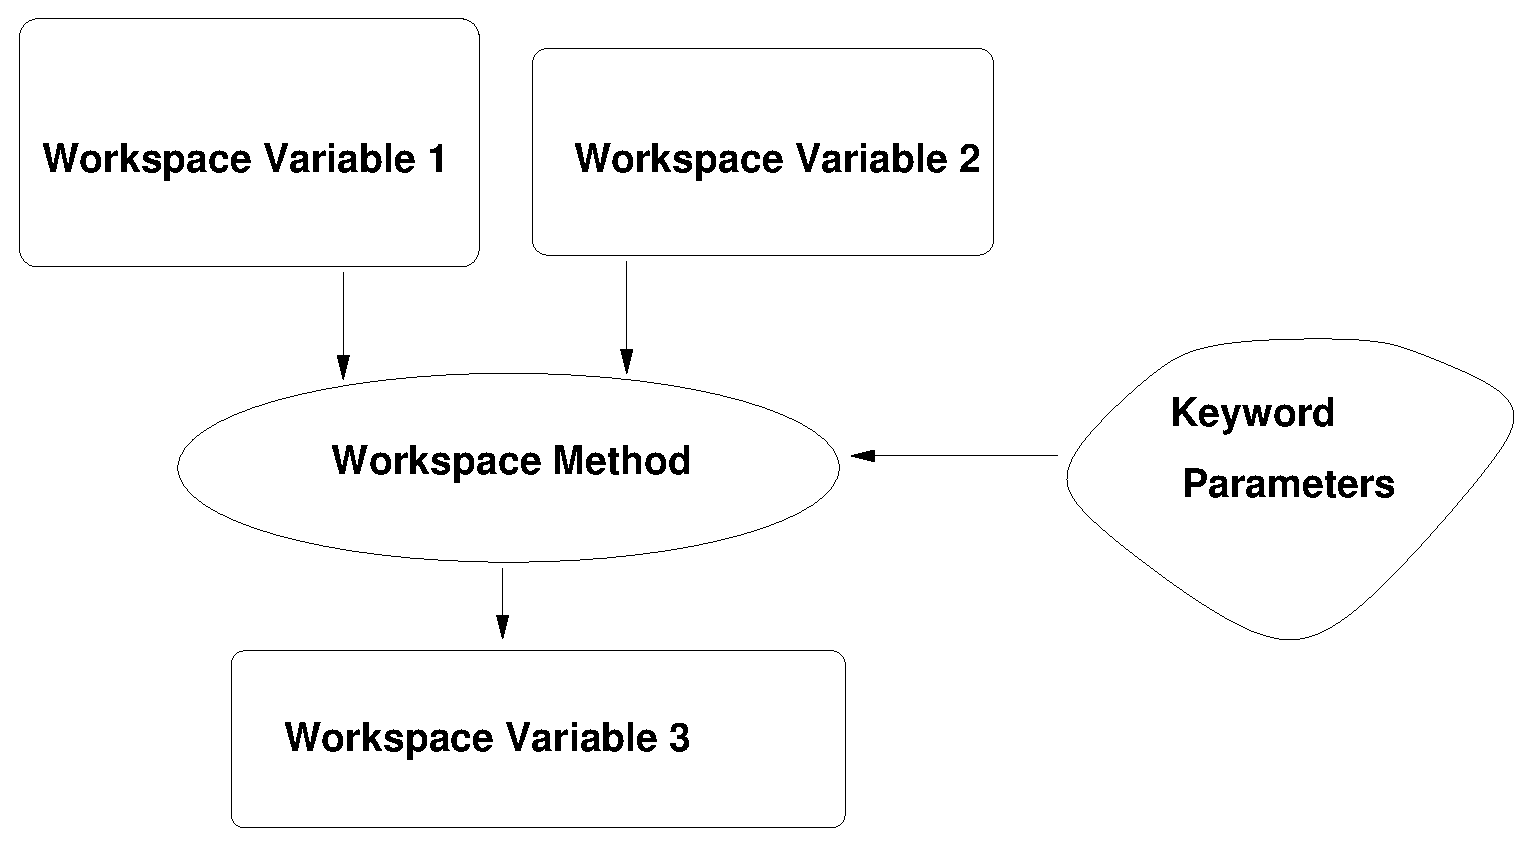
\includegraphics[width=\hsize,draft=false]{concept/method}
    \caption{\textindex{Specific
        workspace methods} act on specific workspace variables to
        generate other specific workspace variables. Additional input
        parameters can be specified as keyword parameters in the
        controlfile.}
    \label{fig:method}
  \end{center}
\end{figure}

It is important to note that the controlfile has a fixed and
well-defined syntax. This syntax is understood by the ARTS parser.
The great advantage of this concept is that it is very easy to add
new workspace variables and new workspace methods. The program has
an internal lookup table which lists all workspace methods, as well
as their input variables, output variables, and keyword
parameters. To add a new method, one just has to add an entry to
this lookup table, and write the code for the method itself. No
further changes to the program are necessary. In particular, no
changes to the program logic or to the parser. How such an extension
can be made practically is described in Section \ref{sec:development}.


\section{Generic Workspace Methods}
%=================================
\label{sec:concept:generic}

Generic methods (Figure \ref{fig:generic_method}) allow the user of
the program even more freedom than specific methods. A generic method
is for example \artsstyle{MatrixSet}, which can be used to set any
workspace variable which is a matrix. For example
\begin{quote}
  \artsstyle{MatrixSet(z\_surface){0.0}}
\end{quote}
will set all elements of \artsstyle{z\_surface} to 0.0 (as long as
\artsstyle{nrows} and \artsstyle{ncols} are set).

\begin{figure}
  \begin{center}
    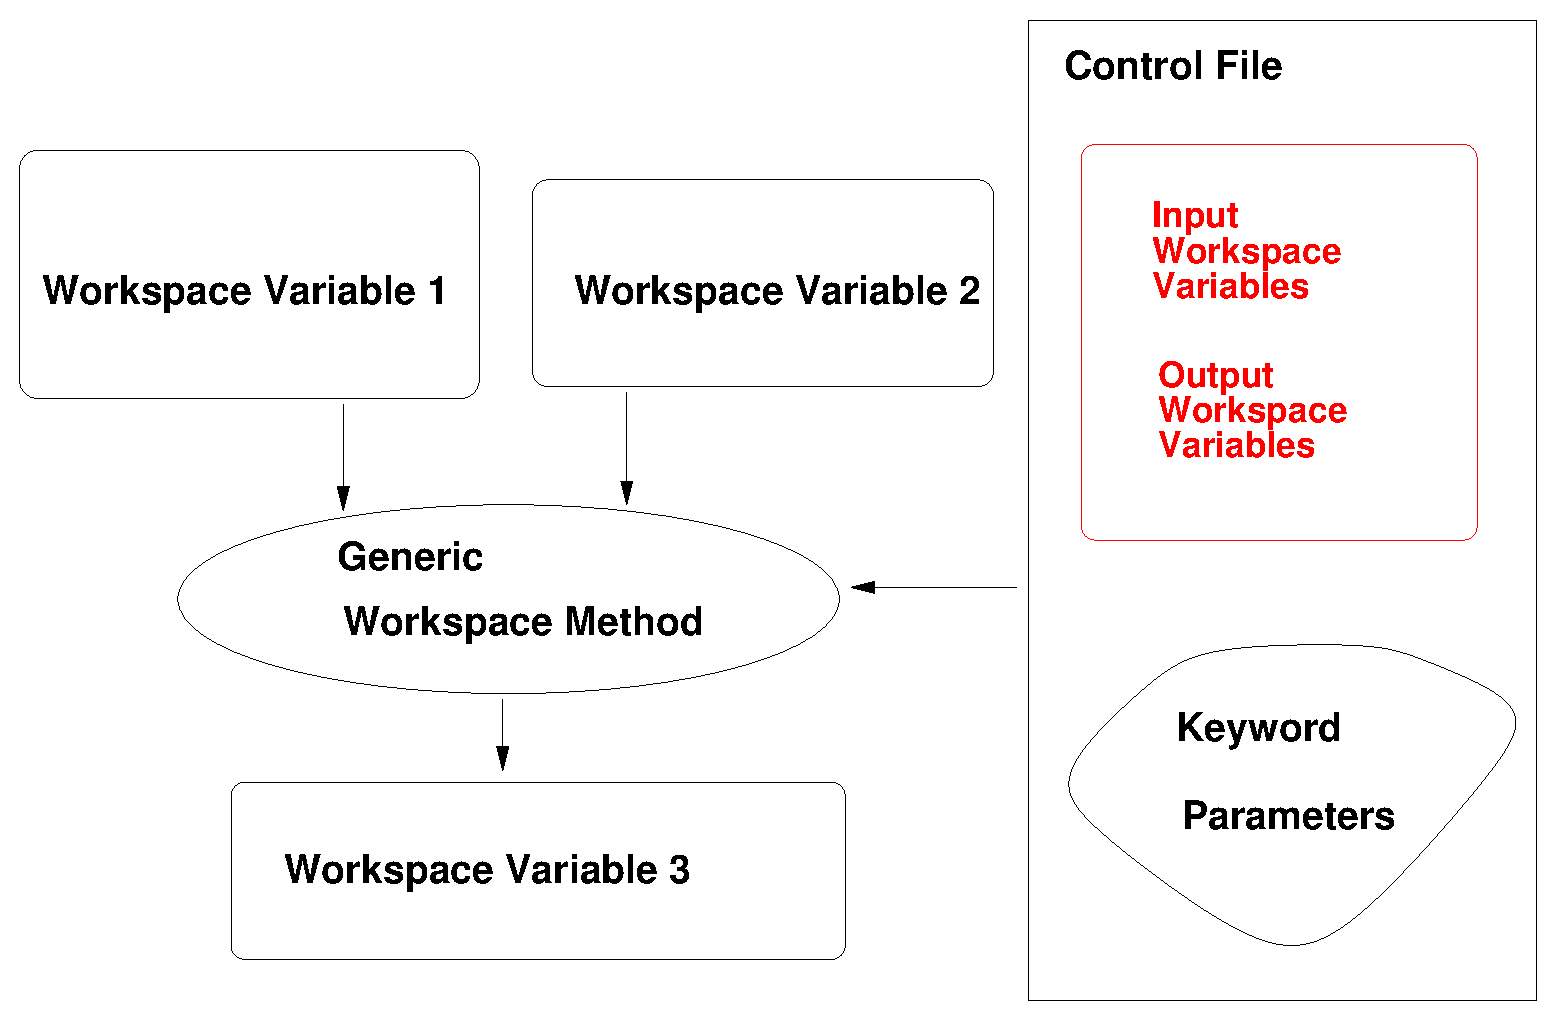
\includegraphics[width=\hsize,draft=false]{concept/generic_method}
    \caption{For \textindex{generic
      workspace methods} the workspace variables to act on are
        specified in the controlfile.}
    \label{fig:generic_method}
  \end{center}
\end{figure}

Some methods are even more flexible, the are super generic. This means
that they can take any workspace variable as input. The most commonly
used such methods are the XML file methods. A workspace variable is
read from a file in this way
\begin{quote}
  \artsstyle{ReadXML(f\_grid)\{"frequency\_grid"\}}
\end{quote}
Generic methods are particularly useful for IO operations like in the
example above. No new IO methods are necessary for new workspace
variables, as long as they are of standard types already known to the
program (for example vectors or matrices). 



\section{Agendas}
%=================================
\label{sec:concept:agendas}

Agendas are a special incarnation of a workspace method. In the
controlfile an arbitrary number of workspace methods can be added to
an agenda. On invocation, the agenda executes its methods one
after the other. The inputs and outputs defined for the agenda must
be satisfied by the invoked workspace methods. E.g., if an agenda
has \artsstyle{f\_grid} in its list of output workspace variables, a
workspace method which generates \artsstyle{f\_grid} must be added to
the agenda in the controlfile.

Even though it is possible to execute agendas directly from the
controlfile with the \artsstyle{AgendaExecute} method, the more common
and intended use case is the internal invocation by other workspace
methods. This adds a grave amount of flexibility to arts. The
\artsstyle{RteStd} method for example calculates (besides other
components) the emission term. Without the means of an agenda, it
would only be possible to use always the same method for the emission
calculation. By the use of an agenda the user can choose between
different methods to calculate the emission and plug them into the
emission agenda in the control file:

{\small
\begin{verbatim}
AgendaSet(emission_agenda){
  emissionPlanck{}
}
\end{verbatim}
}

\noindent
\artsstyle{RteStd} internally calls the \artsstyle{emission\_agenda} and
uses the user selected method for calculating the emission term.



\section{Practical hints}
%=================================
\label{sec:concept:practical}

The subdirectory \fileindex{tests} contains some example controlfiles.
You should study them to learn more about how the program works. You
can also run these controlfiles like this:
\begin{quote}
\begin{verbatim}
  arts simpleMC.arts
\end{verbatim}
\end{quote}
This assumes that you are inside the directory where the controlfiles
are, and that the \artsstyle{arts} executable is in your path.  You can
also run all of the examples, by saying
\begin{quote}
\begin{verbatim}
  make check
\end{verbatim}
\end{quote}

ARTS offers a number of useful command line parameters. In general,
there is a short form and a long form for each parameter. The short
form consists of a minus sign and a single letter, whereas the long
form consists of two minus signs and a descriptive name. To get a full
list, type
\begin{quote}
\begin{verbatim}
  arts -h
\end{verbatim}
\end{quote}
or
\begin{quote}
\begin{verbatim}
  arts --help
\end{verbatim}
\end{quote}
Most useful at the beginning should be the \artsstyle{-d}
(\artsstyle{--describe}), \artsstyle{-m} (\artsstyle{--methods}), \artsstyle{-w}
(\artsstyle{--workspacevariables}), and \artsstyle{-i} (\artsstyle{--input}) flags.
For instance, the \artsstyle{-d} (\artsstyle{--describe}) flag gives you online
documentation for any workspace method or workspace variable. Usage:
\begin{quote}
\begin{verbatim}
  arts -d f_grid
\end{verbatim}
\end{quote}
will print documentation about the workspace variable \artsstyle{f\_grid}, which
happens to be the monochromatic frequency grid.

But what methods and variables are available? You can find out by
typing
\begin{quote}
\begin{verbatim}
  arts -m all
\end{verbatim}
\end{quote}
which will list all workspace methods, or by typing 
\begin{quote}
\begin{verbatim}
  arts -w all
\end{verbatim}
\end{quote}
which will list all workspace variables. As you can see, these lists
are quite long. But you can get more specific information:
\begin{quote}
\begin{verbatim}
  arts -m f_grid
\end{verbatim}
\end{quote}
will give you a list of all methods that can generate the workspace
variable \artsstyle{f\_grid}. Specific and generic methods are listed
separately. Generic methods are in this case all methods producing a
Vector, since \artsstyle{f\_grid} belongs to this group. A similar task is
performed by the \artsstyle{-i} (\artsstyle{--input}) flag, with the difference
that \artsstyle{arts -i f\_grid} will list those methods that require
\artsstyle{f\_grid} as \emph{input}, whereas \artsstyle{arts -m f\_grid} lists
those that produce \artsstyle{f\_grid} as output. Finally,
\begin{quote}
\begin{verbatim}
  arts -w surfaceFlat
\end{verbatim}
\end{quote}
will give you all variables required by the method \artsstyle{abs\_coefCalc}
(the variable \artsstyle{f\_grid} happens to be one of them).

Using these command line parameters, it is easy to build up a
controlfile. The trick is, to start at the end. Say you want to
compute absorption coefficients. First of all, you have to find out
in which workspace variable these are stored. Look at the list
produced by \artsstyle{arts -w all}. You can use \artsstyle{arts -d} to look at
some candidates a bit more closely. This way, you will find out that
\artsstyle{abs\_coef} is the variable you are looking for.

In the next step, you can use \artsstyle{arts -m abs\_coef} to find all methods
that can calculate \artsstyle{abs\_coef}. So, you will find the method
\artsstyle{abs\_coefCalc}. Now you can use \artsstyle{arts -w abs\_coefCalc} to find out the
required input variables of that method. Then you can use the
\artsstyle{-m} flag again, to find the methods producing these variables,
and so on.

%%% Local Variables: 
%%% mode: latex
%%% TeX-master: "uguide"
%%% End: 

\chapter{Importing and exporting data}
 \label{sec:inout}


 \starthistory
 ? & ?.\\
 \stophistory

Sorry, so far just a few words about supported data formats.\\ \\

\FIXME{Extend this chapter.}


\section{Data formats}

\subsection{XML files}

% FIXME: OLE: Extend this
XML is the default file format for exchanging data with ARTS. Two flavors are
supported: Plain text and binary. In the plain format all data is stored in
the XML file. For binary, the structure of the data is stored in the XML file
and the data itself in binary format in a separate file.

\subsection{NetCDF files}

% FIXME: OLE: Extend this
NetCDF input and output is supported for a subset of the data types available
in ARTS.

\subsection{Gridded fields}

\subsubsection{Naming convention for grids}

% FIXME: OLE: Extend this
\begin{alltt}
\small
\input{gridded_field_gridnames.txt}
\end{alltt}



%%% Local Variables: 
%%% mode: latex
%%% TeX-master: "main"
%%% End: 

\chapter{Description of the atmosphere}
 \label{sec:atmosphere}

\starthistory
 130219 & Revised by Patrick Eriksson.\\ 
 020315 & First version by Patrick Eriksson.\\
\stophistory

\graphicspath{{Figs/atmosphere/}}

This section discusses the model atmosphere: how it is defined, its boundaries
and the variables describing the basic properties. One aspect that can cause
confusion is that several vertical coordinates must be used
(Sec.~\ref{sec:fm_defs:altitudes}). The main vertical coordinate is pressure
and atmospheric quantities are defined as a function of pressure
(Sec.~\ref{sec:fm_defs:grids}), but the effective vertical coordinate from a
geometrical perspective (such as the determination of propagation paths) is the
radius (Sec.~\ref{sec:fm_defs:atmdim}). Pressures and radii are linked by
specifying the geometrical altitudes (\builtindoc{z\_field}).


\section{Altitude coordinates}
%===================
\label{sec:fm_defs:altitudes}

\begin{description}
  
\item[Pressure\index{pressure}] The main altitude coordinate is
  pressure. This is most clearly manifested by the fact that the
  vertical atmospheric grid consists of equal-pressure levels.
  The vertical grid is accordingly denoted as the pressure grid and
  the corresponding workspace variable is \wsvindex{p\_grid}. The
  choice of having pressure as main altitude coordinate results in
  that atmospheric quantities are retrieved as a function of pressure.
  
\item[Pressure altitude\index{pressure altitude}] A basic assumption
  in ARTS is that atmospheric quantities (temperature, geometric
  altitude, species VMR etc.) vary linearly with the logarithm of the
  pressure. This corresponds roughly to assuming a linear variation
  with altitude. 

\item[Radius\index{radius}] Geometrical altitudes are
  needed to determine the propagation path through the atmosphere etc.
  The main geometrical altitude coordinate is the distance to the
  centre of the coordinate system used, the radius. This is a natural
  consequence of using a spherical or polar coordinate system. The
  radius is used inside ARTS for all geometrical calculations.
  
\item[Geometrical altitude\index{geometrical altitude}] The term geometrical
  altitude signifies here the difference in radius between a point and the
  reference ellipsoid (Sec.~\ref{sec:fm_defs:geoid}) along the vector to the
  centre of the coordinate system (Equation \ref{eq:fm_defs:zsurface}). This is
  consistent with the usage of geocentric latitudes (see below). Hence, the
  altitude is not measured along the local zenith direction.
\end{description}



\section{Atmospheric dimensionality}
%===================
\label{sec:fm_defs:atmdim}

The structure of the modelled atmosphere can be selected to have different
degree of complexity, the \textindex{atmospheric dimensionality}. There exist
three options, 1D, 2D and 3D, where 1D and 2D can be seen as special cases of
3D. The significance of these different atmospheric dimensionalities and the
geometrical coordinate systems used are described below in this section. The
atmospheric dimensionality is selected by setting the workspace variable
\wsvindex{atmosphere\_dim} to a value between 1 and 3. The atmospheric
dimensionality is most easily set by the functions \wsmindex{AtmosphereSet1D},
\wsmindex{AtmosphereSet2D} and \wsmindex{AtmosphereSet3D}.

\begin{figure}
 \begin{center}
  \includegraphics*[width=0.98\hsize]{atm_dim_1d}
  \caption{Schematic of a 1D atmosphere. The atmosphere is 
    here spherically symmetric. This means that the radius of the
    ellipsoid, the surface and all the pressure levels are constant
    around the globe. The fields are specified by a value for each
    pressure level. The extension of the cloud box is either from
    the surface up to a pressure level, or between two pressure
    levels (which is the case shown in the figure). The figure indicates
    also that the surface must be above the lowermost pressure
    level. (``Geoid'' in the legend should be ``Ellipsoid''.)}
  \label{fig:fm_defs:1d}  
 \end{center}
\end{figure}
% This figure was produced by the Matlab function mkfigs_atm_dims.

\begin{figure}
 \begin{center}
  \includegraphics*[width=0.98\hsize]{atm_dim_2d}
  \caption{Schematic of a 2D atmosphere. The radii (for the surface
    and the pressure levels) vary here linear between the latitude
    grid points. The atmospheric fields vary linearly along the
    pressure levels and the latitude grid points (that is, along the
    dotted lines). Inside the grid cells, the fields have a bi-linear
    variation. No cloud box is included in this figure.
    (``Geoid'' in the legend should be ``Ellipsoid''.)}
  \label{fig:fm_defs:2d}
 \end{center}
\end{figure}
% This figure was produced by the Matlab function mkfigs_atm_dims.

\begin{description}
  
\item[\textindex{1D}\,\,\,] A 1D atmosphere can be described as being
  spherically symmetric. The term 1D is used here for simplicity and historical
  reasons, not because it is a true 1D case (a strictly 1D atmosphere would
  just extend along a line). A spherical symmetry means that atmospheric fields
  and the surface extend in all three dimensions, but they have no latitude and
  longitude variation. This means that, for example, atmospheric fields vary
  only as a function of altitude and the surface constitutes the surface of a
  sphere. The radial coordinate is accordingly sufficient when dealing with
  atmospheric quantities. The latitude and longitude of the sensor are normally
  of no concern, but when required the sensor is considered to be placed at
  latitude and longitude zero $([\Lat,\Lon]=[0,0])$. The sensor is assumed to
  by directed towards the North pole, corresponding to an azimuth angle of
  0\degree. A 1D atmosphere is shown in Figure~\ref{fig:fm_defs:1d}.
  
\item[\textindex{2D}\,\,\,] In contrast to the 1D and 3D cases, a 2D atmosphere
  is only strictly defined inside a plane. More in detail, this case be seen as
  observations restricted to the plane where the longitude equals 0\degree\ or
  180\degree. A polar system\index{polar coordinate system}, consisting of a
  radial and an angular coordinate, is applied. The angular coordinate is
  denoted as latitude, and matches the 3D latitude in the range
  $[-90\degree,+90\degree]$, but for 2D there is no lower or upper limit for
  the latitude coordinate. The 2D case is most likely used for satellite
  measurements where the atmosphere is observed inside the orbit plane. The 2D
  ``latitude'' can then be taken as the angular distance along the satellite
  track. A 2D-latitude of e.g.\ 100\degree\ will then correspond to a
  3D-latitude of 80\degree. The atmosphere is normally treated to be undefined
  outside the considered plane, but some scattering calculations may treat the
  surrounding atmosphere in an simplified manner. A 2D atmosphere is shown in
  Figure~\ref{fig:fm_defs:2d}.

\item[\textindex{3D}\,\,\,] In this, the most general, case, the atmospheric
  fields vary in all three spatial coordinates, as in a true atmosphere
  (Figures~\ref{fig:fm_defs:3d}). A
  \textindex{spherical coordinate system} is used where the dimensions are
  radius (\Rds), latitude (\Lat) and longitude (\Lon), and a position is given
  as $(\Rds,\Lat,\Lon)$. With other words, the standard way to specify a
  geographical position is followed. The valid range for latitudes is
  $[-90\degree,+90\degree]$, where +90\degree corresponds to the North pole
  etc. Longitudes are counted from the Greenwich meridian with positive values
  towards the east. Longitudes can have values from -360\degree to +360\degree.
  When the difference between the last and first value of the longitude grid is
  $360\degree$ then the whole globe is considered to be covered. The user
  must ensure that the atmospheric fields for \Lon\ and $\Lon+360\degree$ are
  equal. If a point of propagation path is found to be outside the range of the
  longitude grid, this will results in an error if not the whole globe is
  covered. When possible, the longitude is shifted with 360\degree\ in the
  relevant direction.
  

\end{description}

\begin{figure}[t]
 \begin{center}
  \includegraphics*[angle=-90,width=0.98\hsize]{atm_dim_3d}
  \vspace*{-15mm}
  \caption{Schematic of a 3D atmosphere. Plotting symbols as in 
    Figure \ref{fig:fm_defs:2d}. Radii and fields are here defined to
    vary linearly along the latitude and longitude grid points. This
    means that the radius of a pressure level has a
    bi-linear variation inside the area limited by two latitude and
    longitude grid values, while the atmospheric fields have a
    tri-linear variation inside the grid cells. }
  \label{fig:fm_defs:3d}
 \end{center}
\end{figure}
% This figure was produced by the Matlab function mkfigs_atm_dims.



\section{Atmospheric grids and fields}
%===================
\label{sec:fm_defs:grids}

As mentioned above, the vertical grid of the atmosphere consists of a
set of layers with equal pressure, the pressure grid
(\wsvindex{p\_grid}).  This grid must of course always be specified.
The upper end of the pressure grid gives the practical upper limit of
the atmosphere as vacuum is assumed above. With other words, no
absorption and refraction take place above the uppermost pressure
level.

A \textindex{latitude} grid (\wsvindex{lat\_grid}) must be specified for 2D and
3D. For 2D, the latitudes shall be treated as the angular distance along the
orbit track, as described above in Section~\ref{sec:fm_defs:atmdim}. The
latitude angle is throughout calculated for the vector going from the centre of
the coordinate system to the point of concern. Hence, the latitudes here
correspond to the definition of the geocentric latitude, and not geodetic
latitudes (Sec.~\ref{sec:ppath:geoid}). This is in accordance to the
definition of geometric altitudes (Sec.~\ref{sec:fm_defs:altitudes}). For
3D, a \textindex{longitude} grid (\wsvindex{lon\_grid}) must also be specified.
Valid ranges for latitude and longitude values are given in
Section~\ref{sec:fm_defs:atmdim}. If the longitude and latitude grids are not
used for the selected atmospheric dimensionality, then the longitude grid (for
1D and 2D) and the latitude grid (for 1D) must be set to be empty.

The atmosphere is treated to be undefined outside the latitude and longitude
ranges covered by the grids, if not the whole globe is covered. This results in
that a propagation path is not allowed to cross a latitude or longitude end
face of the atmosphere, if such exists, it can only enter or leave the
atmosphere through the top of the atmosphere (the uppermost pressure level).
See further Section~\ref{sec:fm_defs:ppaths}. The volume covered by the grids
is denoted as the \textindex{model atmosphere}.

The basic atmospheric quantities are represented by their values at each
crossing of the involved grids (indicated by thick dots in Figure
\ref{fig:fm_defs:2d}), or for 1D at each pressure level (thick dots in Figure
\ref{fig:fm_defs:1d}). This representation is denoted as the
field\index{atmospheric field} of the quantity. The field must, at least, be
specified for the geometric altitude of the pressure levels
(\wsvindex{z\_field}), the temperature (\wsvindex{t\_field}) and considered
atmospheric species (\wsvindex{vmr\_field}). The content and units of
\builtindoc{vmr\_field} are discussed in
Section~\ref{sec:rteq:absspecies}.

All the fields are assumed to be piece-wise linear functions vertically (with
pressure altitude as the vertical coordinate), and along the latitude and
longitude edges of 2D and 3D grid boxes. For points inside 2D and 3D grid
boxes, multidimensional linear interpolation is applied (that is, bi-linear
interpolation for 2D etc.). Note especially that this is also valid for the
field of geometrical altitudes (\builtindoc{z\_field}). Fields are rank-3
tensors. For example, the temperature field is $T=T(\Prs,\Lat,\Lon)$. That
means each field is like a book, with one page for each pressure grid point,
one row for each latitude grid point, and one column for each longitude grid
point. In the 1D case there is just one row and one column on each page. The
representation of atmospheric fields, and other quantities, is discussed
further in Section~\ref{sec:wfuns:basis}, where the concept of basis
functions\index{basis function} is introduced. In short, the basis functions
give the mapping from the set of discrete values to the continuous
representation of the quantity.



\section{Geo-location of 1D and 2D}
%===================
\label{sec:fm_defs:geoloc}

For 1D and 2D atmospheres, \builtindoc{lat\_grid} and \builtindoc{lon\_grid} do
not contain true geographical positions (they are either empty or
\builtindoc{lat\_grid} contains transformed data). However, some operations
require that the positions is known, and this \index{geo-location} is handled
by \wsvindex{lat\_true} and \wsvindex{lon\_true}. See the built-in
documentation for further information on how to specify these variables.



\section{Hydrostatic equilibrium}
%===================
\label{sec:fm_defs:hse}

There is no general demand that the model atmosphere fulfils hydrostatic
equilibrium. That is, \builtindoc{t\_field} and \builtindoc{z\_field} can be
specified independently of each other. On the other hand, ARTS provides means
for ensuring that a model atmosphere matches hydrostatic equilibrium by the
method \wsmindex{z\_fieldFromHSE}. The method considers that gravitation varies
with latitude and altitude, and \builtindoc{lat\_true} and
\builtindoc{lon\_true} must be set for 1D and 2D.

Hydrostatic equilibrium gives only constrain for the distance between the
pressure levels, not for the absolute geometrical altitudes. For this reason, a
``reference point'' must be introduced. This is done by setting the pressure of
this point by \wsvindex{p\_hse} (common for all latitude and longitudes). The
geometrical altitudes matching \builtindoc{p\_hse} are taken from the original
values in \wsvindex{z\_field}. 


\section{The reference ellipsoid and the surface}
%===================
\label{sec:fm_defs:surf}

Geometrical altitudes are specified as the vertical distance to the reference
ellipsoid (\wsvindex{refellipsoid}), discussed further in
Section~\ref{sec:fm_defs:geoid}. The lower boundary of the atmosphere is
denoted as the surface. The surface is specified by its geometrical altitude on
the latitude and longitude grids. The workspace variable holding these data is
called \wsvindex{z\_surface}.

It is not allowed that there is an altitude gap between the surface and
the lowermost pressure level.  That is, the surface pressure must be
smaller than the pressure of the lowermost vertical grid level. On
the other hand, it is not necessary to match the surface and the first
pressure level, the pressure grid can extend below the surface level.


\section{The cloud box}
%===================
\label{sec:fm_defs:cloudbox}
In order to save computational time, calculations involving scattering are
limited to a special atmospheric domain. This atmospheric region is denoted as
the \textindex{cloud box}. The distribution of scattering matter inside the
cloud box is specified by \wsvindex{pnd\_field}, see further
Section~\ref{sec:rteq:absspecies}.

The cloud box is defined to be rectangular in the used coordinate
system, with limits exactly at points of the involved grids. This
means, for example, that the vertical limits of the cloud box are two
pressure levels. For 3D, the horizontal extension of the cloud box
is between two points of the latitude grid and likewise in the
longitude direction (Fig.~\ref{fig:fm_defs:3dcross}). The latitude
and longitude limits for the cloud box cannot be placed at the end
points of the corresponding grid as it must be possible to calculate
the incoming intensity field. The cloud box is activated by setting
the variable \wsvindex{cloudbox\_on} to 1.  The limits of the cloud
box are stored in \wsvindex{cloudbox\_limits}.  It is recommended to
use the method \wsmindex{cloudboxOff} when no scattering calculations
shall be performed. This method assigns dummy values to all workspace
variables not needed when scattering is neglected.

\FIXME{add info on available cloudbox setting methods. particularly manual and
automatic methods and which fields the latter look at}

\begin{figure}[!t]
 \begin{center}
  \includegraphics*[width=0.98\hsize]{atm_dim_3dcross}
  \caption{A latitudinal, or longitudinal, cross section of a 3D atmosphere. 
    Plotting symbols as in Figure \ref{fig:fm_defs:1d}. Radii and
    fields inside the cross section match the definitions for 2D.
    The vertical extension
    of the cloud box is defined identical for 1D and 3D. The horizontal 
    extension of the cloud box is between two latitude and longitude grid
    positions, where only one of the dimensions is visible in this figure.}
  \label{fig:fm_defs:3dcross}
 \end{center}
\end{figure}
% This figure was produced by the Matlab function mkfigs_atm_dims.

When the radiation entering the cloud box is calculated this is done
with the cloud box turned off. This to avoid to end up in the
situation that the radiation entering the cloud box depends on the
radiation coming out from the cloud box. {\bf It is the task of the
  user to define the cloud box in such way that the link between the
  outgoing and ingoing radiation fields of the cloud box can be
  neglected}. The main point to consider here is radiation reflected
by the surface. To be formally correct there should never be a gap
between the surface and the cloud box. This is the case as radiation
leaving the cloud box can then be reflected back into the cloud box by
the surface. If it is considered that the surface is a scattering object
it is clear that the surface should in general be part of the cloud
box. However, for many cases it can be accepted to have a gap between
the surface and the cloud box, with the gain that the cloud box can be
made smaller. Such a case is when the surface is treated to act as
blackbody, the surface is then not reflecting any radiation.
Reflections from the surface can also be neglected if the zenith
optical thickness of the atmosphere between the surface and cloud box
is sufficiently high.


\section{Wind vector fields}
\label{sec:atm:windfields}
%
The atmospheric fields discussed above are scalar quantities, while some
atmospheric variables can be seen as vector fields. However, in ARTS input
vector fields are broken down into the zonal, meridional and vertical
components and are given as three scalar fields. This division into scalar
values is used to allow that one or several of the components easily can be set
to zero, which is done by setting the corresponding workspace variable to be
empty. Following the standard naming scheme for winds, the components are
denoted as
\begin{description}
\item[u] The zonal component. A positive value signifies an Eastward direction.
\item[v] The meridional component. A positive value signifies a Northward
  direction.
\item[w] The vertical component. A positive value signifies an upward
  direction.
\end{description}
The workspace variables to describe the wind vector field are
\wsvindex{wind\_u\_field}, \wsvindex{wind\_v\_field} and
\wsvindex{wind\_w\_field}. To clarify the definition of the vector components
above, the winds components are defined as follows
\begin{itemize}
\item[\WindWE] A positive wind is defined as air moving
  from west to east, i.e.\ towards higher longitudes.
\item[\WindSN] A positive wind is defined as air
  moving from south to north, i.e.\ towards higher latitudes.
\item[\WindVe] A positive wind is defined as air
  moving upwards, i.e.\ towards higher altitudes.
\end{itemize}
As described above, one, two or all of these variables can be set to be empty,
if the corresponding wind component is zero.

Winds affect the radiative transfer by inducing Doppler shifts, see further
Chapter~\ref{sec:winds}. Note that \WindWE\ causes no Doppler shift for 1D and 2D
atmospheric setups. Considering the sensor viewing conventions in the 1D
atmosphere case as laid out in Sec.~\ref{sec:fm_defs:atmdim}, positive \WindSN\
correspond to tail winds, negative to head winds.


\section{Magnetic field vector fields}
\label{sec:atm:magfields}

To consider Faraday rotation (Sec.~\ref{sec:faraday}) and Zeeman splitting
(Sec.~\ref{sec:absorption:zeeman}), the \textindex{magnetic field} must
be specified. The same strategy of specifying the vector field by three scalar
components is applied as for the winds field (see above).

The three component fields are \wsvindex{mag\_u\_field},
\wsvindex{mag\_v\_field} and \wsvindex{mag\_w\_field}. All three components
must be specified (but can be set to zero for a part of, or the complete,
atmosphere). However, some component can be irrelevant for the calculations.
For example, the u-component has no influence on Faraday rotation for 1D and 2D
cases. (The internal representation of the magnetic field at a specific point
is handled by \wsvindex{rtp\_mag}. For this variable the three components are
stored together, and thus the local magnetic field is represented as a vector.)




%%% Local Variables: 
%%% mode: latex
%%% TeX-master: "uguide"
%%% End: 

\chapter{Radiative transfer basics}
 \label{sec:rte_basics}


 \starthistory
 130212 & Started (Patrick Eriksson).\\
 \stophistory

 This chapter introduces some basic radiative transfer nomenclature and
 equations. The radiative transfer equation is here presented in quite general
 terms, while special cases and solutions are discussed in later parts of the
 document. 


\section{Stokes dimensionality}
%==============================================================================
\label{sec:fm_defs:polarisation}

The full polarisation state of radiation can be described by the Stokes vector,
and is the formalism applied in ARTS. The vector can be defined in different
ways, but it has always four elements. The Stokes vector, \StoVec, is here
written as
\begin{equation}
  \label{eq:fm_defs:stokevec}
  \StoVec = \left[
  \begin{array}{c}
   \StoI\\ \StoQ \\ \StoU\\ \StoV
  \end{array}
  \right],
\end{equation}
where the first component (\StoI) is the full intensity of the
radiation, the second component (\StoQ) is the difference between
vertical and horizontal polarisation, the third component (\StoU) is the
difference for $\pm$45$^\circ$ polarisation and the last component
(\StoV) is the difference between left and right circular polarisation.
That is:
\begin{eqnarray}
  \StoI &=&   \Iv + \Ih = \Ipff + \Imff = \Ilhc + \Irhc, \\
  \StoQ &=&   \Iv - \Ih,                                 \\
  \StoU &=&   \Ipff - \Imff,                             \\
  \StoV &=&   \Ilhc - \Irhc,                             
\end{eqnarray}
where \Iv, \Ih, \Ipff, and \Imff\ are the intensity of the component linearly
polarised at the vertical, horizontal, +45\degree\ and -45\degree\ direction,
respectively, and \Irhc, and \Ilhc\ are the intensity for the right- and
left-hand circular components. Further details on polarisation and the
definition of the Stokes vector are found in \theory,
Section~\ref{T-sec:polarization}.

ARTS is a fully polarised forward model, but can be run with a smaller
number of Stokes components. The selection is made with the workspace
variable \wsvindex{stokes\_dim}. For example, gaseous absorption and
emission are in general unpolarised, and if not scattering has to be
considered it is sufficient to only include the first Stokes
components in the simulations. To include higher order Stokes
components results only, in this case, in slower calculations. The
general case is here denoted as \textindex{vector radiative transfer},
while \textindex{scalar radiative transfer} refers to the case when
only the first Stokes component is considered.
 


\section{The radiative transfer equation}
%==============================================================================
\label{sec:rteq}

The radiative transfer problem can only be expressed in general terms as a
differential equation. One version for vector radiative transfer is
\begin{equation}
    \label{eq:VRTE0}
  \frac {\DiffD\StoVec(\Frq,\PPos,\PDir)}{\DiffD s} =
    -\ExtMat(\Frq,\PPos,\PDir) \StoVec(\Frq,\PPos,\PDir) +
    \VctStl{j}_e(\Frq,\PPos,\PDir) + \VctStl{j}_s(\Frq,\PPos,\PDir),  
\end{equation}
where \Frq\ is frequency, \PPos\ represents the atmospheric position, \PDir\ is
the propagation direction (at \PPos), $s$ is distance along \PDir, $\ExtMat$ is
the extinction matrix, $\VctStl{j}_e$ is the emission at the point
and $\VctStl{j}_s$ represents the scattering from other directions into the
propagation direction.


\subsection{Main cases}
\label{sec:rteq:cases}
%
One of the general assumptions in ARTS is that local thermodynamic equilibrium
(LTE) can be assumed. If we for the moment assume that scattering can be
totally neglected then Equation~\ref{eq:VRTE0} becomes
\begin{equation}
  \label{eq:VRTE1}
  \frac{\DiffD\StoVec(\Frq,\PPos,\PDir)}{\DiffD s} =
    \ExtMat_a(\Frq,\PPos,\PDir)\left[ \VctStl{s}- \StoVec(\Frq,\PPos,\PDir)
    \right],
\end{equation}
where $\ExtMat_a$ is denoted as the absorption matrix (to flag that it contains
no contribution from scattering) and \VctStl{s} can be seen as the emission
source vector, defined as
\begin{equation}
  \VctStl{s} = [B(\Frq,\PPos),0,0,0]^T,
\end{equation}
where $B$ is the Planck function, describing blackbody radiation. Cases, where
Equation~\ref{eq:VRTE1} is valid, are in ARTS denoted as ``clear-sky''
radiative transfer (implying LTE if nothing else is stated). The discussion of
such radiative transfer calculations is continued in Section~\ref{sec:rte}. The
atmospheric quantities contributing to $\ExtMat_a$ already for clear-sky
conditions are denoted as ``absorbing species''.

Some additional conditions are required to put scattering into the picture. If
scattering is of incoherent and elastic nature, the extension of 
Equation~\ref{eq:VRTE1} is
\begin{eqnarray}
  \label{eq:VRTE2}
  \frac {\DiffD\StoVec(\Frq,\PPos,\PDir)}{\DiffD s} &=&
    -\ExtMat(\Frq,\PPos,\PDir) \StoVec(\Frq,\PPos,\PDir) +
    \ExtMat_a(\Frq,\PPos,\PDir)\VctStl{s} + \\ \nonumber
    &&+ \int_{4\pi} \DiffD\PDir' \PhaMat(\Frq,\PPos,\PDir,\PDir')
    \StoVec(\Frq,\PPos,\PDir'),
\end{eqnarray}
where $\PhaMat$ is the scattering (or phase) matrix (and
$\ExtMat\neq\ExtMat_a$). The aerosol, cloud or precipitation objects that
cause \PhaMat\ to deviate from zero (and contribute to \ExtMat\ and $\ExtMat_a$)
are simply denoted as ``particles'', and the solution of
Equation~\ref{eq:VRTE2} is referred to as ``scattering calculations''. ARTS
includes several modules to handle scattering, introduced in the last part of
this document.

Equation~\ref{eq:VRTE2} is discussed quite thoroughly in \ref{T-sec:rte_theory}
of \theory. This including that for some conditions also the ``n2-law of
radiance'' must be considered to obtain completely exact results. For further
discussion of this issue, see first of all Section~\ref{sec:fm_defs:unit}.



\subsection{Some comments and nomenclature}
\label{sec:rteq:names}
%
The equations above treat a single frequency and a single direction, at a
time, and can be said to describe monochromatic pencil beam radiative
transfer. For simplicity, the frequency and direction are left out from many of
the equations in this user guide. 
Some further information around the involved radiative quantities:
\begin{description}
\item[\StoVec] As workspace variable denoted as \wsvindex{iy}. The variable can
  hold \StoVec\ for a range of frequencies, but covers only radiative transfer
  along a single propagation path. Please note the distinction to \wsvindex{y},
  that holds radiances from several frequencies and pencil beams, possibly
  weighted with some instrument responses.
%\item[\ExtMat] In the most general case, this matrix can cover three
%  different physical mechanisms: absorption, scattering and magneto-optical
%  effects. The sum of absorption and scattering is denoted as extinction.
%  An example on magneto-optical effect is Faraday rotation, that is not
%  changing the radiation intensity, but the polarisation state.
%
%  Inside ARTS, \ExtMat\ treated as a sum of two parts:
%  $\ExtMat=\ExtMat_a\ExtMat_p$, where the first part, $\ExtMat_a$, corresponds
%  to the ``absorbing species'', while the second part, $\ExtMat_a$, covers the
%  extinction of the (scattering) ``particles''. As workspace variables,
%  $\ExtMat_a$ and $\ExtMat_p$ are called \wsvindex{propmat\_clearsky} and
%  \wsvindex{propmat\_particle}, respectively.

\item[B] The corresponding workspace variable is
  \wsvindex{blackbody\_radiation}.

%\item[$\VctStl{j}_e$] is denoted as the \wsvindex{emission\_vector}. 



\end{description}

\chapter{Complete calculations}
 \label{sec:complcalcs}

\starthistory
 130219 & First version by Patrick Eriksson.\\
\stophistory

\graphicspath{{Figs/rte/}}

This chapter outlines how complete radiative transfer simulations are
performed. ARTS is not only performing atmospheric radiative transfer, also
sensor characteristics can be considered. As a consequence, the topics of this
chapter include the distinction between monochromatic pencil beam and ``full''
calculations, and how the sensor is introduced.



\section{Overview}
%
An attempt to illustrate a ``standard'' ARTS calculation is found in Figure~
\ref{fig:ycalc_flow}. The figure shows that most calculation tasks are handled
by an agenda. For example, \builtindoc{ppath\_agenda} has the task of
determining the propagation path for the given observation geometry. In
principle, the agenda could solve the task by loading data from a file, but
most likely it will use some of the dedicated workspace methods. These
workspace methods are targeted towards different observation types, for
example, radio link calculations require special consideration. Anyhow, the
main message here is that by using the agenda concept, a very high degree of
flexibility can be achieved and new features can be added fairly simply. On the
other hand, the concept require that the user actually apply methods that make
sense for the agenda. The code of ARTS performs some consistency checks of the
agenda output, but this can only catch some types of mistakes.

Complete radiative transfer calculations are normally performed by
\wsmindex{yCalc}. This method incorporates sensor responses and has the
variable \wsvindex{y} as main output. The letter y here refers to the
measurement vector, \MsrVct, found in the formalism of
\citet{rodgers:90,rodgers:00} (see also Sec.~\ref{T-sec:formalism:wfuns} of
\theory). The vector can hold anything from a single value, to a high number of
spectra appended. The spectra in the last case can correspond to a limb
sounding sequence (hence measured for different zenith angles), or even be
measured by different sensors. In any case, the data in \MsrVct\ contain likely
significant impact of different parts of the sensor used, such as the angular
weighting by the antenna pattern. 

\begin{figure*}[p]
 \begin{center}
  \includegraphics*[clip,trim=25 30 25 40,width=0.99\hsize]{ycalc_flow}\\
  {\small (For caption see top of the next page.)}
 \end{center}
\end{figure*}
% This figure was produced by LibreOffice draw: ycalc_flow.odg

\begin{figure}[t]
  \caption{A flowchart of a radiative transfer calculation (on previous page),
    using \wsmindex{yCalc} or \wsmindex{iyCalc}. The figure assumes that
    \wsaindex{iy\_main\_agenda} holds \wsmindex{iyEmissionStandard}, that
    represents the most complex case. Some important input data are shown in
    orange, and main output are shown in green. The two main methods are
    plotted as grey boxes, while agendas are shown as ovals. For
    connections between methods and agendas the arrows show the direction of
    output (calculated) data. Every call of an agenda involves also some input
    data (settings), but this aspect has been ignored for clarity reasons. Data
    entering an agenda along a common line indicates mutually independent
    options. For example, absorption can be calculated "on-the-fly" from basic
    spectroscopic data or be extracted from a pre-calculated look-up table (see
    bottom-right corner). The dotted lines indicate that some methods and
    agendas can make further calls of \builtindoc{iy\_main\_agenda}.}
  \label{fig:ycalc_flow}
\end{figure}

On the other hand, atmospheric radiative transfer is performed for
monochromatic frequencies, along pencil beam directions. The outcome of one
such calculation is the Stokes vector for each frequency considered, and as
workspace variable this quantity is denoted as \wsvindex{iy}. Please, note the
distinction to \builtindoc{y}, that can contain information from a number of
monochromatic pencil beam calculations, as shown in
Section~\ref{sec:fm_defs:seqsandblocks}.

Further, the term ``iy'' is not restricted to the final outcome of atmospheric
radiative transfer, it is also used to indicate that quantities and operations
are of monochromatic pencil beam character. For example, the agenda returning
the radiation entering the atmosphere from space is named as
\builtindoc{iy\_space\_agenda} to indicate that the agenda output is directly
associated with the calculation of \builtindoc{iy}. If only a single
\builtindoc{iy} is of concern, the radiative transfer can be performed by
\wsmindex{iyCalc}, having a smaller set of input arguments than
\builtindoc{yCalc}.

The output is not restricted to \builtindoc{y} or \builtindoc{iy}, also some
auxiliary data can be extracted as described in Section~\ref{sec:fm_defs:aux}.
In addition, \builtindoc{yCalc} can also provide weighting functions
(Chapter~\ref{sec:wfuns}).








\section{Compulsory sensor and data reduction variables}
%==============================================================================
\label{sec:fm_defs:sensor1}

The instrument real or hypothetical, that detects the simulated radiation is
denoted as the sensor\index{sensor, the}. The forward model is constructed in
such way that a sensor must exist. For cases when only monochromatic pencil
beam radiation is of interest, the positions and directions for which the
radiation shall be calculated are given by specifying an imaginary sensor with
infinite frequency and angular resolution. The workspace variables for the
sensor that always must be specified are \builtindoc{sensor\_response},
\builtindoc{sensor\_pos}, \builtindoc{sensor\_los} and
\builtindoc{mblock\_dlos\_grid}. These variables are presented separately
below.


\subsection{Sensor position\index{sensor position}}
%===================
\label{sec:fm_defs:sensorpos}

The observation positions of the sensor are stored in
\wsvindex{sensor\_pos}. This is a matrix where each row corresponds to
a sensor position. The number of columns in the matrix equals the
atmospheric dimensionality (1 column for 1D etc.). The columns of the
matrix (from first to last) are geometrical altitude, latitude and longitude.
Accordingly, row $i$ of \builtindoc{sensor\_pos} for a 3D case is
$(\aAlt{i},\aLat{i},\aLon{i})$. The sensor position can be set to any
value, but the resulting propagation paths (also dependent on
\builtindoc{sensor\_los}) must be valid with respect to the model
atmosphere (see Section~\ref{sec:fm_defs:ppaths}). An obviously
incorrect choice is to place the senor below the surface altitude. If
the sensor is placed inside the model atmosphere, any sensor
line-of-sight is allowed, this including the cases that the sensor is
placed on the surface looking down, and that the sensor is placed
inside the cloud box. 

One or several spectra can be calculated for each position as described in
Section~\ref{sec:fm_defs:seqsandblocks}. The corresponding workspace variable
for single pencil beam calculations is \wsvindex{rte\_pos}, that is an input
argument to e.g.\ \wsaindex{iy\_main\_agenda} and \wsmindex{iyCalc}.



\subsection{Line-of-sight\index{line-of-sight}}
%===================
\label{sec:fm_defs:los}

The viewing direction of the sensor, the line-of-sight, is described
by two angles, the zenith angle (\ZntAng) and the azimuth angle
(\AzmAng). The zenith angle exists for all atmospheric
dimensionalities, while the azimuth angle is defined only for 3D.
The term line-of-sight is not only used in connection with the sensor,
it is also used to describe the local propagation direction along the
path taken by the observed radiation
(Section~\ref{sec:fm_defs:ppaths}).  The zenith and azimuth angles
are defined in an identical way in both of these contexts (sensor
pointing direction; local propagation direction). This is expected as
the position of the sensor is the end point of the propagation path.
The sensor line-of-sight is the direction the antenna is pointed to
receive the radiation. The line-of-sight for propagation paths is
defined likewise, it is the direction in which a hypothetical sensor
must be placed to receive the radiation along the propagation path at
the point of interest. This means that the line-of-sight and the
photons are going in opposite directions. As a true sensor has a
finite spatial resolution (described by the antenna pattern),
theoretically there is an infinite number of line-of-sights associated
with the sensor, but in the forward model, spectra are only calculated
for a discrete set of directions. If a sensor line-of-sight is
mentioned without any comments, it refers to the direction in which
the centre of the antenna pattern is directed.

\begin{figure}
 \begin{center}
  \begin{minipage}[c]{0.6\textwidth}
   \includegraphics*[width=0.99\hsize]{za_and_aa_angles}
  \end{minipage}%
  \begin{minipage}[c]{0.4\textwidth}
   \caption{Definition of zenith angle, \ZntAng, and azimuth angle, 
       \AzmAng, for a line-of-sight. The figure shows a line-of-sight
       with a negative azimuth angle.}
   \label{fig:fm_defs:los}
  \end{minipage}
 \end{center}
\end{figure}           
 
The \textindex{zenith angle}, \ZntAng, is simply the angle between the
line-of-sight and the zenith direction (Figure~\ref{fig:fm_defs:los}).
The valid range for 1D and 3D cases is $[0,180\degree]$. In the case
of 2D, zenith angles down to -180\degree\ are also allowed, where the
distinction is that positive angles mean a viewing direction towards
higher latitudes, and negative angles mean a viewing direction towards
lower latitudes. It should be mentioned that the zenith and nadir
directions are here defined to be along the line passing the centre of
the coordinate system and the point of concern
(Section~\ref{sec:ppath:geoid}). A nadir observation,
$\ZntAng=180\degree$, is thus a measurement towards the centre of the
coordinate system.

The \textindex{azimuth angle}, \AzmAng, is given with respect to the
\textindex{meridian plane}.  That is, the plane going through the
north and south poles of the coordinate system $(\Lat=\pm90\degree)$
and the sensor. The valid range is $[-180\degree,180\degree]$ where
angles are counted clockwise; 0\degree means that the viewing or
propagation direction is north-wise and +90\degree\ means that the
direction of concern goes eastward. This definition does not work for
position on the poles. To cover these special cases, the definition is
extended to say that for positions on the poles the azimuth angle
equals the longitude along the viewing direction. For example, if
standing on any of the poles and the viewing direction is towards
Greenwich, the azimuth angle is 0\degree.

The sensor line-of-sights are stored in \wsvindex{sensor\_los}. This workspace
variable is a matrix, where the first column holds zenith angles and the second
column is azimuth angles. For 1D and 2D there is only one column in the matrix,
while for 3D a row $i$ of the matrix is $(\aZntAng{i},\aAzmAng{i})$. The number
of rows for \builtindoc{sensor\_los} must be the same as for
\builtindoc{sensor\_pos}. The correspondance to \builtindoc{rte\_pos} is
\wsvindex{rte\_los}.


\subsection{Sensor characteristics and data reduction}
%===================
\label{sec:fm_defs:sensorchar}

The term ``sensor characteristics''\index{sensor characteristics} is
used here as a comprehensive term for the response of all sensor parts
that affect how the field of monochromatic pencil beam intensities are
translated to the recorded spectrum. For example, the antenna pattern,
the side-band filtering and response of the spectrometer channels are
normally the most important characteristics of a microwave heterodyne
radiometer. Any processing of the spectral data that takes place
before the retrieval is denoted as \textindex{data reduction}. The
most common processing is to represent the original spectra with a
smaller set of values, that is, a reduction of the data size. The most
common data reduction techniques is binning and Hotelling
transformation by an eigenvector expansion.

In ARTS, the influence of sensor characteristics and data reduction is
incorporated by transfer matrices\index{sensor transfer matrix}. The
application of these transfer matrices assumes that each step is a
linear operation, which should be the case for the response of the
parts of a well designed instrument. Non-linear data reduction could
be handled by special workspace methods.

The sensor and data reduction are described as a series of units, each having
its own transfer matrix. There is only one compulsory transfer matrix and it is
\wsvindex{sensor\_response}. There are several workspace variables associated
with this transfer matrix where \wsvindex{antenna\_dim} and
\wsvindex{mblock\_dlos\_grid} are the compulsory ones.

The variable \builtindoc{antenna\_dim} gives the dimensionality of the antenna
pattern\index{antenna pattern dimensionality}, where the options are 1 and 2,
standing for 1D and 2D, respectively. A 1D antenna dimensionality means that
the azimuth extension of the antenna pattern is neglected, there is only a
zenith angle variation of the response. A 2D antenna pattern is converted to a
1D pattern by integrating the azimuth response for each zenith angle. 

See further Chapter~\ref{sec:sensor}, where inclusion of sensor characteristics
is described in .



\section{Measurement sequences and blocks}
%===================
\label{sec:fm_defs:seqsandblocks}

The series of observations modelled by the simulations is denoted as the
\textindex{measurement sequence}. That is, a measurement sequence covers all
spectra recorded at all considered sensor positions. A measurement sequence
consists of one or several \textindex{measurement block}s. A measurement block
can be treated as a measurement cycle that is repeated, an integer number of
times, to form the measurement sequence.

A measurement block covers one or several recorded spectra, depending
on the measurement conditions and the atmospheric dimensionality. A
block can consist of several spectra when there is no effective motion
of the sensor with respect to the atmospheric fields. It should be
noted that for 1D cases, a motion along a constant altitude has no
influence on the simulated spectra as the same atmospheric fields are
seen for a given viewing direction. It is favourable, if possible, to
handle all spectra as a single block, instead of using a block for
each sensor position. This is the case as the antenna patterns for the
different line-of-sights are normally overlapping and a pencil beam
spectrum can be used in connection with several measurement spectra to
estimate the intensity field. If a measurement sequence is divided
into several blocks even if a single block would be sufficient, pencil
beam spectra for basically identical propagation paths can be
calculated several times, which of course will increase the
computational time. To summarise, for cases when the sensor is not in
motion, or with a 1D atmosphere and a sensor not moving vertically,
the aim should be to use a single block for the measurement sequence.

If not a single block is used, the standard option should be that the
blocks cover one spectrum each. There could exist reasons to select an
intermediate solution, to let the extent of the blocks be several
spectra (but not the full measurement sequence). This could be the
case when the atmospheric dimensionality is 2D or 3D, and the sensor
is moving but the movement during some subsequent spectra can be
neglected. 

The pencil beam spectra for each line-of-sight are appended vertically to form
a common vector, \aMpiVct{b}. Values are put in following the order in
\builtindoc{f\_grid}. Hence, the frequencies for this vector are
\begin{equation}
  \aMpiVct{b} = 
  \left[ \begin{array}{c} 
     \left[
          \begin{array}{c} \aFrq{1}\\\vdots\\\aFrq{n} \end{array} 
     \right] \\
     \vdots \\
     \left[
          \begin{array}{c} \aFrq{1}\\\vdots\\\aFrq{n} \end{array} 
     \right]
     \end{array} \right]
  \label{eq:fm_defs:freqs_of_ib}
\end{equation}
where \aFrq{i} is element $i$ of \builtindoc{f\_grid} and $n$ the length of the
same vector. The order of the angles inside \builtindoc{mblock\_dlos\_grid} is
followed when looping the pencil beam directions

The workspace variable \builtindoc{sensor\_response} is here denoted as
\aSnsMtr{b}. It is applied on each \aMpiVct{b} and the results are
appended vertically, following the order of the positions in
\builtindoc{sensor\_pos}
\begin{equation}
  \MsrVct = \left[ \begin{array}{c} \aSnsMtr{b}\aMpiVct{{b,1}} \\ 
                                    \aSnsMtr{b}\aMpiVct{{b,2}} \\
                                    \vdots                     \\
                                    \aSnsMtr{b}\aMpiVct{{b,n}} 
            \end{array} \right]
  \label{eq:fm_defs:measseq}
\end{equation}
where $1$ indicates the first sensor position etc. 

It should be noted that the compulsory sensor variables give no
information about the content of the obtained \MsrVct, as it is not
clear which parts and features the block transfer matrix covers. If
\aSnsMtr{b} only incorporates the antenna pattern, the result is a set
of hypothetical spectra corresponding to a point inside the sensor. On
the other hand, if \aSnsMtr{b} includes the whole of the sensor and an
eigenvector data reduction, the result is not even a spectrum in
traditional way, it is just a column of coefficients with a vague
physical meaning.





\part{Atmospheric properties}
%-----
%
% To start the document, use
%  \levela{...}
% For lover level, sections use
%  \levelb{...}
%  \levelc{...}
%
\levela{Gas Absorption}
 \label{sec:absorption}


%
% Document history, format:
%  \starthistory
%    date1 & text .... \\
%    date2 & text .... \\
%    ....
%  \stophistory
%
\starthistory
  2001-07-05 & Template created by Stefan Buehler.\\
\stophistory


%
% Symbol table, format:
%  \startsymbols
%    ... & \verb|...| & text ... \\
%    ... & \verb|...| & text ... \\
%    ....
%  \stopsymbols
%
%
%\startsymbols
%  -- & -- & -- \\
% \label{symtable:wfuns}     
%\stopsymbols


Some general introduction here, also explaining the structure of this chapter.



\levelb{Line Absorption}
%-----------------------
\label{sec:line_absorption}

Some introduction here, how line by line absorption is calculated in
principle. (Should define intensity, partition function, line shape, etc.)

\levelc{Line Catalogues} 

Mostly describe the ARTS internal format, but also briefly list the
other catalogues that can be read by ARTS

\levelc{Species specific data} 

Molecular mass, etc. 

\levelc{Partition Functions}

These are strictly also species specific data, but they seem to deserve
their own section.

\levelc{Line Shape Functions}


\levelc{ARTS Workspace Variables and Methods}



\levelb{Continua and Complete Absorption Models}
%-----------------------------------------------

There should be some general introduction here.

The headings here are tentative, TBD by Thomas.

\levelc{H2O Models}

\levelc{Dry air Models}

\levelc{ARTS Workspace Variables and Methods}


 



%%% Local Variables: 
%%% mode: latex 
%%% TeX-master: "uguide" 
%%% End:


\chapter{Refractive index}
 \label{sec:rindex}

\starthistory
  120918 & Started (Patrick Eriksson).\\
\stophistory


Refractive index\index{refractive index} \dots

\FIXME{Write a proper introduction. Comment on that this is not the complex
refractive index, also covering absorption.} 


\section{Monochromatic and group refractive index}
%
The corresponding workspace variables are \wsvindex{refr\_index} and
\wsvindex{refr\_index\_group}. If they differ, there is
dispersion\index{dispersion}. The monochromatic refractive index is below
denoted as \Rfr, while the group one is written as $\Rfr_{g}$.

\FIXME{Describe where each variable is used. Expand \dots} 



\section{Gases}
%
The following workspace methods are at hand for calculating the summed
refractive index of atmospheric gases: \wsmindex{refr\_indexThayer} and
\wsmindex{refr\_indexIR}. \FIXME{Expand \dots} 


\section{Free electrons}
%
Free electrons, as exist in the ionosphere, will affect propagating radio waves
in several ways. Free electrons will have an impact of the propagation speed of
radio waves, hence a signal can be delayed and refracted. This section assumes
that the magnetic field is zero, for Faraday rotation see Section \FIXME{add
  reference when this section exists}.

An electromagnetic wave passing through a plasma (such as the ionosphere) will
drive electrons to oscillate and re-radiating the wave frequency. This is the
basic reason of the contribution of electrons to the refractive index. 
An important variable is the plasma frequency, $\Frq_{p}$:
\begin{equation}
  \omega_{p}=\sqrt{\frac{Ne^{2}}{\epsilon_{0}m}},
\end{equation}
where \(\omega_{p}=2\pi\Frq_{p}\), \(N\) is the electron density, \(e\) is the
charge of an electron, \(\epsilon_{0}\) is the permittivity of free space, and
\(m\) is the mass of an electron. For example, for the Earth's ionosphere
\(\Frq_{p}\) \(\approx\) 9\,MHz.
Waves having a frequency below $\Frq_{p}$ are reflected by a plasma.

Neglecting influences of any magnetic field, the refractive index of a plasma
is \citep[e.g.][]{rybicki:radia:79}
\begin{equation}
\label{eq:n:electrons}
\Rfr =\sqrt{1-\frac{\omega_{p}^{2}}{\omega^{2}}}=\sqrt{1-\frac{Ne^{2}}
{\epsilon_{0}m\omega^{2}}}.
\end{equation}
where $\omega$ is the angular frequency ($\omega=2\pi\Frq$). This refractive
index is less than unity (phase velocity is greater than the speed of light),
but is approaching unity with increasing frequency. The group velocity is
\citep{rybicki:radia:79}
\begin{equation}
\aSpd{g}=\speedoflight\sqrt{1-\frac{Ne^{2}}
{\epsilon_{0}m\omega^{2}}}
\end{equation}
which is clearly less than the speed of light.
The energy (or information) of a signal propagating through the ionosphere
travels with the group velocity, and the group speed refractive
index (\(\Rfr_{g}=\frac{\speedoflight}{\aSpd{g}}\)) is
\begin{equation}
\label{eq:ng:electrons}
  \Rfr_{g}=\left(
    1-\frac{Ne^{2}}
    {\epsilon_{0}m\omega^{2}}
  \right)^{-1/2}.
\end{equation}
Equations~\ref{eq:n:electrons} and \ref{eq:ng:electrons} are implemented in
\wsmindex{refr\_indexFreeElectrons}. The method demans that the radative
transfer frequency is at least twice the plasma frequency.



\chapter{Description of clouds}
 \label{sec:clouds}

\starthistory
 050913 & Created and written by Claudia Emde\\ 
\stophistory

\section{Introduction}

In the Earth's atmosphere we find liquid water clouds consisting of
approximately spherical water droplets and cirrus clouds consisting of
ice particles of diverse shapes and sizes. We also find different
kinds of aerosols. In order to take into account this variety, the
model allows to define several \emph{particle types}. A particle type
is either a specified particle or a specified particle distribution,
for example a particle ensemble following a gamma size distribution.
The particles can be completely randomly oriented, azimuthally
randomly oriented or arbitrarily oriented. For each particle type
being a part of the modeled cloud field, a data file containing the
single scattering properties ($\langle\ExtMat_i\rangle$,
$\langle\AbsVec_i\rangle$, and $\langle\PhaMat_i\rangle$), and the
appropriate particle number density field is required. The particle
number density fields are stored as \typeindex{GriddedField3}, including the
field stored in a three-dimensional tensor and also the appropriate
atmospheric grids (pressure, latitude and longitude grid). For each
grid point in the cloud box the single scattering properties are
averaged using the particle number density fields.  In the scattering
database the single scattering properties are not always stored in the
same coordinate system. For instance for randomly oriented particles
it makes sense to store the single scattering properties in the
so-called scattering frame in order to reduce memory requirements. 
This chapter describes in detail the \typeindex{SingleScatteringData}
class. 

\section{Single scattering properties}
\label{sec:scattering:ssp}

\subsection[Coordinate systems]{Coordinate systems: The laboratory frame and the scattering frame}
\label{sec:scattering:coordinate_sytems}

For radiative transfer calculations we need a coordinate system to
describe the direction of propagation. For this purpose we use the
laboratory frame, which has been introduced in
\secref{sec:fm_defs} and which is also shown in \figref{fig:RT_theory_coordinates}.
The z-axis corresponds to the local zenith direction and the x-axis
points towards the north-pole. The propagation direction is described
by the local zenith angle $\theta$ and the local azimuth angle $\phi$.
This coordinate system is the most appropriate frame to describe the
propagation direction and the polarization state of the radiation.
However, in order to describe scattering of radiation by a particle or
a particle ensemble, it makes sense to define another coordinate
system taking into consideration the symmetries of the particle or the
scattering medium, as one gets much simpler expressions for the single
scattering properties.  For macroscopically isotropic and
mirror-symmetric scattering media it is convenient to use the
scattering frame, in which the incidence direction is parallel to the
z-axis and the x-axis coincides with the scattering plane, that is,
the plane through the unit vectors \VctStl{\hat{n}^{\inc}}\ and
\VctStl{\hat{n}^{\sca}}. The scattering frame is illustrated in
\figref{fig:scattering:part_frame}. For symmetry reasons the single scattering
properties defined with respect to the scattering frame can only
depend on the scattering angle $\Theta$,
\begin{equation}
  \label{eq:scat_angle}
  \Theta=\arccos(\hat{\PDir}^{\inc} \cdot {\hat{\PDir}^{\sca}}),
\end{equation}
between the incident and the scattering direction.

\begin{figure}[htbp]
 \begin{center}
   \includegraphics*[width=0.4\hsize]{./Figs/scattering/part_frame}
   \caption{Illustration of the scattering frame. The z-axis coincides with the incident direction $\hat{\PDir}^{\inc}$. The scattering angle $\Theta$ is the angle between  $\hat{\PDir}^{\inc}$ and $\hat{\PDir}^{\sca}$.}
   \label{fig:scattering:part_frame}  
 \end{center}
\end{figure}

\subsection{Scattering datafile stucture}
\label{sec:scattering:ARTS_SSP_structure}
 
The single scattering properties are pre-calculated, for example by
using the T-matrix 
code by \citet{Mishchenko:02}, and stored in data-files. Different
methods for the calculation of single scattering properties are
reviewed in \citet{emde05:_phdthesis}. 

The format of the scattering database allows space reduction due to
symmetry for certain special cases, e.g. random orientation or
horizontal alignment. The file format is xml. The data is stored in a
class called \typeindex{SingleScatteringData}, which resides in
the files \fileindex{optproperties.h}. The class consists of the
following 
fields (compare also \tabref{tab:scattering:datastructure}):

\begin{itemize}
\item  {\sl enum} \artsstyle{ptype}: An attribute which contains
  information about the 
  data type, which is the classification of the kind of hydrometeor
  species (randomly oriented, general case~...). This attribute is
  needed in the radiative transfer function to be able to extract
  the physical phase matrix, the physical extinction matrix and the
  physical absorption vector from the data. 
  
  Possible values of ptype are:
  
  \artsstyle{PTYPE\_GENERAL} = 10 \\
  \artsstyle{PTYPE\_MACROS\_ISO} = 20\\
  \artsstyle{PTYPE\_HORIZ\_AL} = 30\\
  
  A more detailed description of the different cases is given below.

\item {\sl String} \artsstyle{description}: Here the particle type
  should be specified 
  explicitly. We can have the case randomly oriented particles, but
  furthermore we also have to specify the exact particle properties
  (i.e. size and shape distribution). This can be a longer text
  describing how the scattering properties were generated. It should
  be formated for direct printout to screen or file.
  
\item {\sl Vector} \artsstyle{f\_grid}: Frequency grid [Unit: Hz].
  
\item {\sl Vector} \artsstyle{T\_grid}: Temperature grid [Unit: K].
  
\item {\sl Vector} \artsstyle{za\_grid}:
  \begin{enumerate}
  \item \artsstyle{p10, p30}: Zenith angle grid (Range: 0.0\degree $\le$ za $\le$ 180.0\degree).
  \item \artsstyle{p20}: Scattering angle grid (Range: 0.0\degree $\le$ za $\le$ 180.0\degree).
  \end{enumerate}
  
\item {\sl Vector} \artsstyle{aa\_grid}: Azimuth angle grid.
  \begin{enumerate}
  \item \artsstyle{p10}: Range: -180.0\degree $\le$ aa $\le$ 180.0\degree
  \item \artsstyle{p20}: Not needed, since optical properties depend only on
    scattering angle (dummy grid).
  \item \artsstyle{p30}: Only half of the grid is required (Range: 0.0\degree $\le$ aa $\le$ 180.0\degree)
  \end{enumerate}
  
  The angular grids have to satisfy the following conditions:
  \begin{itemize}
  \item They have to be equidistant.
  \item The value of the data must be the same for the first and the
    last grid-point. This condition is required for the integration
    routine.
  \item If we only have to store a part of the grid, for example
    \artsstyle{za\_grid} only from 0\degree to 90\degree, these two values (0\degree, 90\degree) must be
    grid-points. 
  \end{itemize}
  
\item {\sl Tensor7} \artsstyle{pha\_mat\_data}: Phase matrix data
  \EnsAvr\PhaMat\ [Unit: m$^2$]. The dimensions of the data array are:  
  
  \artsstyle{[frequency temperature za\_sca aa\_sca za\_inc aa\_inc matrix\_elment]}
  
  The order of matrix elements depends on the chosen case. For most
  cases we do not need all matrix elements (see description of cases
  below).

\item {\sl Tensor5} \artsstyle{ext\_mat\_data}: Extinction matrix data
  \EnsAvr\ExtMat\ [Unit: m$^2$]. The dimensions are: 

  \artsstyle{[frequency temperature za\_inc aa\_inc matrix\_element]}
  
  Again, the order of matrix elements depends on the chosen case.

\item {\sl Tensor5} \artsstyle{abs\_vec\_data}: Absorption vector data
  \EnsAvr\AbsVec\ [Unit: m$^2$]. 
  
  The absorption vector is also precalculated. It could be calculated
  from extinction matrix and phase matrix. But this calculation takes
  long computation time, as it requires an angular integration over
  the phase matrix. For the cases with symmetries (e.g., random
  orientation) the data files will not become too large even if we
  store additionally the absorption vector. The dimensions are: 
  
 \artsstyle{[frequency temperature za\_inc aa\_inc vector\_element]}
\end{itemize}

\begin{table}
\label{tab:scattering:datastructure}
\caption{Structure of single scattering data files}
\begin{flushleft}
\begin{tabular}{llll}
\hline
\multicolumn{1}{c}{Symbol}&Type&Dimensions&Description \\
\hline
  &enum& & specification of particle type \\
  &String& & short description of particle type \\
\Frq & Vector & (\Frq) & frequency grid \\
\Tmp  & Vector & (\Tmp) & temperature grid \\
\ZntAng & Vector & (\ZntAng) & zenith angle grid \\
\AzmAng & Vector & (\AzmAng) & azimuth angle grid \\
\EnsAvr{\PhaMat}  & Tensor7 & (\Frq, \Tmp, \ZntAng, \AzmAng,
$\ZntAng'$, $\AzmAng'$, $i$ )  & phase matrix \\ 
\EnsAvr{\ExtMat} & Tensor5  & (\Frq, \Tmp, \ZntAng, \AzmAng, $i$ ) & extinction matrix \\
\EnsAvr{\AbsVec} & Tensor5 & (\Frq, \Tmp, \ZntAng, \AzmAng, $i$ ) & absorption vector\\
\hline
\end{tabular}
\end{flushleft}
\end{table}

\subsection{Definition of particle types}
\label{sec:scattering:ARTS_SSP_structure}

\subsubsection{Macroscopically isotropic and mirror-symmetric scattering
  media (p20)}
For macroscopically isotropic and mirror-symmetric scattering media
(totally randomly oriented particles) the optical properties are
calculated in the so-called scattering frame as shown in
\figref{fig:scattering:part_frame}. In this coordinate 
system the z-axis corresponds to the incident direction and the
xz-plane coincides with the scattering plane. Using this frame only
the scattering angle, which is the angle between incident and
scattered direction is needed. Furthermore the number of matrix
elements of both matrices, phase matrix and extinction matrix, can be
reduced (see \citet{Mishchenko:02}, p.90). To calculate the
particle optical properties it is convenient to use Mishchenko's
T-matrix code for randomly oriented particles \citep{Mishchenko:98}
which returns the averaged phase matrix and extinction matrix. 
The only drawback is that the single scattering data has
to be transformed from the particle frame representation to the
laboratory frame representation. These transformations are described
in the appendix of \citet{emde05:_phdthesis}.

Only six elements of the transformed phase matrix, which is commonly
called scattering matrix \ScaMat, are different. Therefore the size of
\artsstyle{pha\_mat\_data} is: 

\artsstyle{[N\_f N\_T N\_za\_sca 1 1 1 6]}\\
The order of the matrix elements is as follows: {\sl F11, F12, F22,
  F33, F34, F44}\\
The extinction matrix is in this case diagonal and independent of
direction and polarization. That means that we need to store only one
element for each frequency. Hence the size of
\artsstyle{ext\_mat\_data} is
 
\artsstyle{[N\_f N\_T 1 1 1]}\\
The absorption vector is also direction and polarization
independent. Therefore the size of \artsstyle{abs\_vec\_data} for this
case is the same as \artsstyle{ext\_mat\_data}: 

\artsstyle{[N\_f N\_T 1 1 1]}

\paragraph{Horizontally aligned plates and columns (p30)}

For particle distributions of horizontally aligned plates and columns
that are oriented randomly in the azimuth the angular dimension can be
reduced by one, if we rotate the coordinate system appropriately. For
this case we use the T-matrix code for single particles in fixed
orientation and average phase matrix and extinction matrix manually
like in the general case.

The phase matrix (and also extinction matrix and absorption vector)
become independent of the incident azimuth angle in this
frame. Furthermore, regarding the symmetry of this case, it can be
shown that for the scattered directions we need only half of the
angular grids, as the two halfs must contain the same
data. \artsstyle{pha\_mat\_data} therefore has the following size:

\artsstyle{[N\_f N\_T N\_za\_sca N\_aa\_sca N\_za\_inc/2+1 1 16]}\\
We store \artsstyle{za\_sca} for all grid points from 0\degree to 180\degree,
\artsstyle{aa\_sca} from 0\degree to 
180\degree, and \artsstyle{za\_inc} from 0\degree to 90\degree. This means that the
zenith angle grid 
has to include 90\degree as grid-point. The order of the matrix elements is
the same as in the general case. For this case it can be shown that the extinction matrix has only
three elements {\sl Kjj}, {\sl K12(=K21)}, and {\sl K34(=-K43)}. 
Because of azimuthal symmetry, it can not depend on the azimuth
angle. Hence the size of \artsstyle{ext\_mat\_data} is 

\artsstyle{[N\_f N\_T N\_za/2+1 1 3]}\\
The absorption coefficient vector has only two elements {\sl a1} and
{\sl a2}. This means that the size of \artsstyle{abs\_vec\_data} is 

\artsstyle{[N\_f N\_T N\_za/2+1 1 2]}

\paragraph{General case (p10)}

If there are no symmetries at all we have to store all 16 elements of
the phase matrix. The average phase matrix has to be generated from
all individual phase matrices of the particles in the distribution
outside ARTS. The individual phase matrices are calculated using
Mishchenko's T-matrix code for single particles in fixed orientation
\citep{Mishchenko:00}. 
We have to store all elements for all angles in the grids. The size of
\artsstyle{pha\_mat\_data} is therefore: 

\artsstyle{[N\_f N\_T N\_za\_sca N\_aa\_sca N\_za\_inc N\_aa\_inc 16]}\\
The matrix elements have to be stored in the following order: {\sl Z11,
  Z12, Z13, Z14, Z21, Z22,~...} Seven extinction matrix elements are
independent (cp. \citet{Mishchenko:02}, p.55). The elements being equal for
single particles should still be the equal for a distribution as we
get the total extinction just by adding. Here we need only the
incoming grids, so the size of ext\_mat\_data is: 

\artsstyle{[N\_f N\_T N\_za\_inc N\_aa\_inc 7]}\\
The absorption vector in general has four components (cp. Equation
(2.186) in \citet{Mishchenko:02}). The size of abs\_vec\_data is
accordingly: 

\artsstyle{[N\_f N\_T N\_za\_inc N\_aa\_inc 4]}

\paragraph{Generating single scattering properties}
It is very convenient to use the PYTHON module PyARTS, which has been
developed especially for ARTS and which is freely available at
\href{http://www.sat.uni-bremen.de/cgi-bin/cvsweb.cgi/PyARTS/}
{\url{http://www.sat.uni-bremen.de/cgi-bin/cvsweb.cgi/PyARTS/}}. This
module can be used to generate single scattering properties for
horizontally aligned as well as for randomly oriented particles in the
ARTS data-file-format. PyARTS has been developed by C. Davis, who has
implemented the Monte Carlo scattering algorithm in ARTS (see
\secref{sec:montecarlo}).
The ATMLAB package includes functions to generate single scattering
properties for spherical particles (Mie-Theorie). 


\section{Particle number density fields}

\section{Implementation}

\FIXME{Write down what is implemented in which files}
\subsection{Work space methods and variables}

\subsubsection{How to read scattering data}

\FIXME{include ParticleTypeInit/Add common for MC and DOIT}

\subsubsection{How to use the data in ARTS}

\FIXME{refer to DOIT and MC chpters since different functions are
  used. }

%%% Local Variables: 
%%% mode: latex
%%% TeX-master: "uguide"
%%% End: 



\part{Radiative transfer: clear-sky + 
      general functionality}
%-----
\chapter{Overview of clear-sky radiative transfer 
calculations}
 \label{sec:rte}


 \starthistory
 110611 & Extended and general revision (Patrick Eriksson).\\
 050613 & First complete version by Patrick Eriksson.\\
 \stophistory

\graphicspath{{Figs/rte/}}

This section gives an overview of the variables and the approach used to handle
radiative transfer calculations. This includes an overview of how effects
caused by the sensor and surface are incorporated. The default assumption is
that there is no particle scattering and the (atmospheric) absorption/emission
is unpolarised. This is for simplicity denoted as clear-sky calculations. Cases
involving scattering or polarised absorption are handled by the ``cloud box''
(Sec.~\ref{sec:fm_defs:cloudbox}). In short, the more demanding calculations
are restricted to a smaller domain of the model atmosphere, and the radiative
transfer in this domain is treated by dedicated workspace methods.

The section deals with general aspects of radiative transfer and the
algorithms applied outside the cloud box. Even though the atmospheric absorption
and emission outside the cloud box are unpolarised, the expressions to apply
must allow that polarisation signals from the surface and the cloud box are
correctly propagated to the sensor.




\section{Stokes dimensionality}
%==============================================================================
\label{sec:fm_defs:polarisation}

To full polarisation state of radiation can be described by the Stokes
vector. The vector can be defined in different ways, but it has always
four elements. The Stokes vector, \StoVec, is here written as
\begin{equation}
  \label{eq:fm_defs:stokevec}
  \StoVec = \left[
  \begin{array}{c}
   I\\Q\\U\\V
  \end{array}
  \right],
\end{equation}
where the first component ($I$) is the full intensity of the
radiation, the second component ($Q$) is the difference between
vertical and horizontal polarisation, the third component ($U$) is the
difference for $\pm$45$^\circ$ polarisation and the last component
($V$) is the difference between left and right circular polarisation.
That is:
\begin{eqnarray}
  I &=&   \Iv + \Ih = \Ipff + \Imff = \Ilhc + \Irhc, \\
  Q &=&   \Iv - \Ih,                                 \\
  U &=&   \Ipff - \Imff,                             \\
  V &=&   \Ilhc - \Irhc,                             
\end{eqnarray}
where \Iv, \Ih, \Ipff, and \Imff\ are the intensity of the component linearly
polarised at the vertical, horizontal, +45\degree\ and -45\degree\ direction,
respectively, and \Irhc, and \Ilhc\ are the intensity for the right- and
left-hand circular components. Further details on polarisation and the
definition of the Stokes vector are found in \theory,
Section~\ref{T-sec:polarization}.

ARTS is a fully polarised forward model, but can be run with a smaller
number of Stokes components. The selection is made with the workspace
variable \wsvindex{stokes\_dim}. For example, gaseous absorption and
emission are in general unpolarised, and if not scattering has to be
considered it is sufficient to only include the first Stokes
components in the simulations. To include higher order Stokes
components results only, in this case, in slower calculations. The
general case is here denoted as \textindex{vector radiative transfer},
while \textindex{scalar radiative transfer} refers to the case when
only the first Stokes component is considered.
 



\section{Overall calculation procedure}
%===================
\label{sec:fm_defs:calcproc}

The structure of the part handling complete radiative transfer calculations is
fixed, where the main workspace method is denoted as \wsmindex{yCalc}. That is,
most ARTS control files include a call of \artsstyle{yCalc} and this section
outlines this method and the associated main variables.

The calculation approach fits with the formalism presented in Sections
\ref{T-sec:formalism:fm}-\ref{T-sec:formalism:sensor} of \theory, where the
separation between atmospheric radiative transfer and inclusion of sensor
effects shall be noted especially, and a similar nomenclature is used here:
\begin{description}
\item[\MsrVct]: Complete measurement vector. In addition to atmospheric
  radiative transfer, the vector can include effects by sensor characteristics
  and data reduction operations. The corresponding workspace variable is 
  \wsvindex{y}.
\item[\aMpiVct{b}]: Monochromatic pencil beam data for a measurement block. The
  definition of a measurement block is found in
  Section~\ref{sec:fm_defs:seqsandblocks}. This vector is only affected by
  atmospheric radiative transfer. Only used internally and there is no
  corresponding workspace variable.
\item[\aMpiVct{y}]: Monochromatic data for a single (pencil beam)
  line-of-sight. \aMpiVct{b} consists of one or several \aMpiVct{y} appended.
  The corresponding workspace variable is \wsvindex{iy}.
\item[\aSnsMtr{b}]: The complete sensor response matrix, for a measurement
  block. Can include data reduction. The corresponding workspace variable is
  \wsvindex{sensor\_response}.
\end{description}
The \artsstyle{yCalc} method is outlined in Algorithm~\ref{alg:fm_defs:yCalc}.
For further details of each calculation step, see the indicated equation or
section. In summary, \artsstyle{yCalc} appends data from different pencil beam
calculations and applies the sensor response matrix (\aSnsMtr{b}). The actual
radiative transfer calculations are not part of \artsstyle{yCalc}, but are
performed by \artsstyle{iy\_clearsky\_agenda}
(Algorithm~\ref{alg:fm_defs:iyCSagenda}). This agenda, in its turn, makes us of
other agendas, such as \artsstyle{ppath\_step\_agenda}.
\begin{algorithm}
 \begin{algorithmic}
  \STATE{allocate memory for the matrix $\MsrVct$}
  \COMMENT{Equation \ref{eq:fm_defs:measseq}}
  \STATE{allocate memory for the matrix \aMpiVct{b}}
  \COMMENT{Equation \ref{eq:fm_defs:freqs_of_ib}}
  \FORALL{sensor positions}
   \FORALL[Section \ref{sec:fm_defs:seqsandblocks}]
                                    {pencil beam directions of the block}
    \STATE{call \artsstyle{iy\_clearsky\_agenda}, giving \aMpiVct{y}}
    \COMMENT{Algorithm \ref{alg:fm_defs:iyCSagenda}}
    \STATE{unit conversion of \aMpiVct{y} following \wsvindex{y\_unit}}
    \COMMENT{Section \ref{sec:fm_defs:unit}}
    \STATE{copy \aMpiVct{y} to correct part of \aMpiVct{b}}
   \ENDFOR
   \STATE{put the product \aSnsMtr{b}\aMpiVct{b} in correct part of 
          $\MsrVct$}
  \ENDFOR
 \end{algorithmic}
 \caption{Outline of the overall clear sky radiative transfer calculations
   (\artsstyle{yCalc}).}
 \label{alg:fm_defs:yCalc}
\end{algorithm}

\begin{algorithm}
 \begin{algorithmic}
   \STATE{determine the propagation path by \artsstyle{ppath\_calc}}
   \COMMENT{Section \ref{sec:fm_defs:ppaths}}
   \STATE{determine the radiation at the start of the propagation path}
   \COMMENT{Section \ref{sec:fm_defs:rad_bkgr}}
   \STATE{perform radiative transfer along the propagation path}
   \COMMENT{Section \ref{sec:fm_defs:rte}}
 \end{algorithmic}
 \caption{The main operations for methods to be part of
   \wsvindex{iy\_clearsky\_agenda}. The same applies to methods for
   \wsvindex{iy\_clearsky\_basic\_agenda}.}
 \label{alg:fm_defs:iyCSagenda}
\end{algorithm}

That is, \artsstyle{yCalc} is a common method, independent of the details of
the radiative transfer. For exemple, \artsstyle{yCalc} is used both if emission
measurements or pure transmission data are simulated, that choice is made
inside \artsstyle{iy\_clearsky\_agenda} (see further Section
\ref{sec:fm_defs:rte}). Further, if refraction is considered or not is
controled by \artsstyle{ppath\_step\_agenda}. 

The three following sections describes the main calculation steps of 
\artsstyle{iy\_clearsky\_agenda}, in the order they are exucuted.


\section{Propagation paths}
%===================
\label{sec:fm_defs:ppaths}

A pencil beam path through the atmosphere to reach a position along a
specific line-of-sight is denoted as the \textindex{propagation path}.
Propagation paths are described by a set of points on the path, and
the distance along the path between the points. These quantities, and
a number of auxiliary variables, are stored together in a structure
described in Section~\ref{sec:ppath:Ppath}. The path points are
primarily placed at the crossings of the path with the atmospheric
grids (\artsstyle{p\_grid}, \artsstyle{lat\_grid} and
\artsstyle{lon\_grid}). A path point is also placed at the sensor if
it is placed inside the atmosphere.  Points of surface reflections and
tangent points are also included if such exist. More points can also
be added to the propagation path, for example, by setting an upper
limit for the distance along the path between the points.

\begin{figure}
 \begin{center}
  \includegraphics*[width=0.95\hsize]{ppath_cases2}
  \caption{Examples on allowed propagation paths for a 2D atmosphere. 
    The atmosphere is plotted as in Figure~\ref{fig:fm_defs:2d} beside
    that the points for the atmospheric fields are not emphasised.
    The position of the sensor is indicated by an asterix $(\ast)$,
    the points defining the paths are plotted as circles $(\circ)$,
    joined by a solid line. The part of the path outside the
    atmosphere, not included in the path structure, is shown by a
    dashed line. Path points corresponding to a tangent point are
    marked by an extra plus sign $(\oplus)$. The shown paths include
    the minimum set of definition points. There exists also the
    possibility to add points inside the grid cells, for example, to
    ensure that the distance between the path points does not exceed
    a specified limit.}
  \label{fig:fm_defs:ppath_cases2}
 \end{center}
\end{figure}
% This figure was produced by the Matlab function mkfigs_ppath_cases.

\begin{figure}
 \begin{center}
  \includegraphics*[width=0.95\hsize]{ppath_cases1}
  \caption{Examples on allowed propagation paths for a 1D atmosphere
    with an activated cloud box. Plotting symbols as in
    Figure~\ref{fig:fm_defs:ppath_cases2}. When the sensor is placed 
    inside the cloud box, the path is defined with a single point, 
    to know for which position and line-of-sight the intensity field of
    the cloud box shall be interpolated. }
  \label{fig:fm_defs:ppath_cases1}
 \end{center}
\end{figure}
% This figure was produced by the Matlab function mkfigs_ppath_cases.

\begin{figure}
 \begin{center}
  \includegraphics*[width=0.95\hsize]{ppath_badcases}
  \caption{Examples on \emph{not} allowed propagation paths for a 2D 
    atmosphere. The constraints for allowed paths are discussed in the
    text.}
  \label{fig:fm_defs:ppath_badcases}
 \end{center}
\end{figure}
% This figure was produced by the Matlab function mkfigs_ppath_cases.


The propagation paths are determined basically by starting at the
sensor and following the path backwards by some \textindex{ray
  tracing} technique. If the sensor is placed above the model
atmosphere, geometrical calculations are used (as there is no
refraction in space) to find the crossing between the path and the top
of the atmosphere where the ray tracing then starts. Paths are tracked
backwards until the top of the atmosphere is reached, or there is an
intersection with the cloud box or the surface. The propagation path
(or paths) before a surface reflection is calculated when determining
the up-welling radiation from the surface
(Section~\ref{sec:fm_defs:surface}). Example on propagation
paths are shown in Figures~\ref{fig:fm_defs:ppath_cases2} and 
\ref{fig:fm_defs:ppath_cases1}.
 
Not all propagation paths are allowed for 2D and 3D. The paths can
only enter and leave the model atmosphere at the top of the
atmosphere, as the atmospheric fields are treated to be undefined
outside the covered latitude and longitude ranges
(Figure~\ref{fig:fm_defs:ppath_badcases}). In addition, if the sensor
is placed outside the model atmosphere, the line-of-sight zenith angle
must be $\geq90\degree$, and the tangent point position of the
propagation paths must be inside the end points of the latitude and
longitude grids, but can be above the top of the atmosphere. Hence, it
is allowed that the propagation path is totally outside the
atmosphere, as long as the viewing direction is downward and the
lowest point of the path, the tangent point, is inside the latitude
and longitude limits of the model atmosphere.

Propagation paths can be calculated seperately by the method
\wsmindex{ppathCalc}. However, for standard calculations the propagation paths
are calculated internally by \artsstyle{yCalc}. The calculation of the path
from one crossing of the grids to next crossing is defined by
\wsaindex{ppath\_step\_agenda}. Depending on which function that is selected
for \artsstyle{ppath\_step\_agenda}, refraction will be considered. Available
workspace methods are presented in Section~\ref{sec:ppath:usage}.




\section{The radiative background}
%===================
\label{sec:fm_defs:rad_bkgr}

\subsection{Overview}
%===================
%
The radiative intensity at the starting point of the path, and in the
direction of the line-of-sight at that point, is denoted as the
\textindex{radiative background}. Four possible radiative backgrounds
exist:
\begin{description}
\item[Space] When the propagation path starts at the top of the
  atmosphere, space is the radiative background. The normal case
  should be to set the radiation at the top of the atmosphere to be
  cosmic background radiation. An exception is when the sensor is
  directed towards the sun. The radiative background at the top of the
  atmosphere is determined by \wsaindex{iy\_space\_agenda}. If a
  propagation path is totally outside the model atmosphere, the
  observed monochromatic pencil beam intensity (\aMpiVct{y}\ in
  Algorithm~\ref{alg:fm_defs:yCalc}) equals the output of
  \artsstyle{iy\_space\_agenda}.
\item[The surface] The sum of surface emission and radiation reflected by the
  surface is the radiative background when the propagation path intersects with
  the surface. The calculation of the up-welling radiation from the surface is
  treated by a dedicated section below (Section~\ref{sec:fm_defs:surface}.)
\item[Surface of cloud box] For cases when the propagation path enters
  the cloud box the radiative background is the intensities leaving
  the cloud box. This radiation is obtained by
  \wsaindex{iy\_cloudbox\_agenda}. 
\item[Interior of cloud box] If the sensor is situated inside the
  cloud box, there is basically no propagation path. The radiative
  background, and also the final spectrum, equals the internal
  intensity field of the cloud box at the position of the sensor, in
  the direction of the sensor line-of-sight. This case is also handled
  by \artsstyle{iy\_cloudbox\_agenda}.
\end{description}
It should be noted that except for the first case above, the determination of
the radiative background involves further radiative transfer calculations. For
example, in the case of surface reflection, the down-welling radiation is
determined by a new call of \artsstyle{iy\_clearsky\_agenda} and the radiative
background for that calculation is then space or the cloud box. The intensity
field entering the cloud box is calculated by calls of
\artsstyle{iy\_clearsky\_basic\_agenda} (with cloud box deactivated) and the
radiative background is then space or the surface. This results in that space
is normally the ultimate radiative background for the calculations. The
exception is for propagation paths that intersects with the surface, and the
surface is treated to act as a blackbody. For such cases, the propagation path
effectively starts at the surface.


\subsection{Surface scattering and emission}
%===================
\label{sec:fm_defs:surface}

If there is an interception of the propagation path by the surface,
emission and scattering by the surface must be considered. The overall
treatment of these effects is fixed. The upwelling radiation from the surface
can be written as (Figure~\ref{fig:fm_defs:surface_refl})
\begin{equation}
  \MpiVct_s^u = \MpiVct_e + \sum_l^{} \mathbf{R}_l \MpiVct_l^d
  \label{eq:fm_defs:surfacerefl}
\end{equation}
where \MpiVct\ is the Stokes vector for one frequency, $\MpiVct_s^u$
is the total upward travelling intensity from the surface along the
propagation path, $\MpiVct_e$ is the emission from the surface,
$\MpiVct_l^d$ is the downward travelling intensity reaching the
surface along direction $l$, and $\mathbf{R}_l$ is the reflection
coefficient matrix from direction $l$ to the present propagation path.
The emission from the surface $(\MpiVct_e)$ is stored in
\wsvindex{surface\_emission}, the directions $l$ for which downward
travelling intensities are given by \wsvindex{surface\_los}, and the
reflection coefficients $(\mathbf{R})$ are stored in
\wsvindex{surface\_rmatrix}. These workspace variables are handled by
\wsaindex{surface\_prop\_agenda}. Surface reflections and emission are
discussed further in Section~\ref{sec:surface}.
\begin{figure}
 \begin{center}
  \includegraphics*[width=0.95\hsize]{ground_refl}
  \caption{Schematic of Equation \ref{eq:fm_defs:surfacerefl}.}
  \label{fig:fm_defs:surface_refl}
 \end{center}
\end{figure}



\section{Basic radiative transfer variables and expressions}
%---
\label{sec:fm_defs:rte}

Atmospheric radiative transfer is solved for each individual pencil beam
direction (line-of-sight) individually. It is the task of
\wsvindex{iy\_clearsky\_agenda} to perform a single such clear sky radiative
transfer calculation. All methods developed for
\artsstyle{iy\_clearsky\_agenda} adapt automatically to the value of
\wsvindex{stokes\_dim}.

This section describes how the core radiative transfer equation is solved
practically in ARTS. Focus is put on emission measurements as ARTS is
intended primarily for such observations. However, simulations of transmission
measurements are also possible.

Beside the actual radiances, \artsstyle{iy\_clearsky\_agenda} can provide
weighting functions and auxiliary data. These later variables are not supported
by all parts of ARTS, and for efficiency reasons there exists a simpler version
of the agenda. This version is denoted as
\wsvindex{iy\_clearsky\_basic\_agenda} and returns only radiances.


\subsection{Cases with emission}
%===================
\label{sec:fm_defs:emission}

The complete vector radiative transfer equation, including scattering, is given
by Equation \ref{T-eq:rtetheory:VRTE} in \theory. If scattering can be
neglected, the equation can be written as
\begin{equation}
  \label{eq:rte:vrte}
  \frac {\DiffD\StoVec}{\DiffD s} = -\ExtMat\StoVec + \AbsVec B,
\end{equation}
where \StoVec\ is the intensity vector (the Stokes vector), $s$ is the distance
along the propagation path, \ExtMat\ is the extinction matrix, \AbsVec\ is the
absorption vector and $B$ is the source function (a scalar). If local
thermodynamic equilibrium applies, $B$ equals the Planck function describing
blackbody radiation. See further \theory, Section~\ref{T-sec:rte_theory}. For
``clear-sky conditions'' the matrix \ExtMat\ is diagonal, with all diagonal
elements equal, and only the first of the elements of \AbsVec\ is non-zero.

The radiative transfer equation above can be solved in many ways, and with
different level of refinement. The standard approach in ARTS is to solve the
radiative transfer from one point of the propagation path to next for the first
Stokes element as (compare \theory, Equation~\ref{T-eq:rtetheory:layer})
\begin{equation}
  \label{eq:fm_defs:rte_step}
  I_{i+1} = I_ie^{-\aOth{i}} + \bar{B}_i(1-e^{-\aOth{i}}),
\end{equation}
with
\begin{eqnarray}
  \bar{B}_i &=& (B(T_i)+B(T_{i+1}))/2, \\
  \aOth{i} &=& \Delta s_i(k_i+k_{i+1})/2, 
  \label{eq:taustep}
\end{eqnarray}
where $I_i$, $T_i$ and $k_i$ are the radiance, temperature and absorption
coefficient, respectively, at point $i$ of the propagation path, and $\Delta
s_i$ is the distance along the path between point $i$ and $i+1$. That is,
$\bar{B}_i$ is a Planck function average of the path step, and the absorption
is assumed to vary linearly between the two points. The start value of \Mpi\ is
determined by the radiative background (Section \ref{sec:fm_defs:rad_bkgr}).

% \begin{equation}
%   \Mpi_{i+1}(\Frq) = \Mpi_i(\Frq)e^{-\aOth{i}} + B(\Frq,\aTmp{i})(1-e^{-\aOth{i}})
%   \label{eq:fm_defs:rte_step}
% \end{equation}
% where $\Mpi(\Frq)$ is the monochromatic intensity, $i$ is path step index,
% \aOth\ is the optical thickness, $B$ the Planck function, and \Tmp\ is the
% temperature. The optical thickness of the path step, $\aOth{i}$, is calculated
% as the mean of the absorption at the end points of the step, multiplied with
% the propagation path length. The effective temperature of the path step,
% $\aTmp{i}$, is calculated likewise, as the mean of the temperature at the end
% points of the step. 

As mentioned, the emission is unpolarised for the conditions assumed here, and
the emission term vanishes for higher Stokes elements. Accordingly, the
expression for the second Stokes component is
\begin{equation}
  Q_{i+1}(\Frq) = Q_i(\Frq)e^{-\aOth{i}}.
  \label{eq:fm_defs:rte_step2}
\end{equation}
The third and forth Stokes component are handled likewise.

The expressions above are implemented in the workspace method
\wsmindex{iyEmissionStandardClearsky}, intended to be part of
\artsstyle{iy\_clearsky\_agenda}. For inclusion in
\artsstyle{iy\_clearsky\_basic\_agenda}, there is a version denoted as
\wsmindex{iyEmissionStandardClearskyBasic}


\subsection{Pure transmission calculations}
%===================
\label{sec:fm_defs:transmission}

If only the attenuation of a signal is of concern (i.e.\ atmospheric and
surface emissions are neglected), Equation~\ref{eq:fm_defs:rte_step2} can be
applied for all Stokes elements. The initiation of the Stokes vector by the
radiative background must also be adopted. Otherwise the calculations are
performed exactly as for cases with emission.

Calculations of pure transmission type are performed by the method denoted as
\wsmindex{iyBeerLambertStandardClearsky}. This method is complemented by
\wsmindex{iyBeerLambertStandardCloudbox}, to be applied inside the cloud box.


\section{Output unit}
%==============================================================================
\label{sec:fm_defs:unit}

There is no fixed unit for calculated spectra (\wsvindex{y}), it depends on the
calculation set-up. For example, if emission is considered, or if just
transmissions are calculated. 

The primary unit for emission data (radiances) is [W/(Hz$\cdot$m$^2\cdot$sr)].
The emission intensity corresponds directly with the definition of the Planck
function in \theory, Equation~\ref{T-eq:rtetheory:planck}. This radiance can be
converted to other emission units by the workspace variable \wsvindex{y\_unit}.

Expressions for the unit conversion and further details are found in
\citet{eriksson:arts2:11}.



\section{Compulsory sensor and data reduction variables}
%==============================================================================
\label{sec:fm_defs:sensor1}

The instrument that detects the simulated radiation is denoted as the
sensor\index{sensor, the}. The forward model is constructed in such
way that a sensor must exist. For cases when only monochromatic pencil
beam radiation is of interest, the positions and directions for which
the radiation shall be calculated are given by specifying an imaginary
sensor with infinite frequency and angular resolution. The workspace
variables for the sensor that always must be specified are
\artsstyle{sensor\_response}, \artsstyle{sensor\_pos},
\artsstyle{sensor\_los}, \artsstyle{antenna\_dim},
\artsstyle{mblock\_za\_grid} and \artsstyle{mblock\_aa\_grid}. These
variables are presented separately
below. 


\subsection{Sensor position\index{sensor position}}
%===================
\label{sec:fm_defs:sensorpos}

The observation positions of the sensor are stored in
\wsvindex{sensor\_pos}. This is a matrix where each row corresponds to
a sensor position. The number of columns in the matrix equals the
atmospheric dimensionality (1 column for 1D etc.). The columns of the
matrix (from first to last) are radius, latitude and longitude.
Accordingly, row $i$ of \artsstyle{sensor\_pos} for a 3D case is
$(\aRds{i},\aLat{i},\aLon{i})$. The sensor position can be set to any
value, but the resulting propagation paths (also dependent on
\artsstyle{sensor\_los}) must be valid with respect to the model
atmosphere (see Section~\ref{sec:fm_defs:ppaths}). An obviously
incorrect choice is to place the senor below the surface altitude. If
the sensor is placed inside the model atmosphere, any sensor
line-of-sight is allowed, this including the cases that the sensor is
placed on the surface looking down, and that the sensor is placed
inside the cloud box.

The fact that the sensor position can be given any value implies that
the radius must be used in \artsstyle{sensor\_pos}, in contrast to
\artsstyle{z\_surface} and \artsstyle{z\_field} where the altitude
above the geoid is applied. This is the case as, for 2D and 3D, the
sensor can be placed outside the covered latitude and longitude
ranges, thus outside the defined geoid, and the geometrical altitude is
undefined. 

The sensor is treated to be motionless when calculating the spectrum,
or spectra, for each given observation position. One or several
spectra can be calculated for each position as described in
Section~\ref{sec:fm_defs:seqsandblocks}.


\subsection{Line-of-sight\index{line-of-sight}}
%===================
\label{sec:fm_defs:los}

The viewing direction of the sensor, the line-of-sight, is described
by two angles, the zenith angle (\ZntAng) and the azimuth angle
(\AzmAng). The zenith angle exists for all atmospheric
dimensionalities, while the azimuth angle is defined only for 3D.
The term line-of-sight is not only used in connection with the sensor,
it is also used to describe the local propagation direction along the
path taken by the observed radiation
(Section~\ref{sec:fm_defs:ppaths}).  The zenith and azimuthal angles
are defined in an identical way in both of these contexts (sensor
pointing direction; local propagation direction). This is expected as
the position of the sensor is the end point of the propagation path.
The sensor line-of-sight is the direction the antenna is pointed to
receive the radiation. The line-of-sight for propagation paths is
defined likewise, it is the direction in which a hypothetical sensor
must be placed to receive the radiation along the propagation path at
the point of interest. This means that the line-of-sight and the
photons are going in opposite directions. As a true sensor has a
finite spatial resolution (described by the antenna pattern),
theoretically there is an infinite number of line-of-sights associated
with the sensor, but in the forward model, spectra are only calculated
for a discrete set of directions. If a sensor line-of-sight is
mentioned without any comments, it refers to the direction in which
the centre of the antenna pattern is directed.

\begin{figure}
 \begin{center}
  \begin{minipage}[c]{0.6\textwidth}
   \includegraphics*[width=0.99\hsize]{za_and_aa_angles}
  \end{minipage}%
  \begin{minipage}[c]{0.4\textwidth}
   \caption{Definition of zenith angle, \ZntAng, and azimuth angle, 
       \AzmAng, for a line-of-sight. The figure shows a line-of-sight
       with a negative azimuth angle.}
   \label{fig:fm_defs:los}
  \end{minipage}
 \end{center}
\end{figure}           
 
The \textindex{zenith angle}, \ZntAng, is simply the angle between the
line-of-sight and the zenith direction (Figure~\ref{fig:fm_defs:los}).
The valid range for 1D and 3D cases is $[0,180\degree]$. In the case
of 2D, zenith angles down to -180\degree\ are also allowed, where the
distinction is that positive angles mean a viewing direction towards
higher latitudes, and negative angles mean a viewing direction towards
lower latitudes. It should be mentioned that the zenith and nadir
directions are here defined to be along the line passing the centre of
the coordinate system and the point of concern
(Section~\ref{sec:ppath:geoid}). A nadir observation,
$\ZntAng=180\degree$, is thus a measurement towards the centre of the
coordinate system.

The \textindex{azimuth angle}, \AzmAng, is given with respect to the
\textindex{meridian plane}.  That is, the plane going through the
north and south poles of the coordinate system $(\Lat=\pm90\degree)$
and the sensor. The valid range is $[-180\degree,180\degree]$ where
angles are counted clockwise; 0\degree means that the viewing or
propagation direction is north-wise and +90\degree\ means that the
direction of concern goes eastward. This definition does not work for
position on the poles. To cover these special cases, the definition is
extended to say that for positions on the poles the azimuth angle
equals the longitude along the viewing direction. For example, if
standing on any of the poles and the viewing direction is towards
Greenwich, the azimuth angle is 0\degree.

The sensor line-of-sights are stored in \wsvindex{sensor\_los}. This
workspace variable is a matrix, where the first column holds zenith
angles and the second column is azimuth angles. For 1D and 2D there is
only one column in the matrix, while for 3D a row $i$ of the matrix is
$(\aZntAng{i},\aAzmAng{i})$. The number of rows for
\artsstyle{sensor\_los} must be the same as for
\artsstyle{sensor\_pos}.


\subsection{Sensor characteristics and data reduction}
%===================
\label{sec:fm_defs:sensorchar}

The term ``sensor characteristics''\index{sensor characteristics} is
used here as a comprehensive term for the response of all sensor parts
that affect how the field of monochromatic pencil beam intensities are
translated to the recorded spectrum. For example, the antenna pattern,
the side-band filtering and response of the spectrometer channels are
normally the most important characteristics for a microwave heterodyne
radiometer. Any processing of the spectral data that takes place
before the retrieval is denoted as \textindex{data reduction}. The
most common processing is to represent the original spectra with a
smaller set of values, that is, a reduction of the data size. The most
common data reduction techniques is binning and Hotelling
transformation by an eigenvector expansion.

In ARTS, the influence of sensor characteristics and data reduction is
incorporated by transfer matrices\index{sensor transfer matrix}. The
application of these transfer matrices assumes that each step is a
linear operation, which should be the case for the response of the
parts of a well designed instrument. Non-linear data reduction could
be handled by special workspace methods.

The sensor and data reduction are described as a series of units, each
having its own transfer matrix.  There is only one compulsory transfer
matrix and it is \wsvindex{sensor\_response}. There are several workspace
variables associated with this transfer matrix where
\wsvindex{antenna\_dim}, \wsvindex{mblock\_za\_grid} and
\wsvindex{mblock\_aa\_grid} are the compulsory ones.

The variable \artsstyle{antenna\_dim} gives the dimensionality of the
antenna pattern\index{antenna pattern dimensionality}, where the
options are 1 and 2, standing for 1D and 2D, respectively. A 1D
antenna dimensionality means that the azimuth extension of the
antenna pattern is neglected, there is only a zenith angle variation
of the response. A 2D antenna pattern is converted to a 1D pattern by
integrating the azimuth response for each zenith angle. For cases
with 1D antenna patterns, \artsstyle{mblock\_aa\_grid} must be set to
be an empty vector.

For each sensor position, a number of monochromatic pencil beam
spectra are calculated. The monochromatic frequencies are given by
\artsstyle{f\_grid}. The pencil
beam directions are obtained by summing the sensor line-of-sight
angles (\artsstyle{sensor\_los}) for the position and the values of
\artsstyle{mblock\_za\_grid} and \artsstyle{mblock\_aa\_grid}. For
example, pencil beam zenith angle $i$ is calculated as
\begin{equation}
  \aZntAng{i} = \aZntAng{0} + \Delta\aZntAng{i}
  \label{eq:fm_defs:psi_grid}
\end{equation}
where \aZntAng{0} is the sensor line-of-sight for the position of
concern and $\Delta\aZntAng{i}$ is value $i$ of
\artsstyle{mblock\_za\_grid}.  With other words,
\artsstyle{mblock\_za\_grid} and \artsstyle{mblock\_aa\_grid} give
the grid (relative to the sensor line-of-sight) for the calculation of
the intensity field that will be weighted with the antenna response.


\subsection{Measurement sequences and blocks}
%===================
\label{sec:fm_defs:seqsandblocks}

The series of observations modelled by the simulations is denoted as
the \textindex{measurement sequence}. That is, a measurement sequence
covers all spectra recorded at all considered sensor positions. A
measurement sequence consists of one or several \textindex{measurement
  block}s. The observations inside the various blocks differ only with
an off-set of the line-of-sight, all other factors should be common
for all blocks. A block can be treated as a measurement cycle that is
repeated, an integer number of times, to form the measurement
sequence.  The measurement blocks correspond normally to each unique
sensor position of the sequence.

A measurement block covers one or several recorded spectra, depending
on the measurement conditions and the atmospheric dimensionality. A
block can consist of several spectra when there is no effective motion
of the sensor with respect to the atmospheric fields. It should be
noted that for 1D cases, a motion along a constant radius has no
influence on the simulated spectra as the same atmospheric fields are
seen for a given viewing direction. It is favourable, if possible, to
handle all spectra as a single block, instead of using a block for
each sensor position. This is the case as the antenna patterns for the
different line-of-sights are normally overlapping and a pencil beam
spectrum can be used in connection with several measurement spectra to
estimate the intensity field. If a measurement sequence is divided
into several blocks even if a single block would be sufficient, pencil
beam spectra for basically identical propagation paths can be
calculated several times, which of course will increase the
computational time. To summarise, for cases when the sensor is not in
motion, or with a 1D atmosphere and a sensor not moving vertically,
the aim should be to use a single block for the measurement sequence.

If not a single block is used, the standard option should be that the
blocks cover one spectrum each. There could exist reasons to select an
intermediate solution, to let the extent of the blocks be several
spectra (but not the full measurement sequence). This could be the
case when the atmospheric dimensionality is 2D or 3D, and the sensor
is moving but the movement during some subsequent spectra can be
neglected. If this can be done must be judged by comparing the
movement of the sensor during the extent of the considered block size
and the spatial resolution, in the direction of the movement, that is
hoped to be achieved. If this intermediate solution shall be an
option, the difference in zenith and azimuth angles between the
spectra must be the same for all blocks, otherwise
\artsstyle{sensor\_response} cannot be applied for all blocks as done
below in Equation~\ref{eq:fm_defs:measseq}.

For each block, pencil beam spectra are calculated for the
line-of-sights obtained when summing \wsvindex{sensor\_los} and
\wsvindex{mblock\_za\_grid} (and possibly
\wsvindex{mblock\_aa\_grid}), as described in
Section~\ref{sec:fm_defs:sensorchar}. The pencil beam spectra for each
line-of-sight are appended vertically to form a common vector,
\aMpiVct{b}. Values are put in following the order in
\artsstyle{f\_grid}. Hence, the frequencies for this vector are
\begin{equation}
  \aMpiVct{b} = 
  \left[ \begin{array}{c} 
     \left[
          \begin{array}{c} \aFrq{1}\\\vdots\\\aFrq{n} \end{array} 
     \right] \\
     \vdots \\
     \left[
          \begin{array}{c} \aFrq{1}\\\vdots\\\aFrq{n} \end{array} 
     \right]
     \end{array} \right]
  \label{eq:fm_defs:freqs_of_ib}
\end{equation}
where \aFrq{i} is element $i$ of \artsstyle{f\_grid} and $n$ the length of
the same vector. The order of the angles inside \artsstyle{mblock\_za\_grid}
and \artsstyle{mblock\_aa\_grid} is followed when looping the pencil beam
directions, where the azimuth angle direction is the innermost loop.
That is, for 2D antenna patterns all azimuth angles are looped for the
first zenith angle etc. 

The workspace variable \artsstyle{sensor\_response} is here denoted as
\aSnsMtr{b}. It is applied on each \aMpiVct{b} and the results are
appended vertically, following the order of the positions in
\artsstyle{sensor\_pos}
\begin{equation}
  \MsrVct = \left[ \begin{array}{c} \aSnsMtr{b}\aMpiVct{{b,1}} \\ 
                                    \aSnsMtr{b}\aMpiVct{{b,2}} \\
                                    \vdots                     \\
                                    \aSnsMtr{b}\aMpiVct{{b,n}} 
            \end{array} \right]
  \label{eq:fm_defs:measseq}
\end{equation}
where $1$ indicates the first sensor position etc. This equation shows
that \wsvindex{sensor\_response} shall contain at least a description
of the antenna response. The matrix \artsstyle{Hb} can also cover
other sensor characteristics and data reduction if the features of
concern are common for all measurement blocks. 

As the sensor line-of-sight and block grid values are just added,
there is an ambiguity of the line-of-sight. It is possible to apply a
constant off-set to the line-of-sights, if the block grids are
corrected accordingly. For example, if the simulations deal with limb
sounding and a 1D atmosphere, where normally a single block should be
used despite a number of spectra are recorded, it could be practical
to set the line-of-sight to the viewing direction of the uppermost or
lowermost spectrum, and the zenith angles in \artsstyle{mblock\_za\_grid}
will not be centred around zero which is the case when the ``true''
line-of-sight is used.

It should be noted that the compulsory sensor variables give no
information about the content of the obtained \MsrVct, as it is not
clear which parts and features the block transfer matrix covers. If
\artsstyle{Hb} only incorporates the antenna pattern, the result is a set
of hypothetical spectra corresponding to a point inside the sensor. On
the other hand, if \artsstyle{Hb} includes the whole of the sensor and an
eigenvector data reduction, the result is not even a spectrum in
traditional way, it is just a column of coefficients with a vague
physical meaning.



\section{Calculation accuracy}
%===================
\label{sec:fm_defs:accuracy}

The accuracy of the calculations depends on many factors. For many
factors, such as spectroscopic parameters, there is nothing else to do
than using best avaliable data. On the other hand, for other factors
there is a trade-off between accuracy and speed. More accurate
calculations requires normally also more computer memory. All
different grids and the propagation path step length fall into this
category of accuracy factors. It could be worth discussing the
selection of atmospheric grids and the path step length as there can
be some confusion about how that affects the accuracy.

The main purpose of the atmospheric grids (\artsstyle{p\_grid},
\artsstyle{lat\_grid} and \artsstyle{lon\_grid}) is to build up the
mesh on which the atmospheric fields are defined. This means that the
spacing of these grids shall be selected having the representation of
the atmospheric fields in mind. That is, the spacing shall be fine
enough that the atmospheric field is sufficiently well approximated by
the piecewise (multi-)linear representation between the grid
crossings. The result is that a finer spacing must be used to
represent correctly atmospheric fields with a lot of structure, while
the grids can have fewer points when the atmospheric fields are
smooth. 

The accuracy when performing the actual radiative transfer calculations depends
on the refinement of the expressions used and the discretisation of the
propagation path. If Equation \ref{eq:fm_defs:rte_step} is used, the
underlaying assumption is that the Planck function and the absorption vary
linearly along the propagation path step. These assumptions are of course less
violated if the path step length is made small. An upper limit of the path step
length is set by \wsvindex{ppath\_lmax}. In many cases it should suffice to
just include path points at the crossings of the atmospheric grids
(\artsstyle{ppath\_lmax}$\leq0$). An exception can be limb sounding where the
path step length can be very long around the tangent point, but a limit of
about 25~km should suffice normally.

As points are always included in the propagation paths at the
crossings of the atmospheric grids, finer grids will give shorter path
steps. However, it is neither good practice or efficient to use the
atmospheric grids to control the accuracy of the radiative transfer
calculations. An upper limit on the path step length shall be applied
for this purpose.\footnote{Further discussion can be found in message
  399 and 410 of the ARTS developers mailing list.}


%%% Local Variables: 
%%% mode: latex
%%% TeX-master: "main"
%%% End: 

\chapter{Propagation paths}
 \label{sec:ppath}


\starthistory
  120202 & Revised and parts moved to \theory\ (Patrick Eriksson).\\
  030310 & First complete version written by Patrick Eriksson.\\
\stophistory


\graphicspath{{Figs/ppath/}}


A propagation path is the name given in ARTS to the way the radiation travels
to reach the sensor for a specified line-of-sight. Propagation paths are
introduced in Section \ref{sec:fm_defs:ppaths} and this section provides
further details. For a general usage of ARTS, it should suffice to read
Section~\ref{sec:ppath:usage}. The remaining sub-sections deal with more
low-level aspects of the calculations, and are of interest only if you want to
understand the finer details of ARTS. The actual equations used are found in
Chapter~\ref{T-sec:ppaththeory} of \theory.



\section{Practical usage}
%===================
\label{sec:ppath:usage}

The ray tracing algorithm to be applied for the calculation of propagation path
is effectively selected by specifying \wsaindex{ppath\_step\_agenda} (see
further Section~\ref{sec:fm_defs:ppaths}). The fastest calculations are
obtained if refraction is neglected, denoted as geometrical calcutions. The
workspace method to apply if this assumption can be made is
\wsmindex{ppath\_stepGeometric}.

The main consideration for using \builtindoc{ppath\_stepGeometric} is to select
a value for \wsvindex{ppath\_lmax}. This variable controls to some extent the
calculation accuarcy, as described in Section~\ref{sec:fm_defs:accuracy}. This
variable sets the maximum distance between points of the (final) propagation
path. Set this variable to e.g.\ -1 if you don't want to apply such a length
criterion.

A straightforward, but inefficient, treatment of refraction is provided by
\wsmindex{ppath\_stepRefractionEuler}. This method divides the propagation path
into a series of geomtrical ray tracing steps. The size of the ray tracing
steps is selected by \wsvindex{ppath\_lraytrace}. This variable affects only
the ray tracing part, the distance between points of the propagation path
actually returned is controled by \builtindoc{ppath\_lmax} as above.





\section{Calculation approach}
%===================
\label{sec:ppath:approach}

The propagation paths are calculated in steps, as outlined in
Section~\ref{sec:fm_defs:ppaths}. The path steps are normally from one crossing
of the atmospheric grids to next. To introduce
propagation paths steps was necessary to handle the iterative solution for
scattering inside the cloud box, as made clear from Figure
\ref{fig:scattering:average}.

A full propagation path is stored in the workspace variable \wsvindex{ppath},
that is of the type \builtindoc{Ppath} (see Section \ref{sec:ppath:Ppath}). The
paths are determined by calculating a number of path steps. A path step is the
path from a point to the next crossing of either the pressure, latitude or
longitude grid (Figure~\ref{fig:ppath:ex1}). There is one
exception to this definition of a path step, and that is when there is an
intersection with the surface, which ends the propagation path at that point.
The starting point for the calculation of a path step is normally a grid
crossing point, but can also be an arbitrary point inside the atmosphere, such
as the sensor position. Only points inside the model atmosphere are handled.
The path steps are stored in the workspace variable \wsvindex{ppath\_step},
that is of the same type as \builtindoc{ppath}.

\begin{figure}
 \begin{center}
  \includegraphics*[width=0.80\hsize]{ppath_ex1}
  \caption{Tracking of propagation paths. For legend, see 
    Figure \ref{fig:ppath:ex2}. The figure tries to visualize how the
    calculations of propagation paths are performed from one grid cell
    to next. In this example, the calculations start directly at the
    sensor position $(\ast)$ as it placed inside the model
    atmosphere. The circles give the points defining the propagation
    path. Path points are always included at the crossings of the grid
    cell boundaries. Such a point is then used as the starting point
    for the calculations inside the next grid cell. }
  \label{fig:ppath:ex1}  
 \end{center}
\end{figure}
% This figure was produced by the Matlab function mkfigs_ppath

\begin{figure}
 \begin{center}
   \includegraphics*[width=0.98\hsize]{ppath_ex2}
  \caption{As Figure \ref{fig:ppath:ex1}, but with a length criterion 
    for the distance between the points defining the path.
    The inclusion of the tangent point is not a result of this length
    criterion, it is always included among the path points.}
  \label{fig:ppath:ex2}  
 \end{center}
\end{figure}
% This figure was produced by the Matlab function mkfigs_ppath


Propagation paths are calculated with the internal function
\funcindex{ppath\_calc}. The communication between this method and
\builtindoc{ppath\_step\_agenda} is handled by \builtindoc{ppath\_step}.
That variable is used both as input and output to
\builtindoc{ppath\_step\_agenda}.  The agenda gets back
\builtindoc{ppath\_step} as returned to \builtindoc{ppath\_calc} and the
last path point hold by the structure is accordingly the starting
point for the new calculations. If a total propagation path shall be
determined, the agenda is called repeatedly until the starting point
of the propagation path is found and \builtindoc{ppath\_step} will hold
all path steps that together make up \builtindoc{ppath}. The starting
point is included in the returned structure.

The path is determined by starting at the end point and moving
backwards to the starting point. The calculations are initiated by
filling \builtindoc{ppath\_step} with the practical end point of the
path. This is either the position of the sensor (true or
hypothetical), or some point at the top of the atmosphere (determined
by geometrical calculations starting at the sensor). This
initialization is not handled by \builtindoc{ppath\_step\_agenda}. 
The field \shortcode{constant} is set by \builtindoc{ppath\_calc}
to the correct value if the sensor is above the model atmosphere.
Otherwise, the field is set to be negative and is corrected by
\builtindoc{ppath\_step\_agenda} at the first call. This procedure is
needed as the propagation path constant changes if refraction is
considered, or not, when the sensor is placed inside the atmosphere.

The agenda performs only calculations to next crossing of a grid, all
other tasks are performed by \builtindoc{ppath\_calc}, with one exception.
If there is an intersection with the surface, the calculations stop at
this point. This is flagged by setting the background field of
\builtindoc{ppath\_step}. Beside this, \builtindoc{ppath\_calc} checks if
the starting point of the calculations is inside the scattering box or
below the surface level, and check if the last point of the path has
been reached. 

In many cases the propagation path can/must be considered to consist
of several parts. One exemple is surface reflection (see
Figure \ref{fig:fm_defs:surface_refl}). The variable \builtindoc{ppath}
describes then only a single part of the propagation path.



\section{The propagation path data structure}
%===================
\label{sec:ppath:Ppath}

A propagation path is represented by a structure of type
\typeindex{Ppath}. This structure holds also auxiliary variables to
facilitate the radiative transfer calculations and to speed up the
interpolation. The fields of \builtindoc{Ppath} are described below,
where the data type is given inside square brackets. 

\begin{description}

  \item[dim] [Index] The atmospheric dimensionality. This field shall always 
     be equal to the workspace variable \builtindoc{atmosphere\_dim}.
     
   \item[np] [Index] Number of positions to define the propagation
     path. Allowed values are $\geq 0$. The number of rows of
     \shortcode{pos} and \shortcode{los}, and the length of
     \shortcode{z}, \shortcode{gp\_p}, \shortcode{gp\_lat} and
     \shortcode{gp\_lon}, shall be equal to \shortcode{np}. The length
     of \shortcode{l\_step} is \shortcode{np} - 1. If \shortcode{np}
     $\leq$ 1, the observed spectrum is identical to the radiative
     background. For cases where the sensor is placed inside the model
     atmosphere and \shortcode{np} = 1, the stored position is
     identical to the sensor position and that position can be used to
     determinate the radiative background (see below).

   \item[constant] [Numeric] The propagation path constant. Such a
     constant can be assigned to all geometrical paths and for 1D
     cases (with or without refraction). This field can be
     initiated to a negative value to indicate that the constant is
     undefined or not yet set. For cases where the constant applies,
     \builtindoc{ppath\_step\_agenda} sets this constant at the first
     call of the agenda if the given value is negative.

   \item[pos] [Matrix] The position of the propagation path points.
     This matrix has \shortcode{np} rows and up to 3 columns. Each row
     holds a position where column 1 is the radius, column 2 the
     latitude and column 3 the longitude (cf.
     Section \ref{sec:fm_defs:sensorpos}). The number of columns for
     1D and 2D is 2, while for 3D it is 3. The latitudes are stored
     for 1D cases as these can be of interest for some applications
     and are useful if the propagation path shall be plotted. The
     latitudes for 1D give the angular distance to the sensor (see
     further Section \ref{sec:fm_defs:atmdim}).
     The propagation path is stored in reversed order, that is, the
     position with index 0 is the path point closest to the sensor
     (and equals the sensor position if it is inside the atmosphere).
     The full path is stored also for 1D cases with symmetry around a
     tangent point (in contrast to ARTS-1). 
     
  \item[z] [Vector] The geometrical altitude for each path position. The
     length of this vector is accordingly \shortcode{np}. This is a help
     variable for plotting and similar purposes. It shall not be used to
     interpolate the atmospheric fields, as pressure is the main altitude
     coordinate.
     
   \item[l\_step] [Vector] The length along the propagation path
     between the positions in \shortcode{pos}. The first value is the
     length between the first and second point etc. For \shortcode{np}
     $\geq 2$, the length of the vector is \shortcode{np} - 1.
     Otherwise it is 0.

   \item[gp\_p] [ArrayOfGridPos] Index position with respect to the
     pressure grid. The structure for grid positions is described in
     \developer, Section \ref{D-sec:interpolation:gridpos}. 
     
   \item[gp\_lat] [ArrayOfGridPos] As \shortcode{gp\_p} but with
     respect to the latitude grid.

   \item[gp\_lon] [ArrayOfGridPos] As \shortcode{gp\_p} but with
     respect to the longitude grid.
     
   \item[los] [Matrix] The line-of-sight of the propagation path at
     each point. The number of rows of the matrix is \shortcode{np}.
     For 1D and 2D, the matrix has a single column holding the zenith
     angle. For 3D there is an additional column giving the azimuth
     angle. The zenith and azimuth angles are defined in
     Section \ref{sec:fm_defs:los}. If the radiative background is the
     cloud box, the last position (in \shortcode{pos}) and
     line-of-sight give the relevant information needed when
     extracting the radiative background from the cloud box intensity
     field.
     
   \item[background] [String] The radiative background for the
     propagation path. The possible
     options for this field are 'space', 'blackbody surface', 'cloud
     box interior' and 'cloud box surface', where the source of
     radiation should be clear the content of the strings.
     
   \item[tan\_pos] [Vector] The position of the tangent point. This
     vector is only set if there exists a tangent point (above the
     surface level), the length of the vector is otherwise 0. The
     tangent point is defined as the point with the lowest radius
     along the path. This means that (the absolute value of) the
     zenith angle at the tangent point is always 90\degree. For 2D
     and 3D this point can deviate from the point with lowest
     geometrical altitude.
     
   \item[geom\_tan\_pos] [Vector] The position of the geometrical
     tangent point. This vector is set for all downward observations.
     Refraction and surface reflections are neglected when calculating
     this tangent point position. This field is not handled by
     \builtindoc{ppath\_step\_agenda}. Definition of the tangent point
     as for \shortcode{tan\_pos}.

   \item[nreal] [Vector] The real part of the refractive index at each path
     position. Length is accordingly \shortcode{np}. 

\end{description}




\section{Structure of implementation}
%===================
\label{sec:ppath:structure}

The workspace method for calculating propagation paths is
\wsmindex{ppathCalc}, but this is just a getaway function for
\builtindoc{ppath\_calc}. The main use of \builtindoc{ppathCalc} is to
debug and test the path calculations, and that WSM should normally not
be part of the control file. Propagation paths, or steps, are
generated from inside other functions.


\subsection{Main functions for clear sky paths}
%===================

The master function to calculate full clear sky propagation paths is
\funcindex{ppath\_calc}. This function is outlined in
Algorithm \ref{alg:ppath:ppath_calc}. The function can be divided into
three main parts, initialization (handled by
\builtindoc{ppath\_start\_stepping}), a repeated call of
\builtindoc{ppath\_step\_agenda} and putting data into the return
structure (\builtindoc{ppath}).

\begin{algorithm}
 \begin{algorithmic}
  \STATE{check consistency of function input}
  \STATE{call \builtindoc{ppath\_start\_stepping} to set 
    \builtindoc{ppath\_step}}
  \STATE{create an array of \builtindoc{Ppath} structures, 
         \builtindoc{ppath\_array}}
  \STATE{add \builtindoc{ppath\_step} to \builtindoc{ppath\_array}}
  \WHILE{radiative background not reached}
   \STATE{call \wsaindex{ppath\_step\_agenda}}
   \IF{path is at the highest pressure surface}
    \STATE{radiative background is space}
   \ELSIF{path is at either end point of latitude or longitude grid}
    \STATE{this is not allowed, issue an runtime error}
   \ENDIF
   \IF{cloud box is active}
    \IF{path is at the surface of the cloud box}
     \STATE{radiative background is the cloud box surface}
    \ENDIF
   \ENDIF
   \STATE{add \builtindoc{ppath\_step} to \builtindoc{ppath\_array}}
  \ENDWHILE
  \STATE{initialize the WSV \builtindoc{ppath} to hold found number of 
         path points} 
  \STATE{copy data from \builtindoc{ppath\_array} to \builtindoc{ppath}}
 \end{algorithmic}
 \caption{Outline of the function \builtindoc{ppath\_calc}.}
 \label{alg:ppath:ppath_calc}
\end{algorithm}

The main task of the function \funcindex{ppath\_start\_stepping} is to
set up \wsvindex{ppath\_step} for the first call of
\builtindoc{ppath\_step\_agenda}, which means that the practical
starting point for the path calculations must be determined. If the
sensor is placed inside the model atmosphere, the sensor position
gives directly the starting point. For cases when the sensor is found
outside the atmosphere, the point where the path exits the atmosphere
must be determined. The exit point can be determined by pure
geometrical calculations (see Sections \ref{sec:ppath:basicgeom} and
\ref{sec:ppath:stepcalc}) as the refractive index is assumed to have the
constant value of 1 outside the atmosphere. The problem is accordingly
to find the geometrical crossing between the limit of the atmosphere
and the sensor line-of-sight (LOS). The function performs further some
other tasks, which include:
\begin{itemize}
\item For all LOS with a zenith angle $\geq 90\degree$ the position of
  the geometrical tangent point is calculated.
\item If the sensor is placed inside the model atmosphere
  \begin{itemize}
  \item Checks that the sensor is placed above the surface level. If
    not, an error is issued.
  \item Checks for 2D and 3D and when the sensor position as at an end
    point of the latitude or longitude grid, that the LOS is inwards
    with respect to the atmospheric limit.
  \item If the sensor and surface altitudes are equal, and the sensor
    LOS is downward, the radiative background is set to be the
    surface. For 2D and 3D, the tilt of the surface radius is considered
    when determining if the LOS is downward.
  \item If the cloud box is active and the sensor position is inside
    the cloud box, the radiative backsurface is set to be ``cloud box
    interior''. All sensor positions on the cloud box surface are for
    2D and 3D treated as points inside the box (for simplicity
    reasons), while for 1D the behavior is as expected.
  \end{itemize}
\item If the sensor is placed outside the model atmosphere
  \begin{itemize}
  \item Checks that the zenith angle is $\geq  90\degree$.  Upward
    observations are here not allowed.
  \item If it is found for 2D and 3D that the exit point of the path
    not is at the top of the atmosphere, but is either at a latitude
    or longitude end face of the atmosphere, an error is issued. This
    problem can not appear for 1D.
  \end{itemize}
\end{itemize}
For further details, see the code.


\subsection{Main functions for propagation path steps}
%===================

Example on workspace methods to calculate propagation path steps are
\wsmindex{ppath\_stepGeometric} and
\wsmindex{ppath\_stepRefractionEuler}. All such methods adapt
automatically to the atmospheric dimensionality, but the different
dimensionalities are handled by separate internal functions. For
example, the sub-functions to \builtindoc{ppath\_stepGeometric} are
\funcindex{ppath\_step\_geom\_1d}, \funcindex{ppath\_step\_geom\_2d}
and \funcindex{ppath\_step\_geom\_3d}. See \shortcode{m\_ppath.cc} to
get the names of the sub-functions for other propagation path step
workspace methods. 

\begin{algorithm}
 \begin{algorithmic}
  \STATE{call \funcindex{ppath\_start\_2d}}
  \IF{\shortcode{ppath\_step.ppc} $<1$}
   \STATE{calculate the path constant}
   \COMMENT{this is then first path step}
  \ENDIF
  \STATE{call \funcindex{do\_gridcell\_2d}}
  \STATE{call \funcindex{ppath\_end\_2d}}
  \IF{calculated step ends with tangent point}
   \STATE{call \shortcode{ppath\_step\_geom\_2d} with temporary 
     \shortcode{Ppath} structure}
   \STATE{append temporary \shortcode{Ppath} structure to 
     \shortcode{ppath\_step}}
  \ENDIF
 \end{algorithmic}
 \caption{Outline of the function \funcindex{ppath\_step\_geom\_2d}.}
 \label{alg:ppath:ppath_step_geom_2d}
\end{algorithm}

Many tasks are independent of the algorithm for refraction that is
used, or if refraction is considered at all. These tasks are solved by
two functions for each atmospheric dimensionality. For 1D the
functions are \funcindex{ppath\_start\_1d} and
\funcindex{ppath\_end\_1d}, and the corresponding functions for 2D and
3D are named in the same way. The functions to calculate geometrical
path steps are denoted as \funcindex{do\_gridrange\_1d},
\funcindex{do\_gridcell\_2d} and \funcindex{do\_gridcell\_3d}. Paths
steps passing a tangent point are handled by a recursive call of the
step function. Algorithm \ref{alg:ppath:ppath_step_geom_2d} summerizes
this for geometrical 2D steps.


\section{General comments}
%===================
\label{sec:ppath:comments}

The calculation of propagation paths involves a number of mathematical
expressions and they are presented in
Sections \ref{sec:ppath:basicgeom}--\ref{sec:ppath:refreuler}. In
addition, the path calculations present a number of practical
problems. These practical problems are discussed briefly in this
section. For further details, see the code.


\subsection{Numerical precision}
%===================

The aim here is not to make a complete discussion around the limited
numerical accuracy, but just to point out some of the problems caused.
We can start by noticing that the precision with which atmospheric
positions can be given is about 0.5\,m when the numeric type is
\textindex{float} and 2\topowerten{-8}\,m for \textindex{double}
(assuming that the mantissa has 24 and 48 bits, respectively). The
numbers given correspond to the change of the position for a change of
1 bit, in either radius, latitude and longitude. Already these numbers
cause problems for the approach taken to calculate propagation paths.
For any path along the border of a grid cell, any rounding error in
the wrong direction will move the position outside the grid cell,
which would lead to a crash of the code without countermeasures.

The values above give the representation precision. The precision will
be even poorer if a position is obtained by calculations as numerical
problems tend to accumulate. The calculation precision depends on what
mathematical expressions that are involved.  For example, a radius or
length obtained by the Pythagorean relation will have a relatively
high uncertainty as the calculations involve taking the square of a
radius in the order of 6400\,km. It was found that for calculations
performed using only float as numeric type, could lead to
displacements from the true position up to 10\,m. It was first tried to
hard-code double as the numerical type for the most critical passages
of the calculations, but a total success was not achieved and some
code had to be duplicated (to be used with either the float or double
option by if-statements for the pre-compiler) to avoid compiler
warnings. A step further was then taken, and double is now hard-coded
for all internal variables of \fileindex{ppath.cc}. This deviation
from the rule to have an uniform numeric type inside ARTS was
introduced to avoid more complicated coding and it has a very small
impact on the overall calculation speed. However, this measure will
not lead to that the precision of the path calculations will be the
same for float and double, as the results will be converted to float
between each propagation path step when copied to
\builtindoc{ppath\_step}.

As pointed out above, the most critical cases are when the path goes
along the boundary of a grid cell. This situation is not common for
arbitrary observation positions, but it is a standard case for 3D
scattering calculations as the starting point for the calculations
there is always a crossing point of the atmospheric grids. The
solution to this problem is to introduce special treatment for such
geometrical paths. For strictly vertical 2D and 3D paths, the
latitude, and also longitude for 3D, of the start and end points shall
be identical. Paths in 3D with an azimuth angle of 0\degree or
180\degree\ have a constant longitude; the paths are in the north-south
plane, and this should also then be valid for the longitude value of
the start and end positions of the path step.

The variables connected to different problems associated with the
numerical inaccuracy and singularity of mathematical expressions are
defined at the top of the file \shortcode{ppath.cc}. The variables
include the accepted tolerance when making asserts in internal
functions that the given point is inside the specified grid cell.
Another example is the latitude limit to use the special mathematical
expressions needed for positions on the poles.



\subsection{Propagation paths and grid positions}
%===================

The grid positions are calculated on the same time as the path is
determined. The main reason to this is that the grid positions make it
possible to quickly determine inside which grid box the path step is
found. Without the grid positions, each call of the functions would
need a costly search to locate the starting position with respect to
the grids. If you are not familiar with grid positions, it is
recommended to read \developer, Section \ref{D-sec:interpolation}
before you continue here.

The limited numerical accuracy requires some care when setting the
grid positions. First of all, rounding errors can give a fractional
distance $< 0$ or $> 1$ and this must be avoided. The function
\funcindex{gridpos\_check\_fd} was created for this purpose, and
should be called for each grid position. This function just
sets all values below 0 to 0 and all value above 1 to 1. In addition,
the grid position for the end point of a path step (beside when there
is an intersection with the ground) must have one fractional
distance of exactly 0 or 1, but this is not ensured by
\shortcode{gridpos\_check\_fd} and for end points the function
\funcindex{gridpos\_force\_end\_fd} shall also be called.

Some care is needed to determine in which grid range a path step is
found. First of all, there exists an ambiguity for the fractional
distance at the grid points. It can either be 0 or 1. In addition, if
a position is exactly on top of a grid point, the observation
direction determines the interesting grid range. As an help to resolve
these question there is the function \funcindex{gridpos2gridrange}.
This function takes an argument describing the direction of the
line-of-sight with respect to the grids. This argument shall be set to
1 if the viewing direction is towards higher indexes. The direction
argument can be set with the following logical expressions, for the
different combinations of atmospheric dimensionality and grid of
interest:

 {\bf 1D-3D, pressure}: $\quad |\ZntAng| \leq 90\degree$

 {\bf 2D, latitude}: $\quad \ZntAng \geq 0\degree$

 {\bf 3D, latitude}: $\quad \AzmAng \leq 90\degree$

 {\bf 3D, longitude}: $\quad \AzmAng \geq 0\degree$









%%% Local Variables: 
%%% mode: latex
%%% TeX-master: "uguide"
%%% End: 

% LocalWords:  ppath cc stepGeometric stepGeometricWithLmax ppathCalc pos los
% LocalWords:  ArrayOfGridPos geom ppc geomppath gridpos fd gridrange Eq Eqs
% LocalWords:  rodgers WGS montenbruck

\chapter{Surface emission and reflections}
 \label{sec:surface}


\starthistory
  050613 & First version finished by Patrick Eriksson. \\
\stophistory


\section{The geoid and the surface}
%===================
\label{sec:fm_defs:geoid}

The \textindex{geoid} is an imaginary surface used as a
reference when specifying the surface altitude and the altitude
of pressure levels. Any shape of the geoid is allowed but a smoothly
varying geoid is the natural choice, with the enters of the geoid and
the coordinate system coinciding. The geoid should normally be set to
the reference ellipsoid for some global geodetic datum, such as
WGS-84. For further reading on geoid ellipsoids and WGS-84, see
Section \ref{sec:ppath:geoid}.

Inside ARTS, the geoid is represented as a matrix
(\wsvindex{r\_geoid}), holding the geoid radius, \aRds{\odot}, for
each crossing of the latitude and longitude grids,
$\aRds{\odot}=\aRds{\odot}(\Lat,\Lon)$. The geoid is not defined
outside the ranges covered by the latitude and longitude grids, with
the exception for 1D where the geoid by definition is a full sphere.
The surface altitude, \aAlt{g}, is given as the geometrical altitude
above the geoid. The radius for the surface is accordingly
\begin{equation}
  \aRds{g} = \aRds{\odot} + \aAlt{g}
 \label{eq:fm_defs:zsurface}
\end{equation}
As already mentioned, a gap between the surface and the 
lowermost pressure level is not allowed.

The ARTS variable for the \textindex{surface altitude}
(\wsvindex{z\_surface}) is a matrix of the same size as the geoid
matrix. For 1D, the surface is a sphere by definition (as the geoid),
while for 2D and 3D any shape is allowed and a rough model of the
surface topography can be made. The treatment of surface emission
and reflectivity is discussed in Section \ref{sec:fm_defs:surface}.




\section{The dielectric constant and the refractive index}
 
 The properties of a material are reported either as the relative
 dielectric constant, $\epsilon$, or the refractive index, $n$. Both
 these quantities can be complex and are related as
 \begin{equation}
   \label{eq:surface_eps2n}
   n = \sqrt{\epsilon}.
 \end{equation}


\section{Relating reflectivity and emissivity}
 \label{sec:surface:surface:ref2emi}
 
 Kirchoff's law applied to thermodynamics states that under conditions
 of local thermodynamic equilibrium, thermal emission has to be equal
 to absorption \citep[page 215]{ulaby:81}. This is a consequence of
 the fact that there must exist a radiation equilibrium between an
 object and its surrounding, if it is surrounded by a blackbody having
 the same temperature (with no physical contact). 
 
 Thermodynamic equilibrium can be assumed for natural surfaces, as
 long as there exist no strong temperature gradients. The Kirchoff law
 can then be used to relate the reflectivity and emissivity of a
 surface. For rough surfaces the scattering properties must be
 integrated over the half sphere (above the surface) to determine the
 emissivity \citep[see e.g.][Eq.\ 4.186]{ulaby:81}. For specular
 reflections (defined below) and scalar radiative transfer
 calculations, the emissivity $e$ is
 \begin{equation}
  \label{eq:e=1-r}
   e = 1 - r,
 \end{equation}
 where $r$ is the reflective (power reflection coefficient) of the
 surface.  Equation \ref{eq:e=1-r} is valid for each polarisation state
 individually \citep[Eq.\ 4.190a]{ulaby:81}.

 We have then that
 \begin{equation}
  \Mpi^\mathrm{up} = \Mpi^\mathrm{down}r + (1-r)B,
 \end{equation}
 where $\Mpi^\mathrm{up}$ is upwelling radiation, $\Mpi^\mathrm{down}$
 is downwelling radiation and $B$ is the magnitude of blackbody
 radiation. As expected, if $\Mpi^\mathrm{down}=B$, also
 $\Mpi^\mathrm{up}$ equals $B$.  Expressing the last observation using
 vector nomenclature gives
 \begin{equation}
   \left[\begin{array}{c} B \\ 0 \\0\\0 \end{array}\right] =
  \MtrStl{R} \left[\begin{array}{c} B \\ 0 \\0\\0 \end{array}\right] + 
  \VctStl{b},
 \end{equation}
 where $\MtrStl{R}$ is the matrix (4\,x\,4) correspondence to the
 scalar reflectivity, describing the properties of the surface
 reflection. The vector \VctStl{b} is the surface emission, that
 can be expressed as
 \begin{equation}
  \label{eq:surface:bvector} 
  \VctStl{b} = (\MtrStl{1}-\MtrStl{R})
      \left[\begin{array}{c} B \\ 0 \\0\\0 \end{array}\right],
 \end{equation}
 where \MtrStl{1} is the identity matrix. 



\section{Main surface workspace variables}
\label{sec:surface:surface:wsvs}
%--------------
An introduction to the treatment of surface emission and reflections is given
in Section \ref{sec:fm_defs:surface}. As described in that section, the surface
properties are described by three workspace variables The methods developed to
handle different surface properties all set the variables
\wsvindex{surface\_emission}, \wsvindex{surface\_los} and
\wsvindex{surface\_rmatrix}.

Let us start with a simple (but unrealistic) example in order to explain the
usage of these workspace variables. We will here assume that all downwelling
radiation is reflected. This assumption is made for all polarisation states. We
assume further a 1D simulation, that the downwelling radiation shall be
calculated for nine zenith angles and that all downwelling directions
contribute equally (which is clearly not a realistic assumption!). The relevant
workspace variables should then be set as follows:
 
 \wsvindex{surface\_emission}: A matrix (of correct size) of zeros.

 \wsvindex{surface\_los}: A vector of length 9, covering the zenith
 angle range. A possible choice would be [5,15,25,\dots,85].

 \wsvindex{surface\_rmatrix}: Each reflection matrix is a diagonal
 matrix with the value 1/9 throughout on the diagonal. That is, all
 elements with index (:,:,i,i) is 1/9. Size matching
 \artsstyle{surface\_los}, \artsstyle{f\_grid} and
 \artsstyle{stokes\_dim}



\section{Specular reflections}
 \label{sec:surface:surface:specular}
 
 If the surface is sufficiently smooth, radiation will be
 reflected/scattered only in the complementary angle, specular
 reflection. Required smoothness for assuming specular reflection is
 normally estimated by the Rayleigh criterion:
 \begin{equation}
   \label{eq:surface:rayleigh}
   \Delta h < \frac{\Wvl}{8\cos\theta_1}
 \end{equation}
 where $\Delta h$ is the root mean square variation of the surface
 height, \Wvl\ the wavelength and $\theta_1$ the angle between the
 surface normal and the incident direction of the radiation. The
 criterion can also be defined with the factor 8 replaced with a lower
 integer number.
 
 The complex reflection coefficient for the amplitude of the
 electromagnetic wave for vertical ($R_v$) and horizontal ($R_v$)
 polarisation is for a flat surface (if the relative magnetic
 permeability ($\mu_r$) of both media is 1) given by the Fresnel equations:
 \begin{eqnarray}
   \label{eq:surface_fresnel}
   R_v &=& \frac{n_2\cos\theta_1-n_1\cos\theta_2}
                                           {n_2\cos\theta_1+n_1\cos\theta_2} \\
   R_h &=& \frac{n_1\cos\theta_1-n_2\cos\theta_2}
                                           {n_1\cos\theta_1+n_2\cos\theta_2} 
 \end{eqnarray}
 where $n_1$ is refractive index for the medium where the reflected radiation
 is propagating, $\theta_1$ is the incident angle (measured from the local
 surface normal) and $n_2$ is the refractive index of the reflecting medium.
 The angle $\theta_2$ is the propagation direction for the transmitted part,
 and is (approximately) given by Snell's law:
 \begin{equation}
   \label{eq:surface:snell}
   \Re(n_1)\sin\theta_1 = \Re(n_2)\sin\theta_2,
 \end{equation}
 where $\Re(\cdot)$ denotes the complex real part. Equation {eq:surface:snell}
 is theoretically correct only if both $n_1$ and $n_2$ have no imaginary part. 
 For cases where medium 1 is air, $n_1$ can (in this context) be set to 1, and 
an expression allowing $n_2$ to be complex is found in Section 5.4.1.3 of
\citet{liou:02}. We are not awere of any expression for the case when both
$n_1$ and $n_2$ are complex.

The power reflection coefficients are converted to an intensity
 reflection coefficient as
 \begin{equation}
   \label{eq:surface:R2r}
   r = |R|^2,
 \end{equation}
 where $|\!\cdot\!|$ denotes the absolute value. Note that $R$ can be
 complex, while $r$ is always real.

The surface reflection can be seen as a scattering event and
Section \ref{T-sec:polarization:ampmatrix} in \theory\ can be used to derive the
reflection matrix values. The scattering amplitude functions of
Equation \ref{T-eq:polarisation:ampmatrix1} in \theory\ are simply
\begin{eqnarray}
  S_2 &=& R_v, \\
  S_1 &=& R_h, \\
  S_3 = S_4 &=& =0.
\end{eqnarray}
This leads to that the transformation matrix for a specular surface
reflection is (compare to \citet[Sec.\ 5.4.3]{liou:02})
\begin{equation}
  \label{eq:surface:specular_matrix}
  \MtrStl{R} =
     \left[\begin{array}{cccc}
       \frac{r_v+r_h}{2}&\frac{r_v-r_h}{2}&0&0\\
       \frac{r_v-r_h}{2}&\frac{r_v+r_h}{2}&0&0\\
    0&0&\frac{R_hR_v^\ast+R_vR_h^\ast}{2}&i\frac{R_hR_v^\ast-R_vR_h^\ast}{2}\\
    0&0&i\frac{R_vR_h^\ast-R_hR_v^\ast}{2}&\frac{R_hR_v^\ast+R_vR_h^\ast}{2}\\
     \end{array}
     \right].
\end{equation}
If the downwelling radiation is unpolarised, the reflected part of the
upwelling radiation is
\begin{equation}
  \MtrStl{R}
  \left[ \begin{array}{c} I\\0\\0\\0 \end{array} \right] =
  \left[ \begin{array}{c} I(r_v+r_h)/2\\I(r_v-r_h)/2\\0\\0 
  \end{array} \right].
\end{equation}
as expected.


If \MtrStl{R} is given by Equation \ref{eq:surface:specular_matrix},
Equation \ref{eq:surface:bvector} gives that the surface emission  is
\begin{equation}
  \label{eq:surface:specular_emission}
   \left[\begin{array}{c}
     B\left(1-\frac{r_v+r_h}{2}\right) \\
     B\frac{r_h-r_v}{2} \\
     0\\0
   \end{array}\right].
\end{equation}
In the case of specular reflections, \artsstyle{surface\_los} shall of
course be set to have the length 1. The specular direction is
calculated by the internal function
\funcindex{surface\_specular\_los}\footnote{Any tilt of the surface is
  neglected when determining the specular direction. If there would be
  any need to consider surface tilt, almost complete code for this
  task existed in \artsstyle{surface\_specular\_los} but was removed
  in version 1-1-876. The code can be obtained by e.g.\ checking out
  version 1-1-875.}.  Equations \ref{eq:surface:specular_matrix} and
\ref{eq:surface:specular_emission} give the values to put into
\artsstyle{surface\_rmatrix} and \artsstyle{surface\_emission}.



\section{Rough surfaces}
 \label{sec:surface:rough}


\subsection{Theory}
\label{sec:surface:rough:theory}
%---
The scattering of rough surfaces is normally described by the bidirectional
reflectance distribution function, BRDF. With the BRDF,
$f(\theta_0,\phi_0,\theta_1,\phi_1)$, the scattered radiance in the
direction $(\theta_1,\phi_1)$ can be written as (see e.g. Section 3.3.1.\ of 
\citet{rees:01})
\begin{equation}
  \label{eq:surface:brdf1}
  I'(\theta_1,\phi_1) = \int_0^{\pi/2} \! \int_0^{2\pi} I(\theta,\phi) 
  \cos(\theta) f(\theta,\phi,\theta_1,\phi_1)
  \sin(\theta) \, \DiffD\phi \, \DiffD\theta,
\end{equation}
where $I(\theta,\phi)$ is the downwelling radiance for incidance angle $\theta$
and azimuth angle $\phi$.

If an angle in \artsstyle{surface\_los} gives the down-welling radiation
representing the directions defined by the ranges $[\theta_a,\theta_b]$ and
$[\phi_a,\phi_b]$, the value to put into the corresponding part of
\artsstyle{surface\_rmatrix} is
\begin{equation}
  \label{eq:surface:brdf2}
  w = \int_{\theta_a}^{\theta_b} \! \int_{\phi_a}^{\phi_b} 
  \cos(\theta) f(\theta,\phi,\theta_1,\phi_1)
  \sin(\theta) \, \DiffD\phi \, \DiffD\theta.
\end{equation}
This value is a combination of the surface reflectivity and an solid angle
weight. 


\subsection{Lambertian surface}
\label{sec:surface:rough:lambertian}
%---
An ideally rough surafce is denoted as Lambertian. The BRDF is for this case
constant:
\begin{equation}
  \label{eq:surface:lambertian1}
  f = \frac{r_d}{\pi}
\end{equation}
where $r_d$ is the diffuse albedo. The integral in
Equation~\ref{eq:surface:brdf2} can here be solved. For the case of
$[\phi_a,\phi_b]$ = $[0,2\pi]$ we get
\begin{equation}
  \label{eq:surface:lambertian1}
  w = \frac{r_d}{2}\left[\cos(2\theta_a)-\cos(2\theta_b)\right].
\end{equation}


 



%%% Local Variables: 
%%% mode: latex
%%% TeX-master: "main"
%%% TeX-master: "uguide"
%%% End: 

\chapter{Sensor characteristics}
 \label{sec:sensor}

 \starthistory
 110826 & A simple version by Patrick Eriksson.\\
 \stophistory



%
% Introduction
%

 A sensor model is needed because a practical instrument gives consistently
 spectra deviating from the hypothetical monochromatic pencil beam spectra
 provided by the atmospheric part of the forward model. For a radio
 (heterodyne) instrument, the most influential sensor parts are the antenna,
 the mixer, the sideband filter and the spectrometer. The response (as a
 function of frequency, zenith angle \dots) of such instrument parts is here
 denoted as the sensor characteristics.

 The treatment of sensor variables is introduced in
 Section~\ref{sec:fm_defs:sensor1}. As described in that section, the position
 and line-of-sight (\builtindoc{sensor\_pos} and \builtindoc{sensor\_los}) are
 treated separately, while remaining sensor characteristics are summarised by a
 ``response matrix'' denoted as \wsvindex{sensor\_response}. This matrix is
 applied following Equation~\ref{eq:fm_defs:measseq}. The purpose of this
 section is to describe how data on sensor characteristics are inputted to
 obtain a \builtindoc{sensor\_response} that matches your particular
 instrument.

 The implementation follows closely \citet{eriksson:06}. That article provides
 also a more careful description of the approach of applying a response matrix,
 and the equations used to convert different type of characteristics to
 response values. As a user of ARTS, the main practical issue is to understand
 the different file formats used for the different sensor parts. For the
 moment, this is only described mainly through the on-line documentation.


\section{General}
\label{sec:sensor:general}
%
In principle, a sensor must always be specified. However, if this shall be a
hypothetical sensor just providing the monochromatic pencil beam data coming
out of the atmospheric radiative transfer calculations, use
\wsmindex{sensorOff} (\builtindoc{sensor\_response} is in this case just an
identity matrix).

For other cases, the definition of the sensor characteristics is initiated by
calling \wsmindex{sensor\_responseInit}. The natural order to call the main
functions for the different sensor parts should be to follow the radiation
through the instrument. That is, the antenna should normally be the first part
to consider. If the order can be changed depends on the conditions. For
example, for a double side-band receiver the antenna must be considered before
the mixer, if the antenna response differs between the two bands. If the same
antenna response can be assumed for both bands, the same result is obtained
even if the mixer is introduced before the antenna.

Each response is defined for some grid. All responses are assumed to be zero
outside the range covered by the grid, even if the end values deviate from
zero. A positive aspect of this definition is that it is possible to define true
``rectangular'' responses. This is achieved by setting the end points of the
grid where the response drops to zero.

The sensor parts are normally associated with some loss of power, and sensor
contains also some amplification device. In general, it is not needed to
consider these aspects, as such effects are cancelled out by the calibration
process. The sensor should then be modelled as having no losses, which is
ensured by setting \wsvindex{sensor\_norm} to 1. The different responses are
then normalised in an appropriate manner. With \builtindoc{sensor\_norm} set to
0, all normalisation issues must be handled when defining the response files.


%\section{Antenna}
%\label{sec:sensor:antenna}

%The main function for including an antenna response is
%\wsmindex{sensor\_responseAntenna}, with the antenna characteristics described
%by \wsvindex{antenna\_response}. Other relevant workspace variables are 
%\wsvindex{antenna\_dim} and \wsvindex{antenna\_los}. Methods dedicated to set
%up \builtindoc{antenna\_response} are \wsmindex{antenna\_responseGaussian}
%and \wsmindex{AntennaConstantGaussian1D}.

%A real antenna response varies as a function of both zenith and azimuth angle,
%but the azimuth variation is frequently ignored. For 1D and 2D atmosphere there
%is no azimuth angle defined and 
\chapter{Doppler effects and winds}
 \label{sec:winds}


 \starthistory
 130223 & Restructured to include effects beside winds (PE).\\
 121218 & First version by Patrick Eriksson.\\
 \stophistory

%\graphicspath{{Figs/rte/}}

 The default assumption in ARTS can be expressed as the atmosphere is assumed
 to be static and the observation platform is static during each measurement,
 while any relative movement between the atmosphere and the sensor will cause
 Doppler effects. ARTS handles three sources to Doppler
 shifts: winds, rotation of the planet and sensor velocity.


\section{Winds}
%==============================================================================
\label{sec:winds:defs}

Atmospheric transport is not considered by ARTS, but winds can still be of
importance due to the \textindex{Doppler effect} they can cause. This effect is
most significant at high altitudes where the line shape is narrow, and a
frequency shift of absorption and emission is most easily discerned.

The workspace variables to specify winds are \wsvindex{wind\_u\_field},
\wsvindex{wind\_v\_field} and \wsvindex{wind\_w\_field}, below denoted as
\WindWE, \WindSN\ and \WindVe, respectively. The user need to set all these
three variables. It is allowed, for all three wind components, to set the
variable to be empty, which is shorthand for saying that the wind is zero
throughout the atmosphere (Sec.~\ref{sec:atm:vecfields}). Otherwise, the size
of the variable is required to match the atmospheric grids.

No further input is required, a Doppler shift is added as soon as any of the
winds is non-zero (exceptions discussed in
Sec.~\ref{sec:winds:limitations}). For clarity, even though a setting of
\builtindoc{wind\_u\_field} always is demanded, this wind component has no
effect on Doppler shifts for 1D and 2D calculations, as the wind moves at an
angle of 90$^\circ$ from the observation plane (Sec.~\ref{sec:atm:vecfields}).


\section{Planet rotation}
%==============================================================================

ARTS applies an Earth-Centred, Earth-Fixed, (ECEF) coordinate system. This
implies that a ground-based receiver follows the planet's rotation. On the
other hand, if e.g.\ the sensor is placed on another planet, or is in a transit
orbit, the rotation of the observed planet will cause Doppler effects. This is
treated in ARTS by a short-cut, the rotational movement can be translated to an
imaginary wind by the method \wsmindex{wind\_u\_fieldIncludePlanetRotation}.

This pseudo-wind, $\WindWE'$, is calculated as
\begin{equation}
  \WindWE' = \frac{2\pi\cos(\Lat)(\Rds+\Alt)}{t_p},
\end{equation}
where $\Lat$ is the latitude, $\Rds$ is the local planet radius, $\Alt$ is the
altitude and $t_p$ is the planet's rotational period. This term is added to the
true zonal wind speed, \WindWE. 



\section{Sensor velocity}
%==============================================================================

The feature is not yet fully implemented, but a rudimentary inclusion of the
sensor's velocity can be made by the \wsvindex{rte\_alonglos\_v} workspace
variable. The variable shall be set to the sensor velocity component along the
viewing direction. For the moment, this velocity is assumed to be the same for
all pencil beam calculations.


\section{Limitations}
\label{sec:winds:limitations}
%
For efficiency reasons, when extracting particle extinction (absorption and
scattering) the mean Doppler shift along the propagation path is applied (but
the shift varies with frequency). This allows to at least include larger shifts
caused by e.g. satellite velocity. The smaller shifts (due to winds) are here
of less importance as the particle extinction is quite smooth with frequency.

The above is valid for transmission type calculations. Doppler shifts are so
far totally neglected inside the DOIT and MC scattering modules.



\section{Equations}
%==============================================================================
\label{sec:winds:eqs}

The main equations for deriving the Doppler shift from the winds are given in
this section. The total wind, \Wind, is
\begin{equation}
  \Wind = \sqrt{\WindWE^2+\WindSN^2+\WindVe^2}.
  \label{eq:winds:total}
\end{equation}
The zenith angle of the wind direction is 
\begin{equation}
  \aZntAng{\Wind} = \arccos(\WindVe/\Wind),
  \label{eq:winds:za}
\end{equation}
and the azimuth angle is 
\begin{equation}
  \aAzmAng{\Wind} = \arctan(\WindWE/\WindSN). \qquad 
                           \mathrm{(implemented\ by\ the\ atan2\ function)}
  \label{eq:winds:aa}
\end{equation}
The cosine of the angle between the wind vector and the line-of-sight is
\begin{equation}
  \cos\gamma = \cos\aZntAng{\Wind}\cos\aZntAng{l} + 
               \sin\aZntAng{\Wind}\sin\aZntAng{l}
               \cos(\aAzmAng{\Wind}-\aAzmAng{\l}),
  \label{eq:winds:dang}
\end{equation}
where \aZntAng{l}\ and \aAzmAng{l}\ are the angles of the line-of-sight. 

Finally, as the winds do not reach relativistic values, the Doppler shift can
be calculated as
\begin{equation}
  \Delta\Frq = \frac{-\Wind\aFrq{0}\cos(\gamma)}{\speedoflight},
\end{equation}
where \aFrq{0}\ is the rest frequency and \speedoflight\ is the speed of light.
The core part of these calculations is implemented in the general internal
function \funcindex{dotprod\_with\_los}. The negative sign 
is caused by the fact the ``line-of-sight'' is the observation direction, not
the direction of the EM waves.




\chapter{Faraday rotation}
 \label{sec:faraday}

\starthistory
 121217 & Written (PE), partly based on text written originally by 
          Bengt Rydberg.
\stophistory

The polarisation state of an electromagnetic wave propagating through a plasma
with a static magnetic field will be changed, normally denoted as Faraday
rotation. The effect is present for both passive and active signals, but
Faraday rotation is proportional to $\Frq^{-2}$ and can in general be neglected
for emission measurements due to the relatively high frequencies applied. For
Earth, the effect can in general be neglected above
$\sim$5\,GHz. Hence, \textindex{Faraday rotation} is a special consideration
for radio/microwave radiative transfer. A brief theoretical description is
found below in Section~\ref{sec:faraday:theory}. 



\section{Practical usage}
\label{sec:faraday:arts}
%
Faraday rotation is not treated by the DOIT and MC scattering modules.
Beside this, the effect is automatically considered as soon as both the
magnetic field and the free electron number density deviate from zero (this is
checked for each step of the propagation paths). The resulting
rotation is then included in the radiative transfer following
Equation~\ref{eq:faraday:mueller}. This means that Faraday rotation is treated
fully by e.g.\ \wsmindex{iyTransmissionStandard} and
\wsmindex{iyRadioLink} (as these WSMs do not use MC or DOIT), and also for 
\wsmindex{iyEmissionStandard} in the case of ``clear-sky''. 

However, a constrain for a correct treatment of the Faraday effect is that the
Stokes dimensionality (\wsvindex{stokes\_dim}) is set to 3 or 4, which can be
understood by Equation~\ref{eq:faraday:mueller}. The workspace variables
corresponding to free electrons and the magnetic field are introduced in
Section~\ref{sec:atm:ionosp}.

Information on the actual rotation can be obtained as auxiliary data by
\builtindoc{iyTransmissionStandard} and \builtindoc{iyRadioLink}. The total
rotation along the path is selected as ``Faraday rotation''. The unit is [rad].
The rotation per length unit (Eq.~\ref{eq:faraday:speed}) is selected as
``Faraday speed''. The unit is [rad/m].




\section{Theory}
\label{sec:faraday:theory}

A wave propagating through the ionosphere will force free electrons to move in
curved paths. If the incident wave is circularly polarised, the motion of the
electrons will be circular. The refractive index will then not be a single
constant, but depending on polarisation (i.e.\ anisotropic). More precisely,
left and right hand polarised waves will propagate with different speeds.
Moreover, as a plane polarised wave can be thought of as a linear superposition
of a left and a right hand polarised wave with equal amplitudes, but different
phase, the plane of polarisation will then rotate as the wave is propagating
through the media. This is denoted as Faraday rotation.

Birefringance \index{birefringance} is an associated mechanism, but it is not
yet treated by ARTS. This later effect originates also on the fact that right-
and left-hand circular polarisation have different refractive index. This can
result in that the two polarisations obtain different propagation paths. For
frequencies close to the ``plasma frequency'' the birefringance can be a strong
effect, but for higher frequencies it should be secondary to Faraday rotation.
Expressed roughly, a difference in optical path for the two circular
polarisation of a quarter of a wavelength changes the polarisation state
strongly by Faraday rotation, while additional effects coming from a difference
in propagation path (birefringance) should be negligible.

According to \citep{rybicki:radia:79}, using Gaussian (cgs) units, the angle of
rotation (\(\vartheta_{F}\)) of a plane polarised wave can be described as
\begin{displaymath}
\vartheta_{F}=
\frac{e^{3}}{2\pi \speedoflight^2 m^{2}\Frq^{2}}
\int_{0}^{d}n_{e}(s) {\bf B_{geo}} (s) \cdot  {\bf \DiffD s},  
\end{displaymath}
which converted to SI units becomes \citep{kraus:66}\footnote{The two versions
  of this equation are also found in Wikipedia (under \emph{Faraday effect}),
  but expressed using \Wvl\ and an error for the numerical factor
  (2012-12-17). The value $2.365\cdot10^4$, derived from the fundamental
  constants, is confirmed by \citet{wright:03}.}
\begin{equation}
\vartheta_{F}=\frac{e^{3}}{8\pi^2 \speedoflight\epsilon_{0}m^{2}\Frq^{2}}
\int_{0}^{d}n_{e}(s) {\bf B_{geo}} (s) \cdot  {\bf \DiffD s} \approx
\frac{23648}{\Frq^2} \int_{0}^{d}n_{e}(s) {\bf B_{geo}} (s) \cdot  {\bf \DiffD s},
\end{equation}
where \(n_{e}(s)\) is the density of electrons at point \(s\),
\(\mathbf{B_{geo}}(s)\) is the geomagnetic field at point \(s\), and \(\cdot\)
denotes the dot (scalar) product. Accordingly, the Faraday rotation is
proportional to the part of the magnetic field along the propagation path,
the field normal to the path gives no effect.

The change in rotation angle along the
propagation path is then given by
\begin{equation}
  \frac{\DiffD \vartheta_{F}}{\DiffD s}=\frac{e^{3}}{8\pi 
    \speedoflight\epsilon_{0}m^{2}\Frq^{2}}n_{e}(s) {\bf B_{geo}} (s) \cdot 
    \hat{\bf s}. 
 \label{eq:faraday:speed}
\end{equation}
The effect on the Stokes vector of the rotation of the electric field can be
described by a Mueller matrix \citep{goldstein:polar:03,meissner:06:polar}:
\begin{equation}
\left[
\begin{array}{c}
\StoI_{F}\\
\StoQ_{F}\\
\StoU_{F}\\
\StoV_{F}\\
\end{array}
\right]
= \left[
\begin{array}{cccc}
1 & 0 & 0 & 0 \\
0 & \cos(2\vartheta_{F}) & -\sin(2\vartheta_{F}) & 0 \\
0 & \sin(2\vartheta_{F}) & \cos(2\vartheta_{F}) & 0\\
0 & 0 & 0 & 1\\
\end{array}
\right]
\left[
\begin{array}{c}
\StoI\\
\StoQ\\
\StoU\\
\StoV\\
\end{array}
\right], 
\label{eq:faraday:mueller}
\end{equation}
and we see that only the plane polarised components of the Stokes vector will
be affected by Faraday rotation.



\chapter{Transmission calculations}
 \label{sec:trans}


\starthistory
 120921 & A first, but incomplete, version (Patrick Eriksson).\\
\stophistory

The term ``transmission calculations'' refers here to situations when
atmospheric and surface emission can be neglected. These calculations can be
divided into two main types. The first one is when just the transmission of the
atmosphere is diagnosed (Sec.~\ref{sec:transmission}). The observation geometry
is given exactly as for emission simulations, by a position and a
line-of-sight.

The second main type is radio link budgets (Sec.~\ref{sec:radiolinks}). For
this case, the propagation path is deermined solely by the position of the
transmitter and the receiver. That is, the user does not need to set a
line-of-sight of the sensor (receiver), it is determined by the transmitter
position. A characterisation of a radio link normally involves several
attenuation terms not encountered for passive measurements, such as free space
loss and defocusing. Faraday rotation is an additional physical mechanism that
is of special concern for active microwave devices (it can normally be
neglected at the higher frequencies used for passive observations).




\section{Pure transmission calculations}
%===================
\label{sec:transmission}

This section discusses the \wsmindex{iyTransmissionStandard} workspace method,
that is relevant if you want to calculate the transmission through the
atmosphere for a given position and line-of-sight. The set-up is largely the
same as for simulations involving emission, such as that the observation
geometry is defined by \wsvindex{sensor\_pos} and \wsvindex{sensor\_los} (or
\wsvindex{rte\_pos} and \wsvindex{rte\_los} if \builtindoc{iyCalc} is used).
The first main difference is that \wsaindex{iy\_transmitter\_agenda} replaces
\wsaindex{iy\_space\_agenda} and \wsaindex{iy\_surface\_agenda}. The second
main difference is that handling of cloud scattering is built-in and the need
to define \wsaindex{iy\_cloudbox\_agenda} vanishes. These differences appear
inside \wsaindex{iy\_main\_agenda}. Further,
\builtindoc{blackbody\_radiation\_agenda} can be left undefined).

As for emission measurements (Sec.~\ref{sec:fm_defs:calcproc},
Algorithm~\ref{alg:fm_defs:iyCSagenda}) the first main operation is to
determine the propagation path through the atmosphere, but this is here done
without considering the cloud-box (it is simple deactivated during this step).
The possible ``radiative backgrounds'' are accordingly the surface or space,
i.e.\ where the propagation path starts. 

The next step is to call \builtindoc{iy\_transmitter\_agenda}. It should be
noted that the same agenda is called independently if the radiative background
is space or the surface. It is up to the user to decide if these two cases
shall be distinguished in some manner (no workspace method for this task exists
yet). For these calculations, the standard choice for
\builtindoc{iy\_transmitter\_agenda} is \wsmindex{MatrixUnitIntensity}. If this
workspace method is used, the output of \builtindoc{iyTransmissionStandard}
shows you the fraction of unpolarised radiation that is transmitted through the
atmosphere, and the polarisation state of the transmitted part.

The radiative transfer expression applied is
(cf.~Eq.~\ref{eq:fm_defs:vrte_step})
\begin{equation}
  \label{eq:trans:vrte}
  \StoVec_{i+1} = e^{-\bar{\ExtMat}s} \StoVec_i 
\end{equation}
where the extinction matrix is determined in the same manner as for emission
cases (Sec.~\ref{sec:fm_defs:rad_bkgr}). In situations where the matrix
\ExtMat\ is diagonal, the scalar form shown in Eq.~\ref{eq:fm_defs:rte_step2})
is used.

The method determines automatically if any part of the propagation path is
inside the cloud-box (if active). If this is the case, particle extinction is
included in \ExtMat, following the same path step averaging as applied for
pure absorbing species. For this method, scattering is purely a loss mechanism,
there is no gain by scattering into the line-of-sight

A related concern is the treatment of the surface. In standard usage of the
method, there is no signal reflected by the surface. The radiative transfer
calculations are started at the surface.

See the built-in documentation (\builtindoc{iyTransmissionStandard}) for a full
list of possible auxiliary quantities. These data include quantities that make
it possible to determine the transmission for different parts of the
propagation path. For example, the state of \builtindoc{iy} at each point of
the propagation path can be extracted, and also the transmission matrix
(Eq.~\ref{eq:rte:transmat}) for each path step is accessible.





\section{Radio link calculations}
%===================
\label{sec:radiolinks}

\subsection{Practical usage}
%
This type of calculations are handled by \wsmindex{iyRadioLink}. A sensor
position must be specified, as usual. The ``sensor'' takes the place as the
reciever of the radio link. The observation angles of the reciever are not user
input (if any given they are just ignored), they are determined by the position
of the transmitter. This position is given as \wsvindex{transmitter\_pos} or
\wsvindex{rte\_pos2}, dependent on if \builtindoc{yCalc} or \builtindoc{iyCalc}
is used. Specification of reciever and transmitter properties, beside their
positions, is discussed in Section~\ref{sec:radiolinks:oview}. The quantities
returned by \builtindoc{iyRadioLink} are also described in the same section
(\ref{sec:radiolinks:oview}).

It is allowed to use \builtindoc{iyRadioLink} together with pure geometrical
propagation paths, but this option does not give realistic results as the this
set-up misses the impact of ``defocusing'' (Sec.~\ref{sec:rlink:defoc}). With
refrcation, the propgation path can not be determined in a strict analytical
manner and some search algorithm is required. ARTS contains so far just a quite
simple algorithm for this purpose, activated by applying
\wsmindex{ppathFromRtePos2} for \wsaindex{ppath\_agenda}. In short, the search
is started by determining the geometrical path. The closest distance between
this path and the receiver is converted to an estimated correction for the
``line-of-sight'' of the transmitter, the corresponding refracted path is
determined and a new correction term is obtained. The procedure is repeated
until a (stringent) hard-coded convergence criterion is fulfilled.

   
\subsection{Definitions}
%===================
\label{sec:radiolinks:oview}

The power received, $p_r$, by an antenna with an effective aperture size
$A_e$, located a distance $l$ from a transmitter, with power
$p_t$ and gain $g_t$, can be expressed as
\begin{equation}
  \label{eq:rlink:start}
  p_r(l) = t_a\frac{p_tg_t}{4\pi l^2}A_e,
\end{equation}
where $t_a$ is the transmission due to losses caused by the atmosphere. This
total atmospheric loss ($t_a$) is the product between losses due to defocusing,
$t_d$ (Sec.~\ref{sec:rlink:defoc}) and gaseous and particle extinction, $t_e$
(Sec.~\ref{sec:rlink:atmext}):
\begin{equation}
  t_a = t_d t_e.
\end{equation}
The factor
\begin{equation}
  \label{eq:rlink:fspl}
  t_f = \frac{1}{4\pi l^2}
\end{equation}
represents the pure geometrical dilution of the power, following the inverse
square law. This effect is ecnountered also for propagation in free space, and
it is denoted as the \emph{free space loss}. 

However, it shall be noted that this deviates from what appears to be the
standard definition of free space loss, that is $\left(\Wvl/(4 \pi
l)\right)^2$, where \Wvl\ is the wavelength of the signal. This expression
encompasses the relationship between the reciever's effective antenna area and
its gain, and to keep atmospheric and sensor effects clearly seperated in ARTS,
\builtindoc{iyRadioLink} defines free space loss according to
Equation~\ref{eq:rlink:fspl}.

\begin{equation}
  p_r(l) = t_d t_e \left(\frac{1}{4\pi l} \right)^2 p_t',
\end{equation}


\subsection{Free space loss}
%===================
\label{sec:radiolinks:ppath}
The radiance law is not applicable for the signal from a point source.
According to \citet{ippolito:satco:08}, the signal intensity at a distance
\(s\), in free space, from a transmitting antenna, with a gain \(g_{t}\) is
defined as
\begin{equation}
 I(s)=\frac{p_{t}g_{t}}{4\pi s^{2}},
\end{equation}
where \(p_{t}\) is the transmitted power. The power \(p_{r}\) received by a
receiving antenna with an effective aperture \(A_{e}\) and gain \(g_{r}\)
located a distance \(s\) from the transmitting antenna is
\begin{equation}
\label{eq:fsl}
p_{r}(s)=\frac{p_{t}g_{t}}{4\pi s^{2}}A_{e}=\frac{p_{t}g_{t}}{4\pi s^{2}}
\frac{g_{r}\Wvl^{2}}{4\pi}=
p_{t}g_{t}g_{r}\left(\frac{\Wvl}{4\pi s} \right)^{2},
\end{equation}
where the last term  
to the right (or actually the reciprocal) is denoted as the
free space path loss (\(F\)):
\begin{equation}
F\equiv\frac{p_{t}g_{t}g_{r}}{p_{r}}=\left(\frac{4\pi s}{\Wvl}\right)^{2}.
\end{equation}
Taking the derivative of \(\Mpi(s)\) gives
\begin{equation}
\label{eq:fsplarts}
 \frac{\DiffD\Mpi(s)}{\DiffD s}=-\frac{2}{s}I(s).
\end{equation}
This equals the Beer-Lambert with an absorbance of $2/s$. With other words, the
free space loss can be treated as an ordinary extinction term. However, it
should be noted that this ``extinction coefficient'' is non-linear, it varies
with the distance from the transmitting antenna. 



\subsection{Bending angle and extra path delay}
%
An electromagnetic wave that travels a path of given optical path 
length arrives with the same phase shift as if it had travelled a 
path of that physical length in a vacuum. 
In the absence of an atmosphere a signal
sent from a transmitter in the direction towards a receiver would
follow a straight line, i.e. the shortest geometric distance
between the two instruments. Moreover, the signal would propagate
with the speed of light.
The geometric distance \(D\) between the transmitter and receiver is
\begin{equation}
D\equiv\int_{straight\,line}1\DiffD s
\end{equation}
In the presence of an atmosphere, two changes follow,
the speed of the signal is retarded and the ray direction gets 
bent. 
The apparent bent ray-path length is
\begin{equation}
L\equiv\int_{bent\,ray-path}\Rfr(s)\DiffD s.
\end{equation}
One can also define the geometric bent ray-path length as
\begin{equation}
G\equiv\int_{bent\,ray-path}1\DiffD s.
\end{equation}
The total delay expressed in units of length is 
\begin{equation}
d \equiv L-D \ge 0,
\end{equation}
which can also be expressed as
\begin{equation} 
d=d_{a}+d_{g}=(L-G)+(G-D)
\end{equation}
where \(d_{a}\) is the along-path delay
and \(d_{g}\) is the geometric delay.



\subsection{Defocusing}
\label{sec:rlink:defoc}
%
\dots



\subsection{Atmospheric extinction}
\label{sec:rlink:atmext}
%
\dots



\subsection{Faraday rotation}
\label{sec:rlink:farrot}
%
\dots


\chapter{Clear-sky weighting functions}
 \label{sec:wfuns}

 \starthistory
 11xxyy & First complete version by Patrick Eriksson.\\
 \stophistory

\graphicspath{{Figs/wfuns/}}


Inversions of both OEM and Tikhonov type require that the ``weighting
functions'' can be provided by the forward model \citep[see
e.g.][]{eriksson:analy:00}. A retrieval characterisation following
\citet{rodgers:90,rodgers:00} raises the same demand. A weighting function is
defined as
\begin{equation}
  \frac{\partial \MsrVct}{\partial x_p}
  \label{eq:wfuns:ki}
\end{equation}
where \MsrVct\ is the vector of measurement data and $x_p$ is one forward model
(scalar) variable. See further Sec.~\ref{T-sec:formalism:wfuns} of \theory.
The nomenclature of that section is also used here.

A weighting function forms a column of the complete weighting function matrix,
\aWfnMtr{\SttVct}. The usage of the name weighting function is maybe restricted
just to atmospheric sounding and the Jacobian is a more commonly encountered
name for \aWfnMtr{\SttVct}, in the general scientific literature. In the
documentation of ARTS you find both terms. Also the term ``the Jacobians'' is
used, which shall be interpreted as ``the weighting functions''. These names
refer normally to \aWfnMtr{\SttVct}, the partial derivatives with respect to
the variables to be retrieved, forming the state vector \SttVct. However, in
the context of retrieval characterisation, the same matrix for the remaining
model parameters is of equally high interest, denoted as \aWfnMtr{\FrwMdlVct}.
In the same manner, the terms inversion and retrieval are used interchangeably.
``Weighting function'' is below shortened as WF.

The main task of the user is to select which quantities that shall be
retrieved, and to define the associated retrieval grids. These aspects must be
considered for successful inversions, but are out of scope for this document.
Beside for the most simple retrievals, it is further important to understand
how the different WFs are calculated. A practical point is the calculation
speed, primarily determined if perturbations or analytical expressions are used
(Sec.~\ref{sec:wfuns:intro}). The derivation of the WFs involves some
approximations due to theoretical and practical considerations. Such
approximations can be accepted, if of low or moderate size, but will result in
a slower convergence (the inversion will require more iterations). Due to these
later aspects, and to meet the needs of more experienced users, this section is
relatively detailed and contains a (high?) number of equations.

This section is restricted to WFs for clear-sky conditions, i.e.\ to be applied
outside the cloudbox. As the basic radiative transfer expressions, the complete
Stokes vector is considered, to correctly handle polarisation signatures
created by the surface. So far none of the scattering methods provide WFs.

Sections \ref{sec:wfuns:intro}\,-\,\ref{sec:wfuns:basis} contain information
of general character, while the available quantities are discussed in the
remaining sections (Section~\ref{sec:wfuns:absspecies} and foreward).



\section{Introduction}
%==============================================================================
\label{sec:wfuns:intro}
%
There are two main approaches for calculating the WFs, by analytical
expressions and by perturbations. We start with the conceptually simplest one,
but also the more inefficient approach.



\subsection{Perturbations}
%==============================================================================
\label{sec:wfuns:pert}
%
The most straightforward method to determine a WF is by perturbing the model
parameter of concern. For example, the WF for the state variable $p$ can always
be calculated as
\begin{equation}
  \aWfnMtr{\SttVct}^p = \frac{\FrwMdl(\SttVct+\Delta x\VctStl{e}^p,\FrwMdlVct)-
                              \FrwMdl(\SttVct,\FrwMdlVct)}{\Delta x}
 \label{eq:wfuns:perturb}
\end{equation}
where $(\SttVct,\FrwMdlVct)$ is the linearization state, $\VctStl{e}^p$ is a
vector of zeros except for the $p$:th component that is unity, and
$\Delta x$ is a small disturbance (but sufficiently large to avoid
numerical instabilities).

However, it is normally not needed to make a recalculation using the total
forward model as the variables are either part of the atmospheric or the sensor
state, but not both. In addition, in many cases it is possibly to find
short-cuts. For example, the perturbed state can be approximated by an
interpolation of existing data (such as for a perturbed zenith angle). Such
short-cuts are discussed separately for each retrieval quantity.


\subsection{Analytical expressions}
%==============================================================================
\label{sec:wfuns:anal}
%
For most atmospheric variables, such as species abundance, it is possible to
derive an analytical expression for the WFs. This is advantageous because they
result in faster and more accurate calculations. Such expressions are derived
below. Some of the terms involved are calculated as a perturbation. This is
partly a consequence of the flexibility of ARTS. The high-level radiative
transfer methods (e.g.\ \builtindoc{iyEmissionStandardClearsky}) do not know
how the low-level methods are defining all quantities, and a fixed analytical
expression can not be used (see e.g.\ Sec.~\ref{sec:wfuns:atmtemp2}). So, in
practise, the calculations are ``semi-analytical''.

To understand the analytical expressions, it is important to remember that ARTS
covers the sensor by a response matrix:
\begin{equation}
  \MsrVct = \SnsMtr\MpiVct.
  \label{eq:wfuns:Hi}
\end{equation}
This equation covers a single measurement block (cf.\
Eq.~\ref{eq:fm_defs:measseq}).


\subsection{Workspace variables and methods}
%==============================================================================
\label{sec:wfuns:wsm}
%
As a workspace variable, the WF matrix is denoted as \wsvindex{jacobian}.
Auxiliary information is provided by \wsvindex{jacobian\_quantities} and
\wsvindex{jacobian\_indices}. The actual calculations are made as part of
\builtindoc{yCalc}. 

The retrieval quantities are defined separately, before calling
\builtindoc{yCalc}. This process is started by calling \wsmindex{jacobianInit}.
The retrieval quantities are then introduced through workspace methods named as
jacobianAdd{\it Something}. For example, for atmospheric temperature the method
is \builtindoc{jacobianAddTemperature}. The order in which these ``add
methods'' is called does not matter.

Finalise the definition of retrieval quantities by calling
\wsmindex{jacobianClose}. To disable the calculation of WFs, skip all above,
and just use \wsmindex{jacobianOff}. The methods named jacobianCalc{\it
  Something} shall never be used directly. Neither needs the user to consider
\wsvindex{jacobian\_agenda}.

The input to the ``add methods'' differs. In some cases you can select between
the analytical and perturbation options. For all perturbation calculations you
must specify the size of the perturbation. For atmospheric gases you can use
different units. For atmospheric fields, and some other quantities, you must
define the retrieval grid(s) to use.



 
\section{Basis functions}
%==============================================================================
\label{sec:wfuns:basis}

A forward model must use a discrete representation: it describes each quantity
with one or several variables. This is unproblematic for quantities that are of
discrete nature (including scalar variables). However, for atmospheric fields
and other continuous model quantities, the discrete representation inside the
forward model requires consideration. To avoid inconsistencies between model
input and output it is important that the mapping from the discrete variables
to the ``continuous view'' of the quantity is well defined, and applied
consistently through the forward model . This mapping is given by the basis
functions\index{basis function}. Similar arguments and nomenclature are found
in \citet{read:thecl:06}.

The basis functions are discussed explicitly in few places in this user
guide, but it shall be noted that all interpolations imply an underlying set
of basis functions. On the other hand, an understanding of both the derivation
and the obtained WFs require direct consideration of the basis functions. ARTS
operates with two types of basis functions.




\subsection{Basis functions for piece-wise linear quantities}
\label{sec:wfuns:basis1}
%
To treat an one-dimensional quantity to be piece-wise linear, or to say that a
linear interpolation shall be applied, are identical definitions. The basis
functions matching this definition have triangular shape, sometimes denoted as
``tenth functions''. Such functions are exemplified in
Fig.~\ref{fig:wfuns:zbasis}, see also \citet{buehler:artst:05}.

\begin{figure}[t]
 \begin{center}
  \includegraphics*[width=0.7\hsize]{fig_absbasis_z}
  \caption{Examples on 1d basis functions for a vertical grid with a 1 km
           spacing: \lsolid~30~km, \ldashed~31~km and \ldashdot~32~km.}
  \label{fig:wfuns:zbasis}  
 \end{center}
\end{figure}

In most cases, the quantity is considered to be undefined outside the end
points of the grid. Hence, the basis function for a grid end point is then just
``half a tenth''. The exception to this rule is retrieval grids of piece-wise
linear variables. To avoid that retrieval grids must cover the complete
atmosphere, end point values are assumed to be valid to the end of the
atmosphere (or data range of concern). That is, the basis functions for end
points of retrieval grids follow the tenth shape inside the grid range, and
have a constant value of 1 outside. In terms of interpolation, this matches to
allow extrapolation, the applying a ``nearest'' interpolation for positions
outside the covered range (the end values are valid all the way to
$\pm$infinity).

The basis functions are defined likewise for higher dimensions, but the
tenth functions are then 2D or 3D ``tenths''.




\subsection{Polynomial basis functions}
\label{sec:wfuns:basis2}
%
Some retrieval quantities are expressed using a polynomial basis. Sensor zenith
angle pointing off-set is one such quantity. The off-set is then treated to
have a polynomial variation as a function of time. If the offset is assumed to
be constant in time, a zero order polynomial shall be selected. If there is
also a linear drift with time, use a first order polynomial, etc.

For these basis functions, the explanatory variable (time in the example above)
is normalised to cover the range [-1,1], here denoted as $z$, and the
continuous representation ($f$) of the variable of concern can be written as
\begin{equation}
  f(z) = x_0 + x_1(z-b_1) + x_2(z^2-b_2) + x_3(z^3-b_3) + x_4(z^3-b_4) + \dots  
\end{equation}
where $x_0, x_1, \dots$ are the coefficients to be retrieved (elements of
\SttVct). The interpretation of a retrieval is simplified if the average of $f$
equals $x_0$, and the scalars $b_1, b_2, \dots$ are selected, schematically, as
\begin{equation}
  0 = \int_{-1}^1 \!\left(z^n-b_n\right) \, \DiffD z, \quad n>0.
\end{equation}
According to this expression, $b_n$ is zero for odd $n$. However, $z$ is in
practise a discrete variable ($z_i$, not necessarily symmetric around 0), and
$b_n$ is taken as the average of $z_i^n$: all $b_n$ can be non-zero. The
normalisation of $z$ is not only made for interpretation reasons, it can be
required for pure numerical reasons, such as when $z$ represent frequency (in
Hz).




\section{Absorption species}
%==============================================================================
\label{sec:wfuns:absspecies}


\subsection{Common practicalities}
%
To obtain WFs for absorption species, use \wsmindex{jacobianAddAbsSpecies}. The
method handles one species at the time. For gases, the WFs can be provided for
several units of the gas abundance:
\begin{description}
\item[vmr] Volume mixing ratio (a value between 0 and 1). The WF divided by
  $10^6$ corresponds to that 1 ppm of the gas is added to the atmospheric
  volume of concern.
\item[nd] Number density. The WF corresponds here to that one molecule is added.
\item[rel] Relative/fractional change. In a perfectly linear case, the WF
  corresponds here to that the gas amount is doubled.
\item[logrel] This option returns the same WFs as ``rel'', but is included to
  flag that the natural logarithm of the ``rel'' unit is retrieved.
\end{description}
For the ``rel'' and ``logrel'' options it is important to note that ARTS
calculate the WFs with respect to the given state, ARTS does not know anything
about the actual reference state for which the ``rel'' unit is valid (where
normally the a priori state is selected). For iterative inversions, a rescaling
of the WFs provided by ARTS is likely needed, to make the WFs valid with
respect to the (original) reference state. For the assumption made inside ARTS,
the WFs for ``rel'' and ``logrel'' are identical.

A second main consideration is to select the retrieval grids. For analytical
calculations there are no other selections to be made. 



\subsection{Perturbation calculations}
%
For these pure numerical calculations, also the size of the perturbation must
be specified ($\Delta x$ in Eq.~\ref{eq:wfuns:perturb}). The perturbation shall
given following the unit selected. The same value is applied for all WFs (which
can cause practical problems \dots).



\subsection{Analytical expressions}
%
The final radiance obtained through Eq.~\ref{eq:fm_defs:rte_step} can be
expressed as
\begin{equation}
  \label{eq:I4J}
  I = I'+ e^{-\Oth'}\!\left[ \bar{B}_i(1-e^{-\aOth{i}})+I_ie^{-\aOth{i}}\right]
\end{equation}
where $\Oth'$ is the optical thickness between the sensor and point $i+1$
and $I'$ is all emission generated along the same distance.

Let $x$ be one element of $\SttVct$, representing the amount of
some gas at some point in the atmosphere. The contribution to the weighting
function for $x$, originating from the radiative transfer step covered by
Eq.~\ref{eq:I4J}, is calculated by applying the chain rule:
\begin{equation}
  \label{eq:chainrule}
  \frac{\PartD \MsrVct}{\PartD x} =  
  \frac{\PartD \MsrVct}{\PartD \MpiVct}
  \frac{\PartD \MpiVct}{\PartD I} \frac{\PartD I}{\PartD \aOth{i}}
  \left[\frac{\PartD \aOth{i}}{\PartD k_i}\frac{\PartD k_i}{\PartD x_i} 
        \frac{\PartD x_i}{\PartD x} +
        \frac{\PartD \aOth{i}}{\PartD k_{i+1}}\frac{\PartD k_{i+1}}{\PartD x_{i+1}}
        \frac{\PartD x_{i+1}}{\PartD x} \right],
\end{equation}
where $x_i$ and $x_{i+1}$ is the amount of the gas at point $i$ and $i+1$,
respectively. Some of these terms can be expressed explicitly:
\begin{eqnarray}
  \frac{\PartD \MsrVct}{\PartD \MpiVct} &=& \SnsMtr,
               \qquad \mathrm{(cf.\ Eq.\ \ref{eq:wfuns:Hi})} \\
  \frac{\PartD I}{\PartD \aOth{i}} 
      &=& e^{-\Oth'}\!\left( \bar{B}_i-I_i\right)e^{-\aOth{i}}, \\
  \frac{\PartD \aOth{i}}{\PartD k_i}=\frac{\PartD \aOth{i}}{\PartD k_{i+1}} 
      &=& \Delta s_i/2, \qquad \mathrm{(cf.\ Eq.\ \ref{eq:taustep})} \\
  \frac{\PartD k_i}{\PartD x_i}
      &=& \sigma_i, 
\end{eqnarray}
where $\sigma_i$ is the absorption cross-section for the species (at point $i$
and in a unit matching the unit of $x$). The term $\PartD \MpiVct/\PartD I$
gives the position in \MpiVct\ where the $I$ of concern is stored.

The term $\PartD x_i/\PartD x$ appears due to the fact that $x_i$ and $x$ are
placed at different positions, and the representation of the atmospheric fields
must be considered here. In practise, the term is calculated as the value of
the basis function for $x$ at the location of $x_i$ (further discussed in
\citet{buehler:artst:05}). This is a slight approximation with respect to the
goal of fully incorporating the piece-wise linear representation in the
weighting functions \citep{buehler:artst:05}. A low value of $\Delta s_i$
decreases the degree of approximation.

It can be noted that $\PartD x_i/\PartD x$ is normally non-zero for more than
one element of \SttVct. The exception is if the positions of $x_i$ and $x$ are
identical. Reversely, the weighting function for element $x$ can have
contributions from several propagation path points ($x_i$), as well as from
several radiance spectra.
The expressions above are implemented in \wsmindex{iyEmissionStandardClearsky}.

For higher Stokes components, or if emission is ignored, the correspondance to
Eq.~\ref{eq:I4J} is
\begin{equation}
  \label{eq:Q4J}
  I = e^{-\Oth'}\!I_ie^{-\aOth{i}}.
\end{equation}
This affects only one of the chain rule terms:
\begin{equation}
  \frac{\PartD I}{\PartD \aOth{i}} 
      = -e^{-\Oth'}\!I_i e^{-\aOth{i}}.
\end{equation}
This later form is used for Stokes elemnt 2 to 4 in
\wsmindex{iyEmissionStandardClearsky} and for all components in
\wsmindex{iyBeerLambertStandardClearsky}.

In practise, all Stokes components are treated in parallel, to simply
incorporate surface scattering (and in the future possibly also cloud
scattering). Transmission $e^{-\Oth'}$ must then be expressed as a matrix,
$\MtrStl{T}'$. For scattered down-welling radiation ($\StoVec^d_i$) the
effective transmission matrix is
\begin{equation}
  \MtrStl{T}' = \MtrStl{T}_2\MtrStl{R}_i\MtrStl{T}_1,
\end{equation}
where $\MtrStl{T}_2$ is the transmission between the surface and the sensor,
$\MtrStl{R}_i$ is defined in Eq.~\ref{eq:fm_defs:surfacerefl} and
$\MtrStl{T}_1$ is the transmission between the point $i+1$ and the surface.

A constraint for the analytical expressions above is that the effect of the
variable must only be local. Main examples on non-local effects should occur
through hydrostatic equilibrium applies and refraction. Significant impact of a
gas through these mechanisms should only be found for water vapour in the
(lower?) troposphere.





\section{Atmospheric temperatures}
%==============================================================================
\label{sec:wfuns:atmtemp}

\subsection{Analytical}
\label{sec:wfuns:atmtemp2}

\subsection{Analytical}
%
\subsubsection{Practicalities}
%





\subsubsection{Theory}
%
A changed temperature has several non-local effects, originating from
refraction and hydrostatic equilibrium. These non-local effects make the
calculations more difficult for, at least, limb sounding. For example, even
changes at altitudes below the tangent point will have an influence as the
geometrical altitudes of all higher layers is changed through hydrostatic
equilibrium. However, the non-local effects can be neglected for observations
around zenith and nadir and the temperature weighting function can
then be written as:
\begin{equation}
  \frac{\PartD \MsrVct}{\PartD T} =  
  \frac{\PartD \MsrVct}{\PartD \MpiVct} \frac{\PartD \MpiVct}{\PartD I} 
  \left[
  \frac{\PartD I}{\PartD \aOth{i}}\frac{\PartD \aOth{i}}{\PartD T} + 
  \frac{\PartD I}{\PartD \bar{B}_i}\frac{\PartD \bar{B}_i}{\PartD T}
  \right].
\end{equation}
The partial derivative of $\aOth{i}$ must now also consider the term $\Delta
s_i$ due to the constrain of hydrostatic equilibrium:
\begin{equation}
  \frac{\PartD \aOth{i}}{\PartD T} =
  \frac{\PartD \aOth{i}}{\PartD k_i}\frac{\PartD k_i}{\PartD T_i} 
  \frac{\PartD T_i}{\PartD T} +
  \frac{\PartD \aOth{i}}{\PartD k_{i+1}}\frac{\PartD k_{i+1}}{\PartD T_{i+1}}
  \frac{\PartD T_{i+1}}{\PartD T} +
  \frac{\PartD \aOth{i}}{\PartD \Delta s_i}
  \left[
    \frac{\PartD \Delta s_i}{\PartD T_i} \frac{\PartD T_i}{\PartD T} +
    \frac{\PartD \Delta s_i}{\PartD T_{i+1}} \frac{\PartD T_{i+1}}{\PartD T} +
  \right].
\end{equation}
The temperature derivative of the absorption ($\PartD k_i/\PartD T_i$) must be
calculated numercially. This derivative depends on if gas species
concentrations are given as volume mixing ratio (VMR) or number density. As
ARTS uses VMR, the term above will be calculated with the constrain of fixed
VMR. A consequence of this is that it is not possible to mix retrieval of
temperature and number densities.

Eq.~\ref{eq:taustep} gives
\begin{equation}
  \frac{\PartD \aOth{i}}{\PartD \Delta s_i} = \frac{k_i+k_{i+1}}{2}. 
\end{equation}
The path length ($\Delta s_i$), for a given pressure, is linearly proportional
to the temperature, and if $\bar{T}$ is the average temperature along the path
step:
\begin{equation}
  \frac{\PartD \Delta s_i}{\PartD \bar{T}} =   \frac{\Delta s_i}{\bar{T}} 
\end{equation}
Following the other variables, we set $\bar{T}=(T_i+T_{i+1})/2$, and
\begin{equation}
  \frac{\PartD \Delta s_i}{\PartD T_i} = \frac{\Delta s_i}{2T_i}.
\end{equation}
The terms involving $\bar{B}_i$ are
\begin{eqnarray}
   \frac{\PartD I}{\PartD \bar{B}_i} &=&
   e^{-\Oth'}\left(1-e^{-\aOth{i}}\right), \\
   \frac{\PartD \bar{B}_i}{\PartD T_i} &=& \frac{1}{2}
   \frac{\PartD B(T)}{\PartD T}. 
\end{eqnarray}
The term $\PartD B(T)/\PartD T$ can be expressed analytically, but as $B$ is
provided by an agenda this term must anyhow be determined in a pure numerical
manner; it is likely the derivative of the Planck function, but if the
Rayleigh-Jeans approximation is for some reason selected ($B=T$) the term 
is just 1.

Some terms are best calculated in a numerical manner. For atmospheric
temperature the terms $\PartD k_i/\PartD T$ and $\PartD B/\PartD T$ are found.
The first term can in principle be expressed analytically, but this would
require hard links to the absorption module. Such links are avoided in ARTS and
the term is instead calculated with a second call of
\texttt{abs\_scalar\_gas\_agenda} (Sec.~\ref{sec:agendas}), with a slightly
perturbed temperature. The same applies to the second term, even though an
analytical derivation here is straightforward \citep{eriksson:studi:02}. This,
like the emission source term, is handled by an agenda, and the user can choose
to set e.g.\ $B=T$ (can be a valid approximation for low frequency
observations), instead of $B$ being the Planck function.



Determine expression for BL and higher Stokes, and put into ARTS!

A constraint for the analytical expressions above is that the effect of the
variable must only be local. Atmospheric temperature is again the most important
example, that has non-local impacts if hydrostatic equilibrium applies and if
refraction affects the propagation path significantly.

\subsubsection{Perturbation}

\chapter{Batch calculations}
 \label{sec:batch}


%
% Document history, format:
%  \starthistory
%    date1 & text .... \\
%    date2 & text .... \\
%    ....
%  \stophistory
%
\starthistory
  040916 & Created by Patrick Eriksson.\\
\stophistory

In many occasions you want to repeat the calculations with only a few
variables changed. Examples on such cases are to perform 1D
calculations for a number of atmospheric states taken from some
atmospheric model, generate a set of spectra to create a training
database for regression based inversions or perform a numeric
inversion error analysis. For such calculations it is inefficient to
perform the calculations by calling ARTS repeatedly. For example, as
data must be imported for each call even if the data are identical
between the cases. Cases such as the ones described above are here
denoted commonly as batch calculations.

It is impossible to put all possible types of batch calculations
inside a simple framework and the task of organising, or creating, the
input data is left to more flexible programming environments, such as
Matlab (where you of course use Atmlab) and Python. Instead, a general
core functionality has been created that is useful for a large range
of tasks. This functionality consists mainly of the three batch
agendas.


\section{Workspace variables and methods}
%
The calculation flow is controled be setting three agendas:\\
\indent \wsaindex{batch\_update\_agenda} \\
\indent \wsaindex{batch\_calc\_agenda} \\
\indent \wsaindex{batch\_post\_agenda} \\
Beside these agendas, the user must set the variable
\wsvindex{ybatch\_n}. This variable is the number of defined batch
cases. Or in fact, how many batch cases that shall be considered. If
the agendas can provide more than \artsstyle{ybatch\_n} cases, the
remaining cases are just ignored. There are few formal requirements on
the involved agendas. Execution of \artsstyle{batch\_calc\_agenda}
must result in new spectrum vector, \artsstyle{y}, most likely by a
call of \artsstyle{RteCalc}, and the agenda
\artsstyle{batch\_post\_agenda} is intended to modify the output
variable \wsvindex{ybatch}.

The actual calculations are made by calling \wsmindex{ybatchCalc}. The
basic idea is simple, each loop inside this method shall
produce a new spectrum vector, where each realisation is stored in
\artsstyle{ybatch}. Variables are updated to a new batch case by
\artsstyle{batch\_update\_agenda}, where \wsvindex{ybatch\_index}, set by
\artsstyle{ybatchCalc}, tells the agenda which case to select.
More in detail, \artsstyle{ybatchCalc} makes the following operations:\\
\indent 1. Performs a-d with \artsstyle{ybatch\_index} looped from 0 to (\artsstyle{ybatch\_n}-1)\\
\indent a. Executes \artsstyle{batch\_update\_agenda}. \\
\indent b. Executes \artsstyle{batch\_calc\_agenda}.\\
\indent c. If \artsstyle{ybatch\_index} = 0, allocates memory for
\artsstyle{ybatch} based on \artsstyle{ybatch\_n} and length of \artsstyle{y} \\
\indent d. Makes copy of \artsstyle{y} in column \artsstyle{ybatch\_index} of \artsstyle{ybatch}.\\
\indent 2. Executes \artsstyle{batch\_post\_agenda}.\\
You see it is simple! The question is only what to put inside the agendas?


\section{Control file examples}
%
There exist some special workspace methods for
\artsstyle{batch\_update\_agenda}, named as
\wsmindex{BatchUpdateXxxxx}.  The common idea of these functions is to
store the batch cases in tensors with one dimension extra compared to
corresponding workspace variables. For example, a set of
\artsstyle{t\_field} (which is of type \artsstyle{Tensor4}) is stored
as \artsstyle{Tensor3}.

In the following 1D example, five atmospheric scenarios
have been put into the three first loaded files, and a random vector
of zenith angles is found in the last file. The batch calculations
are then performed as:
\begin{verbatim}

ReadXML( tensor4_1 ){ "batch_t_field.xml" }
ReadXML( tensor4_2 ){ "batch_z_field.xml" }
ReadXML( tensor5_1 ){ "batch_vmr_field.xml" }
ReadXML( tensor3_1 ){ "batch_za.xml" }
IndexSet( ybatch_n ) { 5 }

AgendaSet(batch_update_agenda){
  Print( ybatch_index ) { 0 }
  BatchUpdateTensor3( t_field, tensor4_1 ) {}
  BatchUpdateTensor3( z_field, tensor4_2 ) {}
  BatchUpdateTensor4( vmr_field, tensor5_1 ) {}
  BatchUpdateMatrix( sensor_los, tensor3_1 ) {}
}

AgendaSet(batch_calc_agenda){
  RteCalc{}
}

AgendaSet(batch_post_agenda){
  MatrixToTbByRJ( ybatch, ybatch ) {}
}

ybatchCalc{}
WriteXML( ybatch ) { "ybatch_run1.xml" }

\end{verbatim}
If you then want to repeat the calculations, for example with another
propagation path step length (e.g. 25\,km), it is sufficient to add
the lines:
\begin{verbatim}

AgendaSet(ppath_step_agenda){
   ppath_stepGeometric{25e3}
}

ybatchCalc{}
WriteXML( ybatch ) { "ybatch_run2.xml" }

\end{verbatim}
This last example should explain why it is favourable to distinguish
the tasks between \artsstyle{batch\_update\_agenda} and
\artsstyle{batch\_calc\_agenda}, despite they are just executed
subsequently.


%%% Local Variables: 
%%% mode: latex 
%%% TeX-master: "uguide" 
%%% End:




\part{Radiative transfer: dedicated 
      scattering methods}
%-----
\graphicspath{{Figs/scattering/}}

\chapter{Scattering calculations -- The DOIT module}
 \label{sec:scattering:doit}

\starthistory
 020601 & Created and written by Claudia Emde\\ 
 050223 & Rewritten by Claudia Emde, mostly taken from
 Chapter 4 of Claudia's PhD thesis \\
 050929 & Included technical part, example contol file \\
 141009 & Moved general model parts to theory guide
\stophistory

The \textindex{Discrete Ordinate ITerative (DOIT) method} is one of the
scattering algorithms in ARTS. The DOIT method is unique because a discrete
ordinate iterative method is used to solve the scattering problem in a
spherical atmosphere. Although the DOIT module is implemented for 1D and 3D
atmospheres, it is strongly recommended to use it only for 1D, because the
Monte Carlo module (Chapter \ref{sec:scattering:mc}) is much more
appropriate for 3D calulations. More appropriate in the sense that it is much
more efficient. A literature review about scattering models for the microwave
region, which is presented in \citet{sreerekha04:_devel_rt_ghz_wp1}, shows that
former implementations of discrete ordinate schemes are only applicable for
(1D-)plane-parallel or 3D-cartesian atmospheres. All of these algorithms can
not be used for the simulation of limb radiances. A description of the DOIT
method is given in \theory, Chapter \ref{T-sec:doit} and has been published in
\citet{emde04:_doit_jgr} and in \citet{emde05:_phdthesis}.

The workspace methods required for DOIT calculations are implemented
in the files \fileindex{m\_scatrte.cc}, \fileindex{m\_cloudbox.cc} and
\fileindex{m\_optproperties.cc}. Here we introduce the steps to be performed in
a DOIT calculation along with the relevant workspace methods by means of a
controlfile example.

\section{The 1D control file example}
This example demonstrates how to set up a 1D DOIT calculation. A full
running controlfile example for a DOIT calculation can be found in the
ARTS package in the \fileindex{controlfiles/artscomponents/doit} directory. The file
is called \shortcode{TestDOIT.arts}. For detailed descriptions of the
workspace methods and variables please refer also to the online documentation
(start doc-server on your own computer with \shortcode{arts -s} or use
\artsurl{\docserver}).
 
\section{DOIT frame}
\label{sec:scattering:frame}

The first step for a DOIT calculation is the initialization of variables
required for a DOIT calculation using \wsmindex{DoitInit}:
\begin{code}
DoitInit
\end{code}
As the next step we have to calculate the
incoming field on the boundary of the cloudbox. This is done using the
workspace method \wsmindex{DoitGetIncoming}:
\begin{code}
DoitGetIncoming
\end{code}
The method \wsmindex{cloudbox\_fieldSetClearsky} interpolates the
incoming radiation field on all points inside the cloudbox to obtain
the initial field (\wsvindex{cloudbox\_field}) for the DOIT calculation. 
As a test one can alternatively start with a constant radiation field
using the method \wsmindex{cloudbox\_fieldSetConst}. 
\begin{code}
cloudbox_fieldSetClearsky
\end{code}

The grid discretization plays a very significant role in discrete
ordinate methods. In spherical geometry the zenith angular grid is of
particular importance (cf. \theory, Section \ref{T-sec:doit:grid_opt_interp}). 
The angular discretization is defined in the workspace method
\wsmindex{DOAngularGridsSet}:
\begin{code} 
DOAngularGridsSet( doit_za_grid_size,
                   scat_aa_grid, scat_za_grid,
                   19, 10, "doit_za_grid_opt.xml" )
\end{code}
For down-looking geometries it is sufficient to define the generic inputs:
\begin{tabular}{ll}
  \shortcode{N\_za\_grid}& Number of grid points in zenith angle grid,
  recommended value: 19\\
  \shortcode{N\_aa\_grid}& Number of grid points in azimuth angle grid,
  recommended value: 37\\ 
\end{tabular}
From these numbers equally spaced grids are created and stored in the
work space variables \wsvindex{scat\_za\_grid} and
\wsvindex{scat\_aa\_grid}. 

For limb simulations it is important to use an optimized zenith angle
grid with a very fine resolution about 90\degree\ for the RT calculations.
Such a grid can be generated using the workspace method
\wsmindex{doit\_za\_grid\_optCalc}. Please refer to the online
documentation of this method. 
The filename of the optimized zenith angle grid can be given
as a generic input. If a filename is given, the equidistant grid is
taken for the calculation of the scattering integrals and the
optimized grid is taken for the radiative transfer part.
Otherwise, if no filename is specified
(\shortcode{za\_grid\_opt\_file = ""}) the equidistant grid is
taken for the calculation of the scattering integrals and for
the radiative transfer calculations. This option makes sense for
down-looking cases to speed up the calculation.

The main agenda for a DOIT calculation is
\wsaindex{doit\_mono\_agenda}. 
The agenda is executed by the workspace method
\wsmindex{DoitCalc}:
\begin{code}
DoitCalc
\end{code}

\subsection{The DOIT main agenda}
\label{sec:scattering:doit_main_agenda}

Although there are alternatives, the most elegant usage of DOIT involves
specifying it within the agenda \wsaindex{doit\_mono\_agenda}, which calculates
the radiation field inside the cloudbox.
The agenda requires the incoming
clearsky field on the cloudbox boundary as an input and gives as
output the scattered field on the cloudbox boundary if the sensor is
placed outside the cloudbox or the full scattered field in the
cloudbox if the sensor is placed inside the cloudbox.
\begin{code}
AgendaSet( doit_mono_agenda ){
 # Prepare scattering data for DOIT calculation (Optimized method):
   DoitScatteringDataPrepare
 # Alternative method (needs less memory):
 # scat_data_monoCalc
 # Perform iterations: 1. scattering integral. 2. RT calculations with 
 #   fixed scattering integral field, 3. convergence test 
   cloudbox_field_monoIterate
 }		
\end{code}
The first method \wsmindex{DoitScatteringDataPrepare} prepares the single
scattering data for use in a DOIT scattering calculation. Namely, it
interpolates the data on the requested
frequency and performs the transformation from the scattering
frame into the laboratory frame. Alternatively the method
\wsmindex{scat\_data\_monoCalc} can be used. In this case only the
frequency interpolation is done and the transformations are done
later. The advantage is that this method needs less memory. For 1D
calculation it is recommended to use
\wsmindex{DoitScatteringDataPrepare} because it is much more
efficient. 

The iteration is performed in the method
\wsmindex{cloudbox\_field\_monoIterate}, which includes
\begin{itemize}
\item the calculation of the scattering integral field
\wsvindex{doit\_scat\_field} (requires agendas \wsaindex{pha\_mat\_spt\_agenda}
and \wsaindex{doit\_scat\_field\_agenda}),
\item the radiative transfer calculations in the cloudbox with fixed scattering
integral (requires agendas \wsaindex{spt\_calc\_agenda},
\wsaindex{ppath\_step\_agenda}, and \wsaindex{doit\_rte\_agenda}), and
\item the convergence test (requires agenda
\wsaindex{doit\_conv\_test\_agenda}).
\end{itemize}
For details on the agendas involved see Section
\ref{sec:scattering:doit_iterate_agendas}.

\subsection{Agendas used in \wsmindex{cloudbox\_field\_monoIterate}}
\label{sec:scattering:doit_iterate_agendas}
There are several methods which can be used in
\wsmindex{cloudbox\_field\_monoIterate}, for instance for the calculation of
the scattering integral. The methods are selected in the control-file by
defining several agendas.

\subsubsection{Calculation of the scattering integral:}

To calculate the scattering integral (\theory, Equation \ref{T-eq:scattering:scat-int})
the phase matrix (\wsvindex{pha\_mat}) is required. How 
the phase matrix is calculated is defined in the agenda
\wsaindex{pha\_mat\_spt\_agenda}:
\begin{code}
# Calculation of the phase matrix
AgendaSet( pha_mat_spt_agenda ){
 # Optimized option:
   pha_mat_sptFromDataDOITOpt
 # Alternative option:
 #  pha_mat_sptFromMonoData
}
\end{code}
If in \wsaindex{doit\_mono\_agenda}
the optimized method \wsmindex{DoitScatteringDataPrepare} is used we
have to use here the corresponding method
\wsmindex{pha\_mat\_sptFromDataDOITOpt}. Otherwise we have to use
\wsmindex{pha\_mat\_sptFromMonoData}.

To do the integration itself, we have to define
\wsaindex{doit\_scat\_field\_agenda}:
\begin{code}
AgendaSet( doit_scat_field_agenda ){
 doit_scat_fieldCalcLimb
 # Alternative: 
 # doit_scat_fieldCalc
}
\end{code}
Here we have two options. One is \wsmindex{doit\_scat\_fieldCalcLimb},
which should be used for limb simulations, for which we need a fine
zenith angle grid resolution to represent the radiation field. This
method has to be used if a zenith angle grid file is given in
\wsmindex{DOAngularGridsSet}. The
scattering integral can be calculated on a coarser grid resolution, hence
in \wsmindex{doit\_scat\_fieldCalcLimb}, the radiation field is
interpolated on the equidistant angular grids specified in
\wsmindex{DOAngularGridsSet} by the generic inputs \shortcode{Nza} and
\shortcode{Naa}. Alternatively, one can use 
\wsmindex{doit\_scat\_fieldCalc}, where this interpolation is not 
performed. This function is efficient for simulations in up- or
down-looking geometry, where a fine zenith angle grid resolution around
90\degree is not needed.

\subsubsection{Radiative transfer with fixed scattering integral term:}

With a fixed scattering integral field the radiative transfer equation
can be solved (\theory, Equation \ref{T-eq:scattering:vrte-fs-av}). The workspace
method to be used for this calculation is defined in
\wsaindex{doit\_rte\_agenda}. The most efficient and recommended
workspace method is \wsmindex{cloudbox\_fieldUpdateSeq1D} where the
sequential update which is described in \theory,
Section \ref{T-sec:doit:sequential_update} is applied. The workspace
method \wsmindex{cloudbox\_fieldUpdate1D} does the same calculation
without 
sequential update and is therefore much less efficient because the
number of iterations depends in this case on the number of pressure
levels in the cloudbox.  Other options
are to use a plane-parallel approximation implemented in the workspace
method \wsmindex{cloudbox\_fieldUpdateSeq1DPP}. This method is not
much more efficient than \wsmindex{cloudbox\_fieldUpdateSeq1D},
therefore it is usually better to use
\wsmindex{cloudbox\_fieldUpdateSeq1D} since it is more accurate. 
\begin{code}
AgendaSet( doit_rte_agenda ){
     cloudbox_fieldUpdateSeq1D
   # Alternatives:
   # cloudbox_fieldUpdateSeq1DPP
   # i_fieldUpdate1D
   }
\end{code}
The optical properties of the particles, i.e., extinction matrix and
absorption vector (for all scattering elements) are required for solving the
radiative transfer equation. How they are calculated is specified in
\wsaindex{spt\_calc\_agenda}. The workspace method
\wsmindex{opt\_prop\_sptFromMonoData} requires that the raw data is
already interpolated on the frequency of the monochromatic
calculation. This requirement is fulfilled when
\wsmindex{DoitScatteringDataPrepare} or \wsmindex{scat\_data\_monoCalc}
is executed before \wsmindex{cloudbox\_field\_monoIterate} (see
Section \ref{sec:scattering:doit_main_agenda}).
\begin{code}
AgendaSet( spt_calc_agenda ){
   opt_prop_sptFromMonoData
}
\end{code}
The work space method
\wsmindex{opt\_prop\_bulkCalc} is then used internally to derived the
bulk absorption vector \wsvindex{abs\_vec} and extinction
matrix \wsvindex{ext\_mat} from the workspace variable
\wsvindex{ext\_mat\_spt}. The gas absorption is added internally.

\subsubsection{Convergence test:}
After the radiative transfer calculations with a fixed scattering
integral field are complete the newly obtained radiation field is
compared to the old radiation field by a convergence test. The
functions and parameters for the convergence test are defined in the
agenda \wsaindex{doit\_conv\_test\_agenda}. There are several
options. The workspace methods \wsmindex{doit\_conv\_flagAbsBT} and
\wsmindex{doit\_conv\_flagAbs} compare the absolute differences of the
radiation field element-wise as described in
\theory, Equation \ref{T-eq:scattering:conv_test}. The convergence limits are specified by the
generic input \shortcode{epsilon} which specifies the convergence limit. A limit
must be given for each Stokes component. In
\wsmindex{doit\_conv\_flagAbsBT} the limits must be specified in
Rayleigh Jeans brightness temperatures whereas in
\wsmindex{doit\_conv\_flagAbs} they must be defined in the basic radiance unit
([W/(m$^2$Hz sr)]. Another option is to perform a least square
convergence test using the workspace method
\wsmindex{doit\_conv\_flagLsq}. Test calculations have shown that this
test is not safe, therefore the least square convergence test should
only be used for test purposes.
\begin{code}
AgendaSet( doit_conv_test_agenda) {
    doit_conv_flagAbsBT( doit_conv_flag, doit_iteration_counter,
                         cloudbox_field, cloudbox_field_old,
                         f_grid, f_index,
                         [0.1, 0.01, 0.01, 0.01] )
    # Alternative: Give limits in radiances
    #   doit_conv_flagAbs( doit_conv_flag, doit_iteration_counter,
    #                      cloudbox_field, cloudbox_field_old,
    #                      [0.1e-15, 0.1e-18, 0.1e-18, 0.1e-18] )
    #
    # If you want to look at several iteration fields, for example 
    # to investigate the convergence behavior, you can use
    # the following workspace method:
    # DoitWriteIterationFields( doit_iteration_counter, cloudbox_field,
    #                           [2, 4] )
}
\end{code}
\subsection{Propagation of the DOIT result towards the sensor}
In order to propagate the result of the scattering calculation towards
the sensor, the fields needs to be interpolated on the direction of
the sensor's line of sight. This is done in the workspace method
\wsmindex{iyInterpCloudboxField}, which has to be put into the agenda
\wsaindex{iy\_cloudbox\_agenda}:

\begin{code}
AgendaSet( iy_cloudbox_agenda ){
    iyInterpCloudboxField
}
\end{code}

\section{3D DOIT calculations}

The DOIT method is implemented for 1D and 3D spherical atmospheres, but it is
strongly recommended to use it only for 1D calculations, because there
are several numerical difficulties related to the grid
discretizations. It is difficult to find appropriate discretizations
to get sufficiently accurate results in reasonable computation
time. Therefore only experienced ARTS users should use DOIT for 3D
calculations only for smaller cloud scenarios. Please refer to the online
documentation for the workspace method for  3D scattering calculations
(\wsmindex{cloudbox\_fieldUpdateSeq3D}). All other workspace
methods adapt automatically to the atmospheric dimensionality.





\chapter{Scattering calculations -- The Monte Carlo scattering module}
 \label{sec:scattering:mc}

\starthistory
 140924 & Started by Patrick Eriksson\\ 
\stophistory

(This is just a stub for this chapter. So far just rescuing some text from an
old (and now deleted) Wiki page.)\\

\noindent
The ARTS \textindex{Monte Carlo scattering module} offers an efficient method
for single viewing direction radiative transfer calculations in arbitrarily
complex 3D cloudy cases. When simulating the observation of detailed 3D cloudy
scenarios, reversed Monte Carlo algorithms have several advantages over other
methods, such as discrete ordinate and Forward Monte Carlo methods. These
features include:

\begin{itemize}
\item All computational effort is dedicated to calculating the Stokes vector at
  the location of interest and in the direction of interest. This is
  particularly relevant for space-borne remote sensing, where we are only
  interested in a narrow field of view. This is contrast to DOM methods where
  the whole radiation field is calculated.
\item CPU and memory cost scales more slowly than other methods with grid size.
  so that large or detailed 3D scenarios are not a problem. This stems from the
  suitability of Monte Carlo Integration (MCI) for evaluating integrals over
  highly dimensioned spaces. As well as CPU cost increasing dramatically in 3D
  DOM applications with the number of grid-points in each dimension, the memory
  requirements becomes prohibitive at moderate grid sizes due to the
  requirement that the radiance in every direction must be stored at each grid
  point.
\item Optically thick media are no problem. A feature of reversed Monte Carlo
  algorithms is that only parts of the atmosphere that actually contribute to
  the observed radiance are considered in the computation. So where the medium
  is optically thick due to absorption or scattering, only the parts of the
  atmosphere closest to the sensor are visited by the algorithm. This contrasts
  with DOM methods, where, as mentioned above, the whole radiation field is
  computed. Also, a requirement of DOM methods is that the optical thickness
  between adjacent grid points must be <= 1, which increases the grid-size, and
  hence cost, of the method.
\end{itemize}

For the theory behind the ARTS MC module see Section \ref{T-sec:montecarlo} of
\theory.





%%% Local Variables: 
%%% mode: latex
%%% TeX-master: "uguide"
%%% End: 

\chapter{Active measurements}
 \label{sec:cradar}


\starthistory
 170609 & Started updates following recent changes.\\
 121108 & Written by Patrick Eriksson.\\
\stophistory

ARTS provides some support for modelling measurements of backscattering inside
the atmosphere. Such observations are for simplicity denoted as ``active''.
These radar or lidar measurements deviate for the transmission observations
discussed in the previous chapter, as in this case the transmitter and receiver
are placed at the same position. Here backscattering is recorded, while in the
transmission case the attenuation through the atmosphere is probed. This has
the consequence that the measurement data not only span the frequency and a
polarisation dimensions, but also has a time (or distance) dimension. That is,
the backscattering is basically reported as a function of distance from the
sensor, for one or several frequencies frequencies and combinations of
transmitted and received polarisations. Accordingly, these data differ in
nature from the other types of measurements, and the standard main function
(\builtindoc{yCalc}) is not applicable.



\section{Single scattering}
%===================
\label{sec:cradar:single}

The fastest method for this observation approach is
\wsmindex{iyActiveSingleScat}. As the name of the method indicates a very
important restriction applies, only single scattering is treated (but the
attenuation due to particles is also considered). This is frequently an
acceptable simplification for precipitation and cloud radars observations, and
such observations should be the main applications of this workspace methods.
The basic measurement approach is the same for lidars, but the assumption of
single scattering is much more restrictive for such instruments.

\section{Theory}
%===================
\label{sec:cradar:theory}

The transmitted pulses are treated to be monochromatic pencil beams. Effects
due to antenna patterns and the geometrical distance between the instrument and
the scattering particles are assumed to be treated as a separate
``calibration'', and the ``forward model'' treats only the actual
backscattering and atmospheric extinction. 

For the conditions given above, the backscattered radiation, \aStoVec{b}, can be
written as
\begin{equation}
  \label{eq:cradar:bscatt1}
  \aStoVec{b} = \aTraMat{h}\PhaMat(\Omega=0)\aTraMat{a}\aStoVec{t}.
\end{equation}
The terms in this equation are:
\begin{itemize}
\item[\aStoVec{t}] Stokes vector describing the transmitted pulse.
\item[\aTraMat{a}] A matrix describing the transmission from the receiver to
  the scattering point (the away direction). 
\item[\PhaMat]$\!\!\!(\Omega=0)$ The scattering (or phase) matrix value for the
  backward direction. 
\item[\aTraMat{h}] As \aTraMat{a}, but for the reversed direction (the home
  direction). Note that for vector radiative transfer, in general
  $\aTraMat{a}\neq\aTraMat{h}$.
\end{itemize}
The (attenuated) ``backscatter coefficient'' recorded by the receiver is
\begin{equation}
  \label{eq:cradar:bscatt2}
  \beta' = \VctStl{p} \cdot \aStoVec{b} 
\end{equation}
where \VctStl{p} is the (normalised) vector describing the polarisation
response of the receiver and $\cdot$ signifies the dot product.

The corresponding unattenuated backscattering coefficient is
\begin{equation}
  \label{eq:cradar:bscatt3}
  \beta = \VctStl{p} \cdot \left[\PhaMat(\Omega=0)\aStoVec{t}\right]
\end{equation}


\section{Units}
%===================
\label{sec:cradar:units}

The unit of $\beta$ (and $\beta'$) is 1/(m sr$^{-1}$). For radar applications
this is not the most common choice, but is here preferred as it directly
matches \PhaMat. It is also the standard definition in the lidar community. The
more common definition of radar reflectivity is simply $4\pi\beta$.

However, even more common is to report radar data in unit of equivalent
reflectivity, $Z_e$. This quantity is defined as \citep[e.g.][]{donovan:01}
\begin{equation}
  \label{eq:cradar:ze}
  Z_e = \frac{4\lambda_r}{\pi^4|K|^2}\beta
\end{equation}
where $\lambda_r$ is wavelength of the radar and the ``reference dielectric
factor'' is calculated using the complex refractive index of ice or liquid
water, $n$:
\begin{equation}
  K = \frac{n^2-1}{n^2+2}.
\end{equation}



\section{Practical usage}
%===================
\label{sec:cradar:usage}

As for other measurements, the main radiative transfer calculations are
performed inside \builtindoc{iy\_main\_agenda}. When using
\builtindoc{iyActiveSingleScat}, \aStoVec{b} is returned
for each point of the propagation path, and for each frequency in
\builtindoc{f\_grid}. The calculated data are packed into \builtindoc{iy}. Here
the difference to other measurement types emerge. For example, the second row
holds \aStoVec{b} corresponding to the second point of the propagation path
(not the second frequency). If \builtindoc{f\_grid} contains several
frequencies, the data for the second frequency are placed below (in the row
dimension) the data for the first frequency etc. 

The polarisation of the transmitted pulses (\aStoVec{b}) are taken from
\wsaindex{iy\_transmitter\_agenda}. The agenda shall here return a Stokes
vector for each frequency in \builtindoc{f\_grid}, of unit intensity.

The unit of returned data is selected by \wsvindex{iy\_unit}. There are two
options ``1'' and ``Ze''. For the first option no unit conversion is performed,
while for the second option Equation~\ref{eq:cradar:ze} is applied on all
Stokes elements of \aStoVec{b}. In the later case, liquid water at a user
specified temperature is used as reference. That is, $K$ is calculated for the
refractive index of water at the specified temperature.

Hence, the basic calculations are performed in standard manner, using
\builtindoc{iy\_main\_agenda}. However, the deviating data pattern in
\wsvindex{iy} results in that an alternative to \builtindoc{yCalc} is needed
and it is \wsmindex{yActive}. The method applies two instrument effects.
Firstly, the polarisation response of the receiver is incorporated
(Eq.~\ref{eq:cradar:bscatt2}). Secondly, the data are averaged as a
function of ``range'', following the \wsvindex{range\_bins}. These range bins
can be specified either as geometrical altitude or the two-way propagation time.
The range binning is described further in the built-in documentation.
Further, the data are rearranged into a vector and returned as \builtindoc{y}.

A number of auxiliary data can be obtained by \builtindoc{iyActiveSingleScat}, this
including $\beta$. For a list of possible variables:
\begin{code}
arts -d iyActiveSingleScat
\end{code}
A difference of \builtindoc{yActive}, compared to \builtindoc{yCalc}, is
that all auxiliary quantities provided by \builtindoc{iyActiveSingleScat} are
treated.



\section{Multiple scattering}
%===================
\label{sec:cradar:multi}

Radar measurements involving multiple scattering can be simulated by using
\wsmindex{MCRadar}. To be written \dots


\part{Retrieval calculations}
\graphicspath{{Figs/retrievals/}}

\chapter{Optimal estimation method}
 \label{sec:oem}

\starthistory
 190903 & Created and written by Simon Pfreundschuh\\ 
\stophistory

ARTS provides functionality to perform retrievals of remote sensing
observations using the optimal estimation method (OEM). This section 
describes the basic usage of the OEM implementation available inside ARTS
and aims to complement the example controlfiles distributed with the
ARTS source code. For a more detailed presentation of the method itself,
the reader may refer to the book by \citet{rodgers:00}.

\section{Formulation}

The optimal estimation method solves the retrieval problem of finding an
atmospheric state $\vec{x} \in \mathrm{R}^n$ that best matches a given observation
vector $\vec{y} \in \mathrm{R}^m$. This is done by fitting a forward model
$\mathbf{F}: \vec{x} \mapsto \vec{y}_f$ to the observations $\vec{y}$ in a way
consistent with a-priori-assumed properties of the retrieval quantities
within $\vec{x}$.

\subsection{Fundamental assumptions}

The OEM is based on a Bayesian formulation of the retrieval problem.
The three fundamental assumptions of this formulation are:
\begin{enumerate}
\item That the a priori assumed properties of all quantities in $\vec{x}$ can be described by
 a multivariate Gaussian distribution with mean vector $\vec{x}_a$ and covariance
 matrix $\mathbf{S}_x$.
\item That the forward model $\mathbf{F}$ is exact up to a zero-mean, Gaussian measurement
      error with covariance matrix $\mathbf{S}_e$.
\item That the forward model is linear or at most moderately non-linear.
\end{enumerate}

\subsection{The retrieval as optimization problem}

Under the assumptions listed above, the a posteriori distribution $p(\vec{x} | \vec{y})$
of the atmospheric state $\vec{x}$ given the observations in $\vec{y}$
is Gaussian as well. The negative log-likelihood of the a posteriori distribution
is found to be

\begin{eqnarray}\label{eq:oem_cost}
 \mathcal{L}(\vec{x}) &= \frac{1}{2} \left (
	(\vec{x} - \vec{x}_a)^T \mathbf{S}^{-1}_x (\vec{x} - \vec{x}_a) +
        (\vec{y} - \mathbf{F}(\vec{x}))^T \mathbf{S}^{-1}_e (\vec{y} - \mathbf{F}(\vec{x}))
       	\right ).
\end{eqnarray}

The most likely vector $\vec{x}$ given the observations $\vec{y}$, also referred to
as \textit{the maximum a posteriori estimator} of $\vec{x}$, can then be
 found by minimizing $\mathcal{L}(\vec{x})$. The ARTS OEM implementation provides
multiple methods to minimize this cost function using ARTS itself as the forward model
$\mathbf{F}$.

\section{Overview}

The main OEM functionality within ARTS is implemented by the OEM workspace method.
A diagram of the data flow of the \wsmindex{OEM} WSM is given in Fig.~\ref{fig:oem_flow}.

The main input arguments to the WSM call are the workspace variables 
\wsvindex{xa}, \wsvindex{covmat\_sx}, \wsvindex{y} and
\wsvindex{covmat\_se} together with the agenda \wsaindex{inversion\_iterate\_agenda}.
 As their names imply, the variables
 \wsvindex{xa} and \wsvindex{covmat\_sx} describe the a priori distribution given
by mean vector $\vec{x}_a$ (\wsvindex{xa}) and covariance matrix $\mathbf{S}_x$
(\wsvindex{covmat\_sx}). Similarly, the variables \wsvindex{y} and
\wsvindex{covmat\_se} represent the observation vector $\vec{y}$ and the
 covariance matrix $\mathbf{S}_e$
(\wsvindex{covmat\_se}). Finally, the \wsvindex{jacobian\_quantities} input
 variable contains a list of the quantities that should be retrieved from the
given observations.

In addition to the variables described above, OEM takes as additional input argument
the \wsaindex{inversion\_iterate\_agenda} agenda. The role of this agenda is to define
the forward model used by the OEM method. This agenda is executed repeatedly during the
optimization procedure to simulate the measurement vector and its Jacobian corresponding to
the current atmospheric state.

\begin{figure}[!h]
  \begin{center}
   \includegraphics*[width=0.75\hsize, angle=0]{oem_flow}
  \end{center}
  \caption[OEM]{Data flow related to the OEM WSM.}
 \label{fig:oem_flow}
\end{figure}

\section{Usage}

There are three main steps involved in running the OEM within ARTS:
\begin{enumerate}
 \item Setup: Defining the measurement space and forward model
 \item Running the OEM WSM
 \item Calculating relevant diagnostic quantities
\end{enumerate}

Arguably the most complex of these is the setting up of the input variables.
Running the OEM requires only a single call to the OEM WSM. Also the calculation
of diagnostic quantities can then be performed with a small number of WSM calls.

\subsection{Setup}

Setting up an OEM calculation in ARTS involves three main steps:
\begin{enumerate}
  \item Defining the state space and a priori distribution (\wsvindex{jacobian\_quantities},
\wsvindex{xa}, \wsvindex{covmat\_sx})
  \item Defining the observations and measurement errors (\wsvindex{y}, \wsvindex{covmat\_se})
  \item Defining the forward model (\wsaindex{inversion\_iterate\_agenda})
\end{enumerate}

\subsubsection{Defining the state space}

In the OEM formulation, the state vector $\vec{x}$ holds the values of all variables
that are retrieved.  ARTS therefore needs to know which variables from
the workspace should be included in  $\vec{x}$. This information is contained in the
\wsvindex{jacobian\_quantities} WSV. Each entry in \wsvindex{jacobian\_quantities}
represents a potentially multi-dimensional retrieval variable that is retrieved
using the OEM. The state vector $\vec{x}$ is formed from these variables by concatenation
of the flattened values of each retrieval variable.

The setup of \wsvindex{jacobian\_quantities} follows the principle of the setup for
regular Jacobian calculations. Before retrieval quantities can be added to
\wsvindex{jacobian\_quantities}, the \wsmindex{retrievalDefInit} WSM must be called.
This ensures that \wsvindex{jacobian\_quantities} is empty and that  required
internal variables are properly initialized. After the call to
 \wsmindex{retrievalDefInit} retrieval quantities can be registered by calling
 any of the available retrievalAdd... methods (\wsmindex{retrievalAddAbsSpecies}, 
\wsmindex{retrievalAddFreqShift}, \wsmindex{retrievalAddFreqStretch},
 \wsmindex{retrievalDefInit}, \wsmindex{retrievalAddCatalogParameter},
\wsmindex{retrievalAddMagField}, \wsmindex{retrievalAddPointingZa},
\wsmindex{retrievalAddPolyfit}, \wsmindex{retrievalAddScatSpecies},
\wsmindex{retrievalAddSinefit}, \wsmindex{retrievalAddSpecialSpecies},
\wsmindex{retrievalAddSurfaceQuantity}, \wsmindex{retrievalAddTemperature},
\wsmindex{retrievalAddWind}).

Also within this retrieval definition block, the a priori covariance matrix
 \wsvindex{covmat\_sx} must be set. This is done using the
\wsmindex{covmat\_sxAddBlock} WSM. More details on the handling of
covariance matrix and the special requirements on \wsvindex{covmat\_sx}
can be found in the group documentation for covariance matrices and
the WVS documentation for \wsvindex{covmat\_sx}.

Finally, the retrieval definition is finalized by calling the
 \wsmindex{retrievalDefClose} WSM. This method checks that the defined
retrieval quantities are consistent with \wsvindex{covmat\_sx}.

An example of how to add ozone as a retrieval quantity for a simple ozone
retrieval is given below:

\begin{code}
retrievalDefInit

# Add retrieval species
retrievalAddAbsSpecies(species = "O3", unit = "vmr")

# Create diagonal block and add to covariance matrix
nelemGet(nelem, p_ret_grid)
VectorSetConstant(vars, nelem, 0.5)
DiagonalMatrix(sparse_block, vars)
covmat_sxAddBlock(block = sparse_block )

retrievalDefClose
\end{code}

Instead of retrieving a quantity directly, it is not uncommon
to instead perform the retrieval in a transformed state space. ARTS
provides support for arbitrary affine and linear transforms, such
as for example retrieving principal components, as well as functional
transforms, such as retrieving the logarithm of a quantity. More
information on the usage of this functionality can be found in the
WSM documentation of the \wsmindex{jacobianSetAffineTransformation}
and \wsmindex{jacobianSetFuncTransformation} WSMs.

An important point for the user to keep in mind is that for the OEM to
work the units of the vectors \wsvindex{x} and \wsvindex{xa} and
 the covariance matrix \wsvindex{covmat\_sx} must be the same. To be
able to keep track of how the different retrieval variables are mapped
to the \wsvindex{x} vector the user should refer to the
documentation of the available retrievalAdd... methods.

\subsubsection{Defining observations and measurement error}

The observations to fit should be copied into the \wsvindex{y} workspace
variable and the observation error covariance $\mathbf{S}_e$ into \wsvindex{covmat\_se}.
The most important point to keep in mind here is that the dimensions of
\wsvindex{y}  and \wsvindex{covmat\_se} must match.

\subsubsection{Inversion iteration agenda}

The \wsaindex{inversion\_iterate\_agenda} constitutes the forward model used by
the OEM WSM. This agenda is executed every time Jacobians and observations need
to be computed from the forward model during the OEM iterations.

Within  \wsaindex{inversion\_iterate\_agenda} the following steps must be
performed:

\begin{enumerate}
\item Transform values in \wsvindex{x} to the corresponding
ARTS WSVs using one of the x2Arts... WSMs.
\item Perform the radiative transfer simulation (for example using
yCalc)
\item  Store resulting $\mathbf{y}$ vector in \wsvindex{yf}
\item If any transformation are applied or one of the retrieval quantities
is retrieved in relative units, call
 \wsmindex{jacobianAdjustAndTransform} for the computed Jacobian
to be transformed accordingly
\end{enumerate}

As an example, the definition of the \wsaindex{inversion\_iterate\_agenda}
for the ozone retrieval is given below.

\begin{code}
AgendaSet( inversion_iterate_agenda ){

  Ignore(inversion_iteration_counter)
    
  # Map x to ARTS' variables
  x2artsAtmAndSurf
  x2artsSensor   # No need to call this WSM if no sensor variables retrieved

  # Calculate yf and Jacobian matching x.
  yCalc( y=yf )

  #Not needed in this simple case.
  #jacobianAdjustAndTransform
}
\end{code}

\subsection{Running OEM}

If the ARTS workspace has been setup properly, running an OEM calculation
simply requires calling the OEM WSM. 

The ARTS OEM calculation can be run in linear or non-linear mode. In linear
mode, only a single optimization step is performed, because in this case 
the Gauss-Newton iteration yields an exact solution already after the
first step. If the forward model is non-linear, however,
 multiple minimization steps are performed. The most important available
configuration options relating to the optimization procedure are described
below.

\subsubsection{Gauss-Newton optimization}
\label{ref:oem:gn}

In the standard formulation, the Gauss-Newton iteration for the OEM problem
takes the following form:

\begin{eqnarray}\label{eq:oem:gn}
\vec{x}_{i + 1} &= \vec{x}_i - 
{\underbrace{ (
  \mathbf{K}_i^T \mathbf{S}_e^{-1} \mathbf{K}_i + \mathbf{S}^{-1}_x
)} _{ \mathbf{H}}} ^{-1}
(\mathbf{K}_i^T\mathbf{S}^{-1}_e (\mathbf{F}(\vec{x}_i) - \vec{y}) + \mathbf{S}_x^{-1}(\vec{x}_i - \vec{x}_a) )
 \end{eqnarray}
Here, $\vec{x}_i$ is the state vector of the current iteration step
and $\mathbf{K}_i$ the corresponding Jacobian of the forward model $\mathbf{F}$.
Each optimization step involves solving a linear system of equations
 of size $n \times n$, where $n$ is the dimensionality of the state space.
The linear system is defined by the matrix $\mathbf{H}$, which approximates 
the Hessian of the cost function $\mathcal{L}$. The ARTS OEM method provides two methods
to solve these linear systems: By default, a QR solver is used which requires to
explicitly compute $\mathbf{H}$. If $n$ is very large, however, calculating
 $\mathbf{H}$ can become computationally very expensive. In this cases it may be
 advantageous to use a conjugate gradient (CG) solver, which does not require explicitly
computing $\mathbf{H}$. More information on how to use the CG solver is given in
 Sec.\ref{sec:oem:cg} below.

Additionally, two further forms of the GN iteration can be derived, the so called
\textit{m- and n-form}:

\begin{eqnarray}
\vec{x}_{i + 1} &= \vec{x}_a - 
\left (\mathbf{K}_i^T \mathbf{S}_e^{-1} \mathbf{K}_i + \mathbf{S}_x^{-1} \right )^{-1} \mathbf{K}_i^T\mathbf{S}_e^{-1}
\left(\mathbf{F}(\vec{x}) - \vec{y} - \mathbf{K}_i(\vec{x} - \vec{x}_a) \right ) \\
&= \vec{x}_a  + \mathbf{S}_x \mathbf{K}_i ^ T
 \left (\mathbf{K}_i \mathbf{S}_x \mathbf{K}_i^T + \mathbf{S}_e) \right )^{-1}
\left ( \mathbf{F}(\vec{x}_i) - \vec{y} - \mathbf{K}_i(\vec{x}_i - \vec{x}_a) \right)
\end{eqnarray}
The names of these two forms derive from the size of the linear system of equations
that must be solved in each iteration step, which is $n \times n$ for the first
form and $m \times m$ for the second form. Moreover, the forms differ in whether
or not they involve the covariance only as its inverse or only directly. In ARTS
both the standard and $m$-form are implemented. More details on the available
OEM configurations are provided in the documetation of the \wsmindex{OEM} WSM.

\subsubsection{Levenberg-Marquardt}
In the Levenberg-Marquardt method, an additional damping term is added to the
matrix $\mathbf{H}$ in Eq. (\ref{eq:oem:gn}):


\begin{eqnarray}
\mathbf{H} = \mathbf{K}^T\mathbf{S}_e^{-1}\mathbf{K} + \mathbf{S}_x^{-1} +\gamma\mathbf{D}
\end{eqnarray}

The additional term $\gamma \mathbf{D}$ may be viewed as an adaptive regularization that
can help to avoid convergence problems if  the forward model is non-linear. The
 implementation
inside ARTS uses the diagonal of the inverse of the covariance matrix $\mathbf{S}_x^{-1}$.

For high values of $\gamma$, the optimization method tends to perform 
 gradient-descent-like steps that ensure that the cost $\mathcal{L}$
is reduced in each step. If $\gamma$ is zero, the iteration step is identical
to that of the GN method.

The following logic determines how the value of $\gamma$ is adapted during
the iteration process: When the reduction in $\mathcal{L}$ from an iteration
 step matches that expected from a quadratic fit to the loss function, the
 value of $\gamma$ is decreased.  If that is not the
 case but $\mathcal{L}(\vec{x}_{i + 1})$ is still  lower than
 $\mathcal{L}(\vec{x}_i)$, $\vec{x}_{i+1}$ is accepted
as next step but $\gamma$ is kept constant. If, contrarily, 
$\mathcal{L}(\vec{x}_{i+1})$ is higher than  $\mathcal{L}(\vec{x}_i)$,
 $\gamma$ is increased and $\vec{x}_{i+1}$  recomputed with the new $\gamma$.
$\gamma$ is increased up to a user-defined threshold. If no step is found
 that leads to a reduction of $\mathcal{L}$ until this threshold is reached,
the OEM iteration is aborted.


\subsubsection{Conjugate gradient solver}
\label{sec:oem:cg}
As mentioned above, the ARTS OEM implementation also allows using a conjugate
gradient (CG) solver to solve the linear systems occurring in each iteration
 step of the OEM. Using a CG solver is advantageous for retrieval problems
 with high-dimensional state and measurement spaces. The CG solver can be used
 for any of the optimization methods described above and is enable simply
 by appending the \shortcode{\_cg} suffix to the \shortcode{method} GIN of
 the OEM WSM.

\subsubsection{Convergence}

In the non-linear case the optimization iterations are continued until 
a convergence criterion is met. This implementation uses the approximation
of the $\chi^2$ value from  Eq. (5.28) in \citet{rodgers:00}, which is
 described in Eq. (5.31) on the same page:

\begin{eqnarray}
\chi^2 \approx (\vec{x}_{i + 1} - \vec{x}_i)^T 
(\mathbf{K}_i^T \mathbf{S}_e^{-1} (\vec{y} - \mathbf{F}(\vec{x}_i))
 - \mathbf{S}_x^{-1}(\vec{x} - \vec{x}_a)
\end{eqnarray}
.

\subsection{Diagnostic quantities}

One of the advantages of the OEM is that it provides several diagnostic
quantities that allow a thorough characterization of the retrieval. After
a successful iteration the OEM returns the Jacobian in
\wsvindex{jacobian} as well as the  gain matrix 
%
\begin{eqnarray}
\mathbf{G} = (\mathbf{K}^T \mathbf{S}_e\mathbf{K} + \mathbf{S}_a^{-1})^{-1}
\mathbf{K}^T\mathbf{S}_e^{-1}
\end{eqnarray}
%
in \wsvindex{dxdy}. A successful OEM calculation is a precondition for
the calculation of any of the diagnostic quantities described below.

\subsubsection{Averaging kernel matrix}
The averaging kernel matrix is defined as
%
\begin{eqnarray}
\mathbf{A} &= \mathbf{G}\mathbf{K}.
\end{eqnarray}
%
and provides information on the contribution of the measurement and 
a priori information on the retrieved state.  In ARTS, the averaging
kernel matrix is computed using the \wsmindex{avkCalc} WSM.

\subsubsection{Smoothing error}

The covariance matrix of the smoothing error, i.e. the contribution
 to the overall error caused by the finite resolution of the observation
 system is given by
%
\begin{eqnarray}
\mathbf{S}_s &= (\mathbf{A} - \mathbf{I})\mathbf{S}_a(\mathbf{A} -\mathbf{I})
\end{eqnarray}
%
In ARTS, the smoothing error can be computed using the \wsmindex{covmat\_ssCalc}
workspace method.

\subsubsection{Retrieval noise}

The second component that contributes to the overall retrieval error is
the error caused by random errors in the measurement $\vec{y}$.
  The covariance of this retrieval noise is given by
%
\begin{eqnarray}
\mathbf{S}_o &= \mathbf{G}\mathbf{S}_e\mathbf{G}^T.
\end{eqnarray}
%
In ARTS, the retrieval error covariance matrix can be computed using the
 \wsmindex{covmat\_soCalc} workspace method. For this, the user should keep
in mind that for $\mathbf{S}_o$ to provide a realistic description of the
error caused by measurement errors, $\mathbf{S}_e$ must take into account all
forward model errors that cause deviations between the simulated and true
observations.  The covariance of the total retrieval error can be obtained
 by adding the covariance matrices of the smoothing error and the retrieval
 noise covariance matrix.


\part{Bibliography and Appendices}
%
\bibliography{references}


\part{Index}
%
\printindex


%===   End of report   =====================================================
\end{document}


%%% Local Variables: 
%%% mode: latex
%%% TeX-master: t
%%% End: 
